% Merged paper: P1 (arXiv:2611.01561v1, papers/p1.tex at 041a656) and P2 (papers/p2.tex, release 1.0.6). Edit this file directly.
\newcommand{\papertitle}{Log-concavity criteria for finite nonnegative linearization}
\newcommand{\papershort}{LOG-CONCAVITY CRITERIA FOR FINITE LINEARIZATION}
\newcommand{\paperdate}{November 6, 2026}
\documentclass[twoside,10pt]{article}
\usepackage[T1]{fontenc}
\usepackage{lmodern}
\usepackage{amsmath,amssymb,amsthm,amsfonts,mathtools}
\usepackage[letterpaper,total={5.5in,8in},vmarginratio=1:1,hmarginratio=1:1,headsep=21pt]{geometry}
\usepackage{xcolor}
\usepackage{array,longtable}
\usepackage{xr-hyper}
\usepackage[breaklinks=true,linktocpage=true]{hyperref}
\hypersetup{colorlinks=true,linkcolor=blue!45!black,urlcolor=blue!45!black,citecolor=blue!45!black,
pdfauthor={Leslie P. Polzer},pdftitle={\papertitle},
pdfsubject={Finite orthogonal polynomials and nonnegative linearization},
pdfkeywords={orthogonal polynomials, Krawtchouk polynomials, nonnegative linearization, quadratic transformation, hypergroups, Lean}}
\medmuskip=4mu
\thickmuskip=8mu
\setlength{\emergencystretch}{2em}
\numberwithin{equation}{section}
\newtheoremstyle{slbody}{8pt}{8pt}{\normalfont\slshape}{}{\bfseries}{.}{0.5em}
{\thmname{#1}\thmnumber{ #2}\thmnote{ {\normalfont\itshape(\ignorespaces#3\unskip)}}}
\theoremstyle{slbody}
\newtheorem{theorem}{Theorem}[section]
\newtheorem{lemma}[theorem]{Lemma}
\newtheorem{corollary}[theorem]{Corollary}
\newtheorem{proposition}[theorem]{Proposition}
\theoremstyle{definition}
\newtheorem{definition}[theorem]{Definition}
\theoremstyle{remark}
\newtheorem{remark}[theorem]{Remark}
\renewcommand{\qedsymbol}{$\blacksquare$}
\newcommand{\qint}[1]{[#1]_q}
% \xnum{P1-thm:lc}{3.1} prints the fixed number of a result in a companion paper; check_xref.py checks it.
\newcommand{\xnum}[2]{#2}
\title{\papertitle}
\author{Leslie P. Polzer}
\newcommand{\authoraffiliation}{Independent Researcher}
\newcommand{\authoremail}{polzer@fastmail.com}
\date{\paperdate}
\makeatletter
\renewcommand{\section}{\@startsection{section}{1}{\z@}{-3.5ex \@plus -1ex \@minus -.2ex}{2.3ex \@plus .2ex}{\normalfont\large\bfseries}}
\renewcommand{\@seccntformat}[1]{\csname the#1\endcsname.\enspace}
\def\tagform@#1{\maketag@@@{(\ignorespaces{\oldstylenums{#1}}\unskip\@@italiccorr)}}
\renewcommand{\eqref}[1]{\textup{{\normalfont(\oldstylenums{\ref{#1}}}\normalfont)}}
\newcommand{\shorttitle}{\papershort}
\newcommand{\shortauthors}{LESLIE P. POLZER}
\newcommand{\ps@bookheader}{%
\renewcommand\@oddfoot{\hfil}\renewcommand\@evenfoot{\hfil}%
\renewcommand\@oddhead{\ifnum\value{page}>1{\small\hfil\shortauthors}\hfil\thepage\else\hfil\fi}%
\renewcommand\@evenhead{\thepage\hfil\small\shorttitle\hfil}}
\pagestyle{bookheader}
\renewcommand{\maketitle}{\begin{center}{\large\bfseries\@title}\\\vskip36pt
{\scshape\@author}\par\medskip{\small\authoraffiliation}\par\smallskip
{\small\texttt{\authoremail}}\par\smallskip{\small\@date}\par\vskip36pt\end{center}}
\makeatother
\renewenvironment{abstract}{\quotation\noindent\small{\bfseries\abstractname.\enspace}}{\endquotation}

\usepackage{tikz}
\theoremstyle{slbody}
\newtheorem*{mainthm}{Theorem~A}
\newtheorem*{mainthmB}{Theorem~B}
\begin{document}
\maketitle

\begin{abstract}
In a 2005 survey, R. Szwarc asked for criteria, stated in the recurrence coefficients, for nonnegative linearization (property (P)) of finite orthogonal polynomial systems such as the Krawtchouk polynomials. For a finite three-term recurrence normalized to have row sums one, write $d_i=b_i+c_i$ for the profile and $\rho(i)=c_i/d_i$ for the ratio of the downward coefficients to it. We prove that property (P) holds for every product, including products beyond the terminal degree, whenever the Newton coefficients of the profile are log-concave without internal zeros and the ratio is constant. The ratio may also increase with the index: if in addition the Newton coefficients of the ratio are nonnegative and log-concave without internal zeros and the diagonal coefficients $b_i$ are nondecreasing, property (P) still holds. Separate theorems admit all convex quadratic ratios and, under the single inequality $r\sigma\leq\frac74t\tau$, the cubic ratios $r+tx+\tau\binom x2+\sigma\binom x3$. The constant-ratio criterion contains the full positive Krawtchouk range and the dual $q$-Krawtchouk arrays, and through a quadratic decomposition of symmetric finite systems it covers Szwarc's quadratic system $Q_n$ in its sharp range $0<p_0\leq1/2$. As a limit to any such criterion, property (P) fails at coefficient distance $O((1-r^2)^N)$ from the Krawtchouk array of size $N$ with fixed ratio $r<1$. The key inequalities of the increasing-ratio criteria are proved with exact computer certificates, and all theorems, corollaries and propositions are formalized in Lean~4.
\vskip5pt
\noindent\textbf{Keywords.}\enspace Finite orthogonal polynomials; nonnegative linearization; Krawtchouk polynomials; log-concave sequences; Newton series; quadratic transformation; polynomial hypergroups; computer-assisted proof.
\vskip5pt
\noindent\textbf{MSC2020 Classification.}\enspace 33C45; 42C05; 05A20.
\end{abstract}

\vskip50pt
\baselineskip=13.5pt
\section{Introduction}\label{sec:introduction}

Nonnegative linearization (property (P)) asks whether the product of two orthogonal polynomials is a nonnegative linear combination of polynomials of the same family. For a finite system $R_0,\ldots,R_N$ the identity is understood on the orthogonality support, so it includes products whose degree sum exceeds $N$. In the normalization $R_i(1)=1$ the coefficients then sum to one and define a finite polynomial hypergroup.

In his survey, Szwarc~\cite[\S5, Problem~2]{szwarc} asks: ``Find any criteria for the property (P) for finite systems of orthogonal polynomials, like the Krawtchouk polynomials.'' He then introduces a symmetric system $Q_n$ built from the Krawtchouk recurrence, notes that it has property (P) for $p_0\leq1/2$, and asks for a general criterion that would handle this case.

The main results answer this for arrays whose ratio of downward coefficients to the profile is constant (Theorem~A) or increases with the index (Theorem~B). For a normalized recurrence \eqref{eq:recurrence}, whose coefficients have row sums one, write $d_i=b_i+c_i$ for the profile, $\rho(i)=c_i/d_i$ for the ratio and $\nu_k=\Delta^kd(0)=\sum_{i\leq k}(-1)^{k-i}\binom kid_i$ for the Newton coefficients of the profile.

\begin{mainthm}[Theorem~\ref{thm:lc}]
Let $0=d_0<d_1<\cdots<d_N=1$ have Newton coefficients that are nonnegative and log-concave without internal zeros, let $0<r\leq1$, and put $a_i=1-d_i$, $b_i=(1-r)d_i$ and $c_i=rd_i$. Then every product $R_mR_n$, including those with $m+n>N$, is a nonnegative combination of $R_0,\ldots,R_N$ on the orthogonality support.
\end{mainthm}

The input is the profile alone: one computes the $N$ numbers $\nu_k$ and checks their signs and $N-2$ quadratic inequalities, without forming any product coefficient. For instance, $d=\frac1{97}(0,8,24,52,97)$ has $\nu=\frac1{97}(8,8,4,1)$, which is log-concave, so all its constant-ratio arrays have property (P); this profile is neither Krawtchouk, nor geometric, nor quadratic, and Section~\ref{sec:lc} embeds it in a one-parameter class of such profiles.

\begin{mainthmB}[Theorem~\ref{thm:lc-general}]
Let $0=d_0<d_1<\cdots<d_N=1$ have Newton coefficients that are log-concave without internal zeros. Let $\rho(x)=\sum_k\rho_k\binom xk$, where $(\rho_k)_{k\geq0}$ is nonnegative and log-concave without internal zeros and $\rho_0>0$. Put $a_i=1-d_i$, $b_i=(1-\rho(i))d_i$ and $c_i=\rho(i)d_i$. If $b$ is nondecreasing, then the system has nonnegative linearization, including the products beyond the terminal degree.
\end{mainthmB}

For constant $\rho$, Theorem~B is Theorem~A. On the linear profile $d_i=i/N$, a linear ratio $\rho(i)=r+\kappa i/N$ with $\kappa\geq0$ has Newton coefficients $(r,\kappa/N)$, so Theorem~B applies whenever $b$ is nondecreasing, that is, whenever $\kappa\leq\frac N{2N-1}(1-r)$. On every admissible profile, the exponential ratios $\rho(x)=r(1+\varepsilon)^x$, whose Newton coefficients $r\varepsilon^k$ are geometric, are admitted whenever $b$ is nondecreasing. Separate results treat cases that Theorem~B does not cover. Ratios whose Newton coefficients are not log-concave are admitted when they are convex quadratic, including those with $t^2<r\tau$ (Theorem~\ref{thm:lc-quadratic}), or cubic with $r\sigma\leq\frac74t\tau$ (Theorem~\ref{thm:lc-cubic} and Corollary~\ref{cor:cubic74}). Profiles whose Newton coefficients are not log-concave are admitted when the Newton coefficients of $c$ are log-concave and those of $b$ are those of $c$ times nonincreasing weights (Theorem~\ref{thm:lc-vary} and Corollary~\ref{cor:lc-vary}). For arrays quadratic in the index (Proposition~\ref{prop:lc-quad}) and for profiles of Newton degree at most two (Theorem~\ref{thm:lc-lowdeg}), weaker conditions suffice. Section~\ref{sec:summary} summarizes the hierarchy in two tables. Nondecreasing $b$ alone, or nonnegative Newton coefficients of the ratio alone, do not suffice (Appendix~\ref{app:frontier}).

Property (P) of the classical examples is known; what is new is a coefficient criterion that recovers it, its extension to increasing ratios, and a reduction for symmetric finite systems. Theorem~A contains the full positive Krawtchouk range (Corollary~\ref{cor:kraw}), whose property (P) is classical~\cite{eagleson,dunkl,szwarc}, and the geometric arrays of Corollary~\ref{cor:additional}, the dual $q$-Krawtchouk systems of Koelink's construction~\cite{koelink}. For the second part of Szwarc's problem, a quadratic decomposition reduces property (P) of a symmetric finite system to that of two nonsymmetric ones (Theorem~\ref{thm:decomp}); with Theorem~A it gives a parity-split criterion (Corollary~\ref{cor:parity}) that covers $Q_n$ in its sharp range $0<p_0\leq1/2$ (Theorem~\ref{thm:szwarc}), whose positivity Szwarc states. Table~\ref{tab:compare} compares Theorems~A and~B with earlier criteria.

\begin{table}[!t]
\centering
\caption{Theorems~A and~B and earlier criteria for nonnegative linearization, as they apply to finite systems.}\label{tab:compare}
\renewcommand{\arraystretch}{1.15}
\begin{tabular}{@{}>{\raggedright\arraybackslash}p{0.22\linewidth}>{\raggedright\arraybackslash}p{0.38\linewidth}>{\raggedright\arraybackslash}p{0.32\linewidth}@{}}
Criterion & Hypothesis & Products of a finite system\\\hline
Theorem~A & inequalities on the Newton coefficients of the profile; constant ratio $b_i/c_i$ & all, including degree sum $>N$\\
Theorem~B & inequalities on the Newton coefficients of the profile and of the ratio $c_i/d_i$; $b$ nondecreasing & all, including degree sum $>N$\\
Askey~\cite[Part~II]{askey} & conditions on the recurrence coefficients, through a maximum principle & degree sum $\leq N$\\
Szwarc~\cite[Thms.~3.2, 3.3]{szwarc} & monotonicity conditions for infinite systems & not applicable: some conditions fail at the terminal index\\
Szwarc~\cite[Thm.~1]{szwarc2003} & an auxiliary discrete hyperbolic problem; necessary and sufficient & all; not an inequality test on the coefficients\\
M{\l}otkowski--Szwarc~\cite{mlotszwarc} & chain-sequence conditions for infinite systems on convergent point sequences & not applicable (infinite systems)\\
Miclo~\cite[Prop.~3.3]{miclo} & spectral; necessary and sufficient & all; not an inequality test on the coefficients\\
Miclo~\cite[Thm.~31]{miclo2019} & inequality conditions for chains symmetric under $i\mapsto N-i$ & all; excludes the Krawtchouk systems with $N>2$
\end{tabular}
\end{table}

\emph{Related work.} Szwarc's monotonicity criteria fail for finite systems near the terminal index, whose upward coefficient vanishes (Section~\ref{sec:szwarc}). Miclo, having found numerically that two natural discrete versions of the log-concavity theorem of Achour and Trim\`eche fail, concluded that ``the right notion of log-concavity of a measure (or rather of a Markov kernel) has yet to be found in the discrete setting''~\cite[p.~433]{miclo}; his condition in~\cite[Theorem~31]{miclo2019} that $2^ia_i$ be nonincreasing on $[0,N/2]$ fails for the symmetric Krawtchouk system once $N>2$, and the systems with $p_0\neq1/2$ are not symmetric. For the finite systems of the Askey scheme a related question is open: Terwilliger~\cite[Problem~36.4]{terwilliger} asks which real Leonard systems have only nonnegative intersection numbers. Blau and Hein~\cite[Theorem~1.1]{blauhein} determine the recurrences of the homogeneous monotonic $P$-polynomial table algebras, which are finite systems with nonnegative linearization in which all nontrivial elements have the same Haar weight and the recurrence coefficients are monotone.

Section~\ref{sec:limits} marks the scope of the criterion: for fixed $r<1$, coefficient balls around $K_{N,r}$ in which every array has property (P) have radius at most $3(1-r^2)^N$ for large $N$ (Appendix~\ref{app:radius}), so a criterion valid for all $N$ must place these arrays near its boundary, and Theorem~A places them on its edge. For fixed $N$ and $r\to1$ the order is $(1-r)^N$~\cite[Corollary~\xnum{P3-cor:radius-order}{9.11}]{P3}. Positivity of the Newton coefficients does not suffice, but log-concavity is not necessary; we pose the exact boundary as a problem.

\emph{Organization.} Section~\ref{sec:criterion} sets up finite normalized recurrences. Section~\ref{sec:lc} proves Theorem~A through a kernel recurrence whose negative moves are dominated by two-step detours, and Section~\ref{sec:szwarc} treats symmetric systems and Szwarc's system $Q_n$. Section~\ref{sec:vary} extends the kernel recurrence to independent diagonal and downward coefficients. Section~\ref{sec:affine} resums the moves of negative weight for linear and convex quadratic ratios, under the condition that $b$ be nondecreasing, which also appears in the criteria of Askey and Szwarc for infinite systems~\cite[Theorems~3.1 and~3.2]{szwarc} and in the finite criteria of~\cite{P3}. Section~\ref{sec:higher} treats ratios of higher degree, including Theorem~B, and Section~\ref{sec:summary} summarizes the criteria. Section~\ref{sec:limits} discusses the limits of the criteria and Section~\ref{sec:open} states open problems. Appendices~\ref{app:radius} and~\ref{app:search} contain the stability-radius bound and the examples for Section~\ref{sec:limits}, Appendix~\ref{app:frontier} the counterexamples and sampled tests for the increasing ratios, and Appendix~\ref{app:np} a proof of Walkup's product theorem in the Newton basis.

\emph{Known results used, companion paper and formalization.} Previously known are Proposition~\ref{prop:np}, which is Walkup's theorem~\cite{walkup} and is given a self-contained proof in the Newton basis, and the Abel argument of Lemma~\ref{lem:abel-weights}, which is that of Wang and Yeh~\cite{wangyeh}. The written proofs do not use the companion paper~\cite{P3}, which is cited for comparison only; it is complementary: it gives explicit perturbation neighborhoods, inequality and reversal criteria, and constraints at the symmetric Krawtchouk endpoint. The proofs of Theorem~B and of the cubic criteria are computer-assisted. Before the proof of Theorem~B, a certificate map states which steps are symbolic certificates and which are finite checks and names the Lean declarations that prove them; the supplement~\cite{suppB} gives the command that reruns each certificate. All theorems, corollaries and propositions are formalized in Lean~4; the section on code and formalization states which Lean proofs take routes different from the written ones.

\section{Setting}\label{sec:criterion}

For integers $j\geq0$ put $[j]_q=1+q+\cdots+q^{j-1}$, with $[0]_q=0$; in particular $[j]_1=j$.
Consider real coefficients indexed by $0\leq i\leq N$, where $N\geq1$, satisfying
\begin{equation}\label{eq:basic}
\begin{gathered}
a_0=1,\quad b_0=c_0=0,\quad a_N=0,\quad a_i+b_i+c_i=1,\\
a_i>0\ (i<N),\qquad c_i>0\ (i>0).
\end{gathered}
\end{equation}
Set $R_{-1}=0$, $R_0=1$, and determine $R_1,\ldots,R_N$ by
\begin{equation}\label{eq:recurrence}
xR_i=a_iR_{i+1}+b_iR_i+c_iR_{i-1}\qquad(0\leq i<N).
\end{equation}
At $i=0$, \eqref{eq:recurrence} gives $R_1=x$; induction at $x=1$, using the row sums and $a_i>0$ for $i<N$, gives $R_i(1)=1$ for $0\leq i\leq N$.
The terminal relation is $(x-b_N)R_N-c_NR_{N-1}=0$ on the orthogonality support. Linearization means equality of functions on this support, rather than an unrestricted polynomial identity when the degree sum exceeds $N$.

Write the tridiagonal recurrence matrix of such an array with the row convention
\[
J_{i,i+1}=a_i,\qquad J_{i,i}=b_i,\qquad J_{i,i-1}=c_i,
\]
with all other entries zero and indices outside $0,\ldots,N$ omitted. We call an array satisfying \eqref{eq:basic} \emph{normalized}. Its matrix $J$ has row sums one, but \eqref{eq:basic} allows $b_i<0$; we call the array \emph{stochastic} only when all $b_i\geq0$, so that $J$ is a stochastic matrix. The arrays of Theorem~\ref{thm:lc} below are stochastic.

\begin{lemma}[Finite recurrence realization and triangle support]\label{lem:finite}
Every recurrence satisfying \eqref{eq:basic} has a positive orthogonality measure on exactly $N+1$ real points. If $J$ is its tridiagonal recurrence matrix, then its finite product coefficients satisfy
\begin{equation}\label{eq:matrix-product}
g(m,n;k)=[R_m(J)]_{n,k}.
\end{equation}
They vanish unless $|m-n|\leq k\leq\min(m+n,N)$, regardless of their signs inside this interval.
\end{lemma}
\begin{proof}
Choose positive $\pi_i$ with $\pi_0=1$ and $\pi_{i+1}=\pi_i a_i/c_{i+1}$. For $D=\operatorname{diag}(\sqrt{\pi_i})$, $H=DJD^{-1}$ is real symmetric. Induction in \eqref{eq:recurrence} gives the row-vector identity $e_0^\mathsf T R_i(J)=e_i^\mathsf T$, hence $e_0^\mathsf T R_i(H)=\pi_i^{-1/2}e_i^\mathsf T$. In particular $e_0$ is cyclic for $H$. In an orthogonal eigenspace decomposition of $H$, the cyclic span of $e_0$ has dimension at most the number of distinct eigenvalues; here it is all of $\mathbb R^{N+1}$, so $H$ has $N+1$ distinct eigenvalues and the projection of $e_0$ on each eigenspace is nonzero. The spectral measure $\mu$ of $H$ at $e_0$ therefore has positive mass at each of $N+1$ real points, and
\[
\int R_iR_j\,d\mu=e_0^\mathsf TR_i(H)R_j(H)e_0
=\boldsymbol1_{i=j}\pi_i^{-1}.
\]
The terminal relation holds on this support: its polynomial $Q(x)=(x-b_N)R_N-c_NR_{N-1}$ satisfies $e_0^\mathsf TQ(J)=0$. Since $e_0$ is cyclic and $Q(J)$ commutes with $J$, $Q(J)=0$.
Multiplying a basis polynomial by $x$ acts by the corresponding row of $J$, including the terminal row. Induction on powers of $x$ therefore gives \eqref{eq:matrix-product}. Orthogonality also gives
\[
g(m,n;k)=\frac{\int R_mR_nR_k\,d\mu}{\int R_k^2\,d\mu}.
\]
If one of $m,n,k$ exceeds the sum of the other two, its polynomial is orthogonal to their product, whose degree is smaller. This proves the asserted support.
\end{proof}

We say that the array has \emph{nonnegative linearization}, or \emph{property (P)}, if $g(m,n;k)\geq0$ for all $0\leq m,n,k\leq N$. The coefficients $g(m,n;\cdot)$ always sum to one, since $R_i(1)=1$ and $1$ lies in the support, because $J\boldsymbol1=\boldsymbol1$.


For $q\geq1$ and $0<r\leq1$ let $G_{N,q,r}$ be the array
\begin{equation}\label{eq:parameters}
a_i=\frac{q^i[N-i]_q}{[N]_q},\qquad
b_i=(1-r)\frac{[i]_q}{[N]_q},\qquad
c_i=r\frac{[i]_q}{[N]_q},
\end{equation}
with $[j]_q$ as above; it satisfies \eqref{eq:basic}, since $[N]_q-[i]_q=q^i[N-i]_q$. Its profile $d_i=[i]_q/[N]_q$ has geometric increments with ratio $q$, and $b_i/c_i=(1-r)/r$ is constant. The Krawtchouk array is $K_{N,r}=G_{N,1,r}$, with $a_i=(N-i)/N$, $b_i=(1-r)i/N$ and $c_i=ri/N$.

\section{Log-concave profiles}\label{sec:lc}

For an array satisfying \eqref{eq:basic} with profile $d_i=b_i+c_i$ write
\[
\nu_k=\sum_{i=0}^k(-1)^{k-i}\binom ki d_i\quad(1\leq k\leq N),\qquad d_n=\sum_{k=1}^n\binom nk\nu_k\quad(0\leq n\leq N);
\]
below we put $\nu_0=0$ and $\nu_k=0$ for $k>N$.
We say that $(\nu_k)_{1\leq k\leq N}$ is \emph{log-concave without internal zeros} if all $\nu_k\geq0$, the indices with $\nu_k>0$ form an interval $\{1,\ldots,K\}$, and $\nu_k^2\geq\nu_{k-1}\nu_{k+1}$ for $2\leq k\leq N-1$. Note $\nu_1=d_1>0$.

\begin{theorem}[Log-concave Newton criterion]\label{thm:lc}
Let $0=d_0<d_1<\cdots<d_N=1$ have Newton coefficients that are log-concave without internal zeros, let $0<r\leq1$, and put $a_i=1-d_i$, $b_i=(1-r)d_i$, $c_i=rd_i$. Then the system has nonnegative linearization.
\end{theorem}

The hypotheses are inequalities in the profile. They hold for the Krawtchouk arrays ($\nu=(1/N,0,\ldots,0)$) and for all arrays $G_{N,q,r}$ ($\nu_k$ proportional to $(q-1)^{k-1}$, log-concave with equality). The hypotheses also hold for every admissible convex quadratic profile: $\nu_1>0$, $\nu_2\geq0$ when $N\geq2$, and $\nu_k=0$ for $3\leq k\leq N$. The hypotheses exclude the known counterexamples with constant ratio: the convex counterexamples recorded in~\cite{P3} have Newton coefficients of both signs, and for the combinations $(1-\lambda)K_{N,r}+\lambda G_{N,q,r}$ of Section~\ref{sec:limits}, with $q>1$, $N\geq3$ and $0<\lambda<1$, one has $\nu_1=(1-\lambda)/N+\lambda/[N]_q$ and $\nu_k=\lambda(q-1)^{k-1}/[N]_q$ for $2\leq k\leq N$, so $\nu_2^2-\nu_1\nu_3=-\lambda(1-\lambda)(q-1)^2/(N[N]_q)<0$.

\medskip
\noindent\fbox{\begin{minipage}{0.965\linewidth}
\textbf{Applying Theorem~\ref{thm:lc}.} Given a profile $0=d_0<d_1<\cdots<d_N=1$:
\begin{enumerate}
\item compute $\nu_k=\sum_{i\leq k}(-1)^{k-i}\binom kid_i$ for $1\leq k\leq N$;
\item check that all $\nu_k\geq0$, that the $k$ with $\nu_k>0$ form an interval $\{1,\ldots,K\}$, and that $\nu_k^2\geq\nu_{k-1}\nu_{k+1}$ for $2\leq k\leq N-1$;
\item conclude property (P), for all products $R_mR_n$ with $0\leq m,n\leq N$, for $a_i=1-d_i$, $b_i=(1-r)d_i$, $c_i=rd_i$ and every $0<r\leq1$.
\end{enumerate}
For $d=\frac1{97}(0,8,24,52,97)$: $97\nu_1=8$, $97\nu_2=24-16=8$, $97\nu_3=52-72+24=4$, $97\nu_4=97-208+144-32=1$. All are positive, and $8^2\geq8\cdot4$, $4^2\geq8\cdot1$. So every constant-ratio array with this profile has property (P); at $r=1$, for instance, $g(4,4;4)=95753/292365$.
\end{minipage}}
\medskip

This profile is a member of a one-parameter class. For $\alpha>0$ and $0<q\leq1$ let $\nu_k=C\alpha^{k-1}q^{\binom{k-1}2}$ for $1\leq k\leq N$, with $C>0$ chosen so that $d_N=\sum_k\binom Nk\nu_k=1$. Then $\nu_k^2=q^{-1}\nu_{k-1}\nu_{k+1}\geq\nu_{k-1}\nu_{k+1}$, so Theorem~\ref{thm:lc} applies. For $q=1$ these are the profiles of the geometric arrays $G_{N,1+\alpha,r}$, and as $q\to0$ they tend to quadratic profiles. For $0<q<1$ and $N\geq3$ the increments are not geometric and $\nu_3\neq0$, so the arrays are neither Krawtchouk, nor geometric, nor quadratic. The profile in the box is $N=4$, $\alpha=1$, $q=\frac12$.

\paragraph{Outline of the proof.}
The proof has four steps. (1) A rescaling removes $r$ from the downward coefficients, and in the basis $E_i=e_ip_i$ the product coefficients become positive multiples of numbers $L_{mn}^k$. For fixed $k$ these form a symmetric generating function $K_k(z,w)$, which an explicit difference operator annihilates; the operator includes the terminal row, so the argument also covers products of degree sum greater than $N$. Expanding $K_k=\sum\omega_{\ell,a}(z+w)^a(zw)^\ell$, it suffices to show $\omega_{\ell,a}\geq0$. (2) Lemma~\ref{lem:kernel-rec} turns the annihilation into a recurrence that expresses $\omega$ at level $\ell+1$ through lower levels, by \emph{moves} with explicit weights $a_{\ell+a}$, $tA_j$, $B_j$ and $C_j$; the moves of odd index $j$ carry a minus sign. The recurrence holds for every profile, and its weights are nonnegative when all $\nu_k\geq0$. (3) Log-concavity enters only through Lemmas~\ref{lem:lc-ineq} and~\ref{lem:detours}: each move of odd index $j$ is dominated by a quarter of the two-step paths through moves of the even indices $0$ and $j-1$. (4) In operator form, $\omega=\beta+(\mathcal U+\mathcal P-\mathcal Q)\omega$ with $\mathcal P^2\geq4\mathcal Q$, and induction on $\ell$ gives $\omega\geq\frac12\mathcal P\omega\geq0$. Figure~\ref{fig:moves} shows the moves and one detour, and Table~\ref{tab:detours} lists all detours.

\begin{figure}[t]
\centering
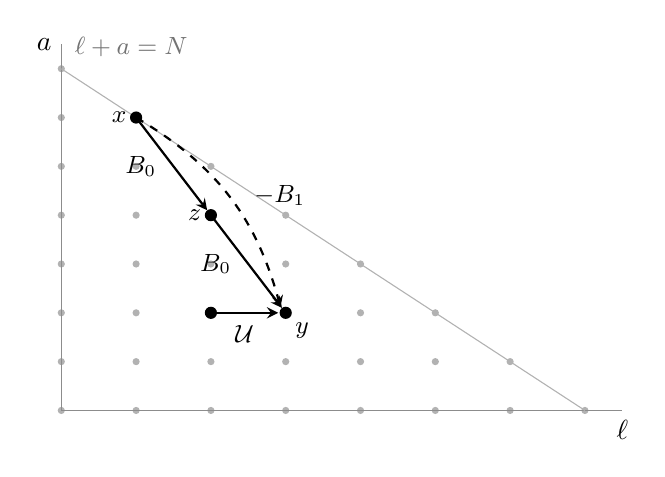
\begin{tikzpicture}[x=0.95cm,y=0.62cm,>=stealth]
\foreach \l in {0,...,7} \foreach \a in {0,...,7} {\pgfmathtruncatemacro{\s}{\l+\a}\ifnum\s<8 \fill[black!30] (\l,\a) circle (1.3pt);\fi}
\draw[black!45] (0,7.5) -- (0,0) -- (7.5,0);
\draw[black!30] (0,7) -- (7,0);
\node[anchor=north] at (7.5,0) {$\ell$};
\node[anchor=east] at (0,7.5) {$a$};
\node[black!55,anchor=south west,font=\small] at (0.05,7.05) {$\ell+a=N$};
\fill (1,6) circle (2.2pt) node[anchor=east,font=\small] {$x$\ };
\fill (2,4) circle (2.2pt) node[anchor=east,font=\small] {$z$\ };
\fill (3,2) circle (2.2pt) node[anchor=north west,font=\small] {$y$};
\fill (2,2) circle (2.2pt);
\draw[->,thick] (2,2) -- (2.9,2);
\node[anchor=north,font=\small] at (2.45,1.95) {$\mathcal U$};
\draw[->,thick] (1,6) -- (1.95,4.1);
\draw[->,thick] (2,4) -- (2.95,2.1);
\node[anchor=east,font=\small] at (1.4,5.0) {$B_0$};
\node[anchor=east,font=\small] at (2.4,3.0) {$B_0$};
\draw[->,thick,dashed] (1,6) to[bend left=22] (2.93,2.12);
\node[anchor=west,font=\small] at (2.45,4.4) {$-B_1$};
\end{tikzpicture}
\caption{The kernel recurrence of Lemma~\ref{lem:kernel-rec} on the triangle $\Omega$ ($N=7$). Every move raises $\ell$. The node $y=(\ell+1,a)$ receives the straight move $\mathcal U$ from $(\ell,a)$ and moves of index $j$ from nodes with smaller $\ell$; the moves of odd index carry a minus sign. The dashed move $-B_1$ from $x$, of displacement $(2,-4)$, is dominated by a quarter of the two-step paths from $x$ through $z=x+(1,-2)$ to $y$, made of two moves $B_0$ of even index (Lemma~\ref{lem:detours}); this gives $\mathcal P^2\geq4\mathcal Q$.}\label{fig:moves}
\end{figure}

\begin{table}[t]
\centering
\caption{The negative moves into $y=(\ell+1,a)$, for odd $j$, and the two-step paths through moves of even index that dominate them (Lemma~\ref{lem:detours}). The first step of a detour has index $0$, the second has index $j-1$.}\label{tab:detours}
\renewcommand{\arraystretch}{1.15}
\begin{tabular}{@{}lll@{}}
Negative move & Source node & Dominating detours\\\hline
$tA_j$ & $(\ell-j,\,a+2j+1)$ & $A_0$ then $B_{j-1}$; \ $B_0$ then $A_{j-1}$\\
$B_j$ & $(\ell-j,\,a+2j+2)$ & $B_0$ then $B_{j-1}$\\
$C_j$ & $(\ell-j-1,\,a+2j+2)$ & $B_0$ then $C_{j-1}$
\end{tabular}
\end{table}

\paragraph{A rescaled system and a kernel.}
Fix $r$ and put $t=(1-r)/\sqrt r\geq0$. If $p_i$ is defined by $p_0=1$ and $yp_i=a_ip_{i+1}+td_ip_i+d_ip_{i-1}$ $(0\leq i<N)$, then $R_i(x)=r^{i/2}p_i(x/\sqrt r)$, so the coefficients $H_{mn}^k$ in $p_mp_n=\sum_kH_{mn}^kp_k$ on the support satisfy $g(m,n;k)=r^{(m+n-k)/2}H_{mn}^k$. It suffices to show $H_{mn}^k\geq0$. Put
\[
e_i=\prod_{j=0}^{i-1}\frac{a_j}{d_{j+1}},\qquad E_i=e_ip_i.
\]
Then $yE_i=d_{i+1}E_{i+1}+td_iE_i+a_{i-1}E_{i-1}$ on the support for $0\leq i\leq N$, with the terms $d_{N+1}E_{N+1}$ and $a_{-1}E_{-1}$ omitted; at $i=N$ this is the terminal relation. Write $E_mE_n=\sum_kL_{mn}^kE_k$, so that $H_{mn}^k=L_{mn}^ke_k/(e_me_n)$, and
\[
K_k(z,w)=\sum_{m,n=0}^NL_{mn}^kz^mw^n.
\]
Let $\theta_z=z\,\partial_z$ and let $d(\theta)=\sum_k\nu_k\binom\theta k$ act on polynomials by $d(\theta_z)z^i=d_iz^i$. For $F(z)=\sum_{i=0}^NE_iz^i$ the recurrence reads $yF(z)=\mathcal L_zF(z)$ with
\[
\mathcal L_z=(z^{-1}+t-z)\,d(\theta_z)+z,
\]
because $d_0=0$ removes the term $z^{-1}E_0$ and $1-d_N=0$ removes the term $z^{N+1}E_N$. Applying this to $F(z)F(w)=\sum_kK_k(z,w)E_k$ in the two variables separately and comparing coefficients of the basis $E_k$ gives $(\mathcal L_z-\mathcal L_w)K_k=0$. Since $K_k$ is symmetric, $K_k=\sum_{\ell,a\geq0}\omega_{\ell,a}S^aZ^\ell$ with $S=z+w$, $Z=zw$, and $K_k(z,0)=z^k$ gives $\omega_{0,a}=\mathbf1_{a=k}$. As $K_k$ has degree at most $N$ in $z$, comparing the coefficients of $z^{\ell+a}w^\ell$ by induction on $\ell$ gives $\omega_{\ell,a}=0$ whenever $\ell+a>N$.

\paragraph{The kernel recurrence.}
Put $f_n(\ell)=\sum_{h\geq0}\binom\ell h\nu_{n+h}$ with $\nu_0=0$ and $\nu_k=0$ for $k>N$, so $f_0(\ell)=d_\ell$, and
\[
W_{p,q}(\ell,a)=\sum_{n\geq p}\binom{n-p+q}q\binom an f_n(\ell)\geq0,
\]
and $A_j=W_{2j+1,j}$, $B_j=W_{2j+2,j}$, $C_j=W_{2j+2,j+1}$.

\begin{lemma}\label{lem:kernel-rec}
For all $\ell,a\geq0$,
\begin{equation}\label{eq:kernel-rec}
\begin{aligned}
d_{\ell+1}\omega_{\ell+1,a}={}&a_{\ell+a}\,\omega_{\ell,a}+\sum_{j\geq0}(-1)^j\Big(t\,A_j(\ell-j,a+2j+1)\,\omega_{\ell-j,a+2j+1}\\
&+B_j(\ell-j,a+2j+2)\,\omega_{\ell-j,a+2j+2}\\
&+C_j(\ell-j-1,a+2j+2)\,\omega_{\ell-j-1,a+2j+2}\Big),
\end{aligned}
\end{equation}
where $a_i=1-d_i$ is extended by the polynomial $d_i$ for $i>N$ and terms with a negative index are omitted.
\end{lemma}
\begin{proof}
Since $S^aZ^\ell=\sum_i\binom ai z^{\ell+i}w^{\ell+a-i}$, Vandermonde's identity $\binom{\ell+i}k=\sum_{p+q=k}\binom\ell q\binom ip$ and $\binom ai\binom ip=\binom ap\binom{a-p}{i-p}$ give
\[
d(\theta_z)\,S^aZ^\ell=\sum_{p,q\geq0}\nu_{p+q}\binom\ell q\binom ap\,z^pS^{a-p}Z^\ell .
\]
Hence $(\mathcal L_z-\mathcal L_w)S^aZ^\ell$ equals $(z-w)S^aZ^\ell$ plus $\sum_{p,q}\nu_{p+q}\binom\ell q\binom ap S^{a-p}Z^\ell$ times $(z^{p-1}-w^{p-1})+t(z^p-w^p)-(z^{p+1}-w^{p+1})$. Divide by $z-w$, using $\chi_n=(z^{n+1}-w^{n+1})/(z-w)=\sum_{0\leq j\leq\lfloor n/2\rfloor}(-1)^j\binom{n-j}jS^{n-2j}Z^j$ for $n\geq0$, $\chi_{-1}=0$ and $(z^{-1}-w^{-1})/(z-w)=-Z^{-1}$. Since $\sum_q\binom\ell q\nu_{p+q}=f_p(\ell)$, the quotient is
\[
\begin{aligned}
&-d_\ell S^aZ^{\ell-1}+a_{\ell+a}S^aZ^\ell\\
&+\sum_{j\geq0}(-1)^j\Big(tA_j(\ell,a)S^{a-2j-1}Z^{\ell+j}+B_j(\ell,a)S^{a-2j-2}Z^{\ell+j}+C_j(\ell,a)S^{a-2j-2}Z^{\ell+j+1}\Big).
\end{aligned}
\]
Here $-d_\ell S^aZ^{\ell-1}$ comes from $p=0$; the term $a_{\ell+a}S^aZ^\ell$ combines $S^aZ^\ell$ with the parts $j=0$ of $-\chi_p$, which sum to $-d_{\ell+a}S^aZ^\ell$ by Vandermonde; and the three families from $\chi_{p-2}$, $t\chi_{p-1}$ and $-(\chi_p-S^p)$, whose coefficients $\binom{p-2-j}j$, $\binom{p-1-j}j$ and $\binom{p-1-j}{j+1}$ are those of $B_j$, $A_j$ and $C_j$. Summing over $\ell,a$ with weights $\omega_{\ell,a}$ and taking the coefficient of $S^aZ^\ell$ gives \eqref{eq:kernel-rec}, because the monomials $S^aZ^\ell$ are linearly independent.
\end{proof}

\paragraph{The log-concavity inequality.}
\begin{lemma}\label{lem:lc-ineq}
Let $(u_k)_{k\geq0}$ be nonnegative, finitely supported and log-concave without internal zeros, that is, its positive entries form an interval and $u_k^2\geq u_{k-1}u_{k+1}$ for all $k\geq1$, and put $f^u_n(\ell)=\sum_{h\geq0}\binom\ell hu_{n+h}$. Then $(u_k+u_{k+1})_{k\geq0}$ has the same property, hence so does $(f^u_n(\ell))_{n\geq0}$ for every $\ell\geq0$, and
\[
f^u_i(\ell)\,f^u_l(\ell+1)\geq f^u_0(\ell+1)\,f^u_{i+l}(\ell)\qquad(i,l\geq1,\ \ell\geq0).
\]
In particular, under the hypotheses of Theorem~\ref{thm:lc}, $f_i(\ell)\,f_l(\ell+1)\geq d_{\ell+1}\,f_{i+l}(\ell)$ for $i,l\geq1$ and $\ell\geq0$.
\end{lemma}
\begin{proof}
For a nonnegative finitely supported sequence $u$ that is log-concave without internal zeros, $v_i=u_i+u_{i+1}$ has the same property, since
$v_i^2-v_{i-1}v_{i+1}=(u_i^2-u_{i-1}u_{i+1})+(u_{i+1}^2-u_iu_{i+2})+(u_iu_{i+1}-u_{i-1}u_{i+2})$
and the last term is nonnegative by log-concavity. The sequence $(f^u_n(\ell))_n$ is obtained from $(u_n)_n$ by applying $u\mapsto v$ $\ell$ times. For such a sequence $g$, balanced products dominate: $g_ig_l\geq g_0g_{i+l}$ and $g_ig_{l+1}\geq g_1g_{i+l}$ for $i,l\geq1$. Adding these with $g=f^u(\ell)$ and using $g_l+g_{l+1}=f^u_l(\ell+1)$ and $g_0+g_1=f^u_0(\ell+1)$ gives the claim. Under the hypotheses of Theorem~\ref{thm:lc} the sequence $u=(0,\nu_1,\nu_2,\ldots)$ has the property, $f^u=f$, and $f_0(\ell+1)=d_{\ell+1}$.
\end{proof}

\begin{lemma}\label{lem:detours}
Under the hypotheses of Theorem~\ref{thm:lc}, for all $j\geq1$ and $\ell,a\geq0$,
\[
\begin{aligned}
A_0(\ell,a)B_{j-1}(\ell+1,a-1)+B_0(\ell,a)A_{j-1}(\ell+1,a-2)&\geq4d_{\ell+1}A_j(\ell,a),\\
B_0(\ell,a)B_{j-1}(\ell+1,a-2)&\geq4d_{\ell+1}B_j(\ell,a),\\
B_0(\ell,a)C_{j-1}(\ell+1,a-2)&\geq4d_{\ell+1}C_j(\ell,a),
\end{aligned}
\]
with $W_{p,q}(\ell,a)=0$ for $a<0$.
\end{lemma}
\begin{proof}
Use $A_0(\ell,a)\geq af_1(\ell)$ and $B_0(\ell,a)\geq\binom a2f_2(\ell)$, expand the second factor, apply Lemma~\ref{lem:lc-ineq} to $f_1(\ell)f_n(\ell+1)$ and $f_2(\ell)f_n(\ell+1)$, and use $a\binom{a-1}n=(n+1)\binom a{n+1}$ and $\binom a2\binom{a-2}n=\binom{n+2}2\binom a{n+2}$. After division by $d_{\ell+1}$ the three left sides are bounded below by $\sum_m\gamma_m\binom amf_m(\ell)$ with
\[
\gamma_m=\binom{m+1}2\binom{m-j-2}{j-1},\qquad\binom m2\binom{m-j-3}{j-1},\qquad\binom m2\binom{m-j-2}j,
\]
while the right sides are $4\sum_m\gamma'_m\binom amf_m(\ell)$ with $\gamma'_m=\binom{m-j-1}j$, $\binom{m-j-2}j$ and $\binom{m-j-1}{j+1}$. Where $\gamma'_m>0$ the quotients are
\[
\frac{jm(m+1)}{2(m-j-1)},\qquad\frac{jm(m-1)}{2(m-j-2)},\qquad\frac{(j+1)m(m-1)}{2(m-j-1)},
\]
on $m\geq2j+1$, $m\geq2j+2$ and $m\geq2j+2$ respectively. They increase with $j$ for fixed $m$; at $j=1$ their minima over integers are $5$, $5$ and $6$. All quotients exceed $4$, and $f_m(\ell)\geq0$.
\end{proof}

\begin{proof}[Proof of Theorem~\ref{thm:lc}]
Let $\Omega=\{(\ell,a):\ell,a\geq0,\ \ell+a\leq N\}$, on which $\omega$ is supported. Read \eqref{eq:kernel-rec} as moves into the node $(\ell+1,a)$, each divided by $d_{\ell+1}>0$: the straight move from $(\ell,a)$ with weight $a_{\ell+a}\geq0$ on $\Omega$, and for each $j$ the three moves from $(\ell-j,a+2j+1)$, $(\ell-j,a+2j+2)$, $(\ell-j-1,a+2j+2)$ with weights $tA_j$, $B_j$, $C_j$. Every move raises $\ell$. Let $\mathcal U$ be the straight moves, $\mathcal P$ the moves with $j$ even and $\mathcal Q$ the moves with $j$ odd, all with nonnegative weights, so that $\omega=\beta+(\mathcal U+\mathcal P-\mathcal Q)\omega$ with $\beta=\omega|_{\ell=0}$.

We claim $\mathcal P^2\geq4\mathcal Q$ entrywise. A move of $\mathcal Q$ with index $j$ from $x=(\ell,a)$ is matched by the two-step paths in $\mathcal P^2$ that start with $A_0$ or $B_0$ from $x$ (index $0$, landing at $(\ell+1,a-1)$ or $(\ell+1,a-2)$, which lie in $\Omega$) and continue with the move of the same type and index $j-1$ (even), as in Lemma~\ref{lem:detours}: $A_j$ by $A_0$ then $B_{j-1}$ and $B_0$ then $A_{j-1}$; $B_j$ by $B_0$ then $B_{j-1}$; $C_j$ by $B_0$ then $C_{j-1}$. These paths end at the target of the matched move, carry the same power of $t$, and have the extra denominator $d_{\ell+1}$ of the intermediate node. Distinct moves of $\mathcal Q$ have distinct displacements, so their paths are distinct, and Lemma~\ref{lem:detours} gives the claim.

Now show by induction on the level that $\omega\geq0$ and $\omega\geq\frac12\mathcal P\omega$. Both hold at $\ell=0$. If they hold below a node $y$ at level $\ell+1\geq1$, then, all weights being nonnegative, $(\mathcal P\omega)(y)\geq\frac12(\mathcal P^2\omega)(y)\geq2(\mathcal Q\omega)(y)$, and
\[
\omega(y)=(\mathcal U\omega)(y)+(\mathcal P\omega)(y)-(\mathcal Q\omega)(y)\geq\tfrac12(\mathcal P\omega)(y)\geq0.
\]
Hence all $\omega_{\ell,a}\geq0$, so $K_k$ has nonnegative coefficients in $z,w$, so $L_{mn}^k\geq0$, $H_{mn}^k\geq0$ and $g(m,n;k)\geq0$.
\end{proof}

\begin{remark}\label{rem:bernstein}
The argument is valid coefficientwise in $t$. With independent parameters in $yp_i=a_ip_{i+1}+ud_ip_i+vd_ip_{i-1}$, weighted homogeneity ($\deg y=\deg u=1$, $\deg v=2$) then shows that each linearization coefficient is a polynomial in $(u,v)$ with nonnegative coefficients: for $D=m+n-k\geq0$ it has the form $\sum_{0\leq j\leq\lfloor D/2\rfloor}h_ju^{D-2j}v^j$ with $h_j\geq0$, and it vanishes for $D<0$. Consequently every $g(m,n;k)$ of the array of Theorem~\ref{thm:lc}, as a function of $r$, equals $\sum_jh_jr^j(1-r)^{D-2j}$; multiplying the $j$-th term by $(r+(1-r))^j=1$ shows that its coefficients in the Bernstein basis of degree $D$ are $\binom Ds^{-1}\sum_{j\leq s\leq2j}h_j\binom j{s-j}\geq0$.
\end{remark}

Szwarc~\cite[\S5, Problem~2]{szwarc} records the positive range of the Krawtchouk polynomials as $0<p_0\leq1/2$.\footnote{In the author version of~\cite{szwarc}, \S5, Problem~2, printed p.~125, the displayed weights $\binom Nn p^{N-n}(1-p)^n$ have mean $N(1-p)$, whereas the displayed recurrence gives $K_1(x)=(x-pN)/((1-p)N)$, so that $\int K_1\,d\mu=(1-2p)/(1-p)$. The corollary fixes the convention directly: it uses the displayed weights and the normalization at the point carrying the weight $p^N$.}

\begin{corollary}[Full positive Krawtchouk range]\label{cor:kraw}
For every $N\geq1$ and $0<p_0\leq1/2$, Krawtchouk polynomials orthogonal for binomial weights $\binom Nj p_0^{N-j}(1-p_0)^j$ have nonnegative linearization when normalized at $j=0$.
\end{corollary}
\begin{proof}
To fix the convention without relying on a named recurrence, put $r=p_0/(1-p_0)\in(0,1]$, and let $Y_1,\ldots,Y_N$ be independent variables with values $1,-r$ of probabilities $p_0,1-p_0$. Their mean is zero and $Y_i^2=(1-r)Y_i+r$. The normalized elementary symmetric sums
\[
K_i(j)=\binom Ni^{-1}\sum_{|S|=i}\prod_{l\in S}Y_l
\]
depend only on the number $j$ of negative coordinates. They are orthogonal, because the expectation of two distinct squarefree monomials is zero: some independent mean-zero variable occurs once. Their weights in $j$ are exactly the stated binomial weights. With $x=N^{-1}\sum_lY_l=1-j/(N(1-p_0))$, multiplication by $x$ gives
\[
xK_i=\frac{N-i}{N}K_{i+1}+(1-r)\frac iN K_i+r\frac iN K_{i-1}.
\]
Indeed, in multiplying the elementary sum by $\sum_lY_l$, indices outside a subset give $(i+1)$ copies of each subset of size $i+1$; the linear part of $Y_l^2$ gives $(1-r)i$ copies of each subset of size $i$; and the constant part gives $r(N-i+1)$ copies of each subset of size $i-1$. Division by the binomial normalizers gives the displayed recurrence, including $i=N$. Its leading coefficient in $x$ is positive, its degree is $i$, and its value at $j=0$ is one. These properties identify the normalized orthogonal polynomials for the binomial measure. This is the array $K_{N,r}$; its profile $d_i=i/N$ has Newton coefficients $(1/N,0,\ldots,0)$, so Theorem~\ref{thm:lc} applies.
The range is sharp in this endpoint normalization: if $1/2<p_0<1$, then
$r=p_0/(1-p_0)>1$ and $g(1,1;1)=b_1=(1-r)/N<0$.
For $N=1$, this coefficient follows from the terminal relation.
\end{proof}

\begin{corollary}[Geometric arrays]\label{cor:additional}
For every $N\geq2$, $q>1$, and $0<r\leq1$, the array $G_{N,q,r}$ of \eqref{eq:parameters} has nonnegative linearization. In the normalization $R_0=1$, $R_1=x$, it is outside the Krawtchouk recurrence class.
\end{corollary}
\begin{proof}
Its increments are $d_i-d_{i-1}=q^{i-1}/[N]_q$, so its Newton coefficients $\nu_k=(q-1)^{k-1}/[N]_q$ are log-concave without internal zeros and Theorem~\ref{thm:lc} applies. For a Krawtchouk recurrence in this normalization the increments of $b_i+c_i$ are constant. Here their ratio is $q>1$ and $N\geq2$, so they are not constant. An affine change of the support transporting the same endpoint-normalized basis leaves the multiplication coefficients in the basis unchanged; it cannot remove this distinction.
\end{proof}

The arrays $G_{N,q,r}$ are the normalized recurrences of Koelink's construction~\cite[Theorems~3.1(ii) and~7.1]{koelink} with $r=1/p$; their polynomial interpretation is the dual $q$-Krawtchouk interpretation described after his Theorem~7.8. A proof of Corollary~\ref{cor:additional} by a finite algebra with positive multiplication, which needs only the geometric increments, is given in~\cite{P3}.

For some parameters both families come from distance-regular graphs. Dividing the intersection array of such a graph by its valency gives an array satisfying \eqref{eq:basic}, and its linearization coefficients are positive multiples of the intersection numbers $p^k_{mn}$, hence nonnegative~\cite{bcn,vdkt}. For an integer $s\geq2$, the Hamming graph $H(N,s)$ gives $K_{N,r}$ with $r=1/(s-1)$; a dual polar graph of diameter $N$ with classical parameters $(N,q,0,q^e)$ gives $G_{N,q,r}$ with $r=q^{-e}$. Corollaries~\ref{cor:kraw} and~\ref{cor:additional} cover the full parameter ranges.

\section{Szwarc's quadratic system}\label{sec:szwarc}

Problem~2 of~\cite[\S5]{szwarc} does not stop at the Krawtchouk recurrence. With his parameter written as $p_0$, Szwarc introduces the symmetric recurrence of length $2N+1$
\begin{equation}\label{eq:szwarc-q}
yQ_{2n}=(N-n)Q_{2n+1}+nQ_{2n-1},\qquad
yQ_{2n-1}=(1-p_0)Q_{2n}+p_0Q_{2n-2},
\end{equation}
records that $Q_{2n}(y)$ is the Krawtchouk polynomial $K_n(y^2)$ of his recurrence, states that the $Q_n$ have nonnegative linearization for $p_0\leq1/2$, and asks for a general criterion that would handle this case. His Theorem~3.3 for infinite symmetric systems does not apply. In the normalization \eqref{eq:szwarc-q} its monotonicity hypotheses hold, and its hypothesis $\alpha_n\leq\gamma_n$ holds at odd indices exactly when $p_0\leq1/2$; at an even index $2n$ it reads $n\leq N-n$ and fails in the upper half. Some failure of this kind is forced in every finite system, whose terminal upward coefficient vanishes. We derive the positivity of \eqref{eq:szwarc-q} from Theorem~\ref{thm:lc} through a quadratic decomposition of symmetric finite systems.

Put $M=2N$, $R_{2n}(t)=Q_{2n}(\sqrt Nt)$ and $R_{2n-1}(t)=\sqrt N\,Q_{2n-1}(\sqrt Nt)$. Substitution in \eqref{eq:szwarc-q} shows that the $R_k$ satisfy \eqref{eq:recurrence}, with $N$ replaced by $M$, for the array
\begin{equation}\label{eq:qarray}
b_k=0,\qquad
(a_{2n},c_{2n})=\Big(\frac{N-n}{N},\frac nN\Big),\qquad
(a_{2n-1},c_{2n-1})=(1-p_0,\,p_0).
\end{equation}
It satisfies \eqref{eq:basic} with $M$ in place of $N$ whenever $0<p_0<1$. The two normalizations differ by positive factors and a positive dilation, so they have the same product coefficients up to positive factors.

Szwarc uses the quadratic transformation~\cite[\S3.5]{szwarc} to pass from a symmetric system to its even part. In~\cite{szwarc1992} a parity-split monotonicity criterion for symmetric infinite systems gives property (P) of the generalized Chebyshev polynomials and, through their even parts, Gasper's result for the Jacobi polynomials with $\alpha\geq\beta$ and $\alpha+\beta+1\geq0$; in~\cite{szwarc1996} the same route gives property (P) of Askey--Wilson polynomials for a range of parameters. In both, positivity passes from a symmetric system to its even part. For the finite systems of classical association schemes, bipartite halves and antipodal quotients give quadratic transformations of the polynomials, which Chihara and Stanton~\cite{chiharastanton} derive from a quadratic transformation of the Askey--Wilson polynomials. The decomposition of a symmetric system into its even and odd components, and the identities relating their products, are standard, and we claim no priority for them. What we use is the converse implication for finite systems: positivity of a symmetric system, including the products beyond the terminal degree, follows from positivity of its two components, both read off from its coefficients, which need not come from a scheme. Any criterion for nonsymmetric finite systems therefore becomes a criterion for symmetric ones. For a family of infinite systems a result of this kind is known: Kahler~\cite{kahler} solved Problem~1 of~\cite[\S5]{szwarc} by showing that the generalized Chebyshev polynomials, the quadratic transforms of the Jacobi polynomials, have property (P) exactly for the parameters for which the Jacobi polynomials $R_n^{(\alpha,\beta)}$ have it. His result concerns that family; Theorem~\ref{thm:decomp} below is a reduction for arbitrary finite symmetric systems.

\begin{theorem}[Quadratic decomposition]\label{thm:decomp}
Let $N\geq2$, and let $a_k,c_k$ $(0\leq k\leq2N)$ with $b\equiv0$ satisfy \eqref{eq:basic} with $2N$ in place of $N$. Put $a_k=c_k=0$ for $k\notin[0,2N]$, and define the even component
\[
\hat a_n=a_{2n}a_{2n+1},\quad \hat b_n=c_{2n}a_{2n-1}+a_{2n}c_{2n+1},\quad \hat c_n=c_{2n}c_{2n-1}\qquad(0\leq n\leq N)
\]
and the odd component
\[
\check a_n=a_{2n+1}a_{2n+2},\quad \check b_n=a_{2n+1}c_{2n+2}+c_{2n+1}a_{2n},\quad \check c_n=c_{2n+1}c_{2n}\qquad(0\leq n<N).
\]
After the affine normalization $(\hat a_n,\hat b_n,\hat c_n)\mapsto(\hat a_n,\hat b_n-\hat b_0,\hat c_n)/\hat a_0$, and likewise for the odd component, these arrays satisfy \eqref{eq:basic} on the indices $0,\ldots,N$ and $0,\ldots,N-1$. If both have nonnegative linearization, so does the symmetric array. More precisely, with $\hat g$ and $\check g$ the product coefficients of the components and terms with indices out of range omitted,
\[
g(2a,2b;2c)=\hat g(a,b;c),\qquad
g(2a,2b+1;2c+1)=a_{2a}\,\check g(a,b;c)+c_{2a}\,\check g(a-1,b;c),
\]
the coefficients with $m+n+k$ odd vanish, and $g(2a+1,2b+1;2c)\int R_{2c}^2\,d\mu=g(2c,2a+1;2b+1)\int R_{2b+1}^2\,d\mu$. Conversely, nonnegative linearization of the symmetric array implies that of its even component.
\end{theorem}
\begin{proof}
Since $b\equiv0$, the matrix $J$ is conjugate to $-J$ by $\operatorname{diag}((-1)^i)$, which fixes $e_0$; hence the measure of Lemma~\ref{lem:finite} is symmetric and $R_k(-t)=(-1)^kR_k(t)$. By symmetry $R_{2n}(t)=P_n(t^2)$ and $R_{2n+1}(t)=tL_n(t^2)$ for polynomials $P_n$, $L_n$ of degree $n$. Applying \eqref{eq:recurrence} twice gives, with $x=t^2$,
\[
xP_n=\hat a_nP_{n+1}+\hat b_nP_n+\hat c_nP_{n-1},\qquad
xL_n=\check a_nL_{n+1}+\check b_nL_n+\check c_nL_{n-1}.
\]
The row sums of the components equal $a_{2n}+c_{2n}=1$ and $a_{2n+1}+c_{2n+1}=1$; the coefficients $\hat a_n,\check a_n$ are positive below the last index and vanish there, and $\hat c_n,\check c_n>0$ for $n\geq1$. Hence the normalized arrays, which describe the same polynomials in the variable $(x-\hat b_0)/\hat a_0$ (respectively $(x-\check b_0)/\check a_0$), satisfy \eqref{eq:basic}. The terminal relation $tR_{2N}=c_{2N}R_{2N-1}$ on the support $\Sigma$ of the symmetric system, applied once and twice, gives the terminal relations of $P$ on $\{t^2:t\in\Sigma\}$ and of $L$ on $\{t^2:t\in\Sigma,\ t\neq0\}$. These sets have $N+1$ and $N$ points, because $\Sigma$ is symmetric with $2N+1$ points and contains $0$. By Lemma~\ref{lem:finite} they are the supports of the two components.

The identity $tR_{2n}=a_{2n}R_{2n+1}+c_{2n}R_{2n-1}$ gives $P_n=a_{2n}L_n+c_{2n}L_{n-1}$ on the support of $L$; for $n=N$ it is the terminal relation, with $a_{2N}=0$. Hence, on $\Sigma\setminus\{0\}$,
\[
R_{2a}R_{2b+1}=t\big(a_{2a}L_aL_b+c_{2a}L_{a-1}L_b\big)=\sum_c\big(a_{2a}\check g(a,b;c)+c_{2a}\check g(a-1,b;c)\big)R_{2c+1},
\]
and both sides vanish at $t=0$. Similarly $R_{2a}R_{2b}=(P_aP_b)(t^2)=\sum_c\hat g(a,b;c)R_{2c}$ on $\Sigma$. Uniqueness of expansions on $\Sigma$ gives the displayed formulas. The vanishing for $m+n+k$ odd and the relation for two odd indices follow from the symmetry of the measure and from $g(m,n;k)\int R_k^2\,d\mu=\int R_mR_nR_k\,d\mu$. The converse holds because $\hat g(a,b;c)=g(2a,2b;2c)$.
\end{proof}

Combined with Theorem~\ref{thm:lc}, the decomposition gives a parity-split criterion of the same shape as Szwarc's Theorem~3.3: separate conditions on the even-indexed and the odd-indexed coefficients.

\begin{corollary}[Parity-split criterion]\label{cor:parity}
Let $N\geq1$ and let a symmetric array $(b\equiv0)$ on the indices $0,\ldots,2N$ satisfy \eqref{eq:basic}. Suppose that
\begin{enumerate}
\item the odd downward coefficients are constant, $c_{2n+1}=p_0$, with $0<p_0\leq1/2$;
\item the even downward coefficients $d_n=c_{2n}$ have positive increments $d_n-d_{n-1}$, $1\leq n\leq N$, forming a geometric progression with ratio $q\geq1$.
\end{enumerate}
Then the array has nonnegative linearization. With $r=p_0/(1-p_0)$ and $N\geq2$, its normalized even and odd components are \eqref{eq:parameters} with parameters $(N,q,r)$ and $(N-1,q,r/q)$, respectively. For $N=1$ the odd component consists only of $L_0=1$ and the array is \eqref{eq:qarray}. If $1/2<p_0<1$ in (i) and (ii) holds, then $g(2,2;2)<0$.
\end{corollary}
\begin{proof}
For $N=1$ the array is $a_0=1$, $c_1=p_0$, $a_1=1-p_0$, $c_2=1$, with support $\{-1,0,1\}$ and $R_1=t$, $R_2=(t^2-p_0)/(1-p_0)$. On the support $R_1^2=(1-p_0)R_2+p_0$, $R_1R_2=R_1$ and $R_2^2=\frac{p_0}{1-p_0}+\frac{1-2p_0}{1-p_0}R_2$, as evaluation at $t=0,\pm1$ shows; all coefficients are nonnegative for $p_0\leq1/2$, and $g(2,2;2)<0$ for $p_0>1/2$. Let $N\geq2$. The even component has $\hat a_n=(1-d_n)(1-p_0)$, $\hat b_n=d_n(1-p_0)+(1-d_n)p_0$ and $\hat c_n=d_np_0$, so $\hat a_0=1-p_0$, $\hat b_0=p_0$, and its normalization is $(1-d_n,\,(1-r)d_n,\,rd_n)$. Its profile $d_n$ has geometric increments, so its Newton coefficients are proportional to $(q-1)^{k-1}$ and log-concave without internal zeros, and $0<r\leq1$. For the odd component, $\check a_n=(1-p_0)(1-d_{n+1})$, $\check b_n=(1-p_0)d_{n+1}+p_0(1-d_n)$ and $\check c_n=p_0d_n$. Geometric increments give $d_{n+1}-d_1=qd_n$, so the normalization is
\[
\Big(\frac{1-d_{n+1}}{1-d_1},\ \frac{(q-r)d_n}{1-d_1},\ \frac{rd_n}{1-d_1}\Big).
\]
Its profile $qd_n/(1-d_1)$ has geometric increments with ratio $q$, and its downward coefficients are $r/q\leq1$ times the profile. Theorem~\ref{thm:lc} applies to both components, and Theorem~\ref{thm:decomp} concludes. Comparison with \eqref{eq:parameters}, using $d_n=[n]_q/[N]_q$ and $1-d_1=q[N-1]_q/[N]_q$, identifies the parameters. For $p_0>1/2$, $g(2,2;2)=\hat g(1,1;1)$ is the normalized diagonal coefficient $(1-r)d_1<0$ (for $N=1$ see above).
\end{proof}

\begin{theorem}[Szwarc's quadratic system]\label{thm:szwarc}
Let $N\geq1$ and $0<p_0\leq1/2$. The array \eqref{eq:qarray} has a symmetric positive orthogonality measure on $2N+1$ points, and for all $0\leq m,n\leq 2N$
\[
R_mR_n=\sum_{k=0}^{2N}g(m,n;k)R_k,\qquad g(m,n;k)\geq0,\qquad\sum_k g(m,n;k)=1
\]
on that support. If $1/2<p_0<1$, then $g(2,2;2)<0$.
\end{theorem}
\begin{proof}
Lemma~\ref{lem:finite} gives a positive measure on $2N+1$ points, and it is symmetric because $b\equiv0$ (proof of Theorem~\ref{thm:decomp}). The array \eqref{eq:qarray} satisfies the hypotheses of Corollary~\ref{cor:parity} with $c_{2n+1}=p_0$ and $d_n=n/N$, that is, with $q=1$, which gives nonnegative linearization for $p_0\leq1/2$ and $g(2,2;2)<0$ for $1/2<p_0<1$. The coefficients sum to one because $R_k(1)=1$ and $1$ lies in the support, since $J\boldsymbol1=\boldsymbol1$.
\end{proof}

The even component of \eqref{eq:qarray} is the Krawtchouk array $K_{N,r}$ with $r=p_0/(1-p_0)$, so that $Q_{2n}(y)$ is a Krawtchouk polynomial in $y^2$, as Szwarc notes, and its odd component is $K_{N-1,r}$. A second proof of Theorem~\ref{thm:szwarc}, by a graded version of the algebra of~\cite{P3}, and explicit coefficient neighborhoods of \eqref{eq:qarray} are given there.

\section{Ratios given by weights}\label{sec:vary}

We use the notation of Section~\ref{sec:lc}, extended as follows. The Newton coefficients of a sequence $(u_i)_{0\leq i\leq N}$ are $\Delta^ku(0)=\sum_{i\leq k}(-1)^{k-i}\binom kiu_i$, so that $u_n=\sum_k\binom nk\Delta^ku(0)$. For a nonnegative, finitely supported sequence $(u_k)_{k\geq0}$ that is log-concave without internal zeros in the sense of Lemma~\ref{lem:lc-ineq} we form $f_n(\ell)=f^u_n(\ell)$ and
\[
W_{p,q}(\ell,a)=\sum_{n\geq p}\binom{n-p+q}q\binom anf_n(\ell)
\]
as in Section~\ref{sec:lc}, and say from which sequence they are formed; without qualification, $A_j=W_{2j+1,j}$, $B_j=W_{2j+2,j}$ and $C_j=W_{2j+2,j+1}$ are formed from the Newton coefficients of the profile, as there. For $i\geq1$ with $d_i>0$ we write $\rho(i)=c_i/d_i$ for the ratio. Section~\ref{sec:lc} proves property (P) for constant ratios by expanding the product coefficients in a kernel $\omega_{\ell,a}$ on $\Omega=\{(\ell,a):\ell,a\geq0,\ \ell+a\leq N\}$, which satisfies a recurrence in $\ell$ whose moves have weights formed from the $W_{p,q}$, and by matching each move of odd index with two-step detours through moves of even index (Lemmas~\ref{lem:kernel-rec} and~\ref{lem:detours}). We extend that argument.

The kernel argument also works directly for normalized arrays, with independent diagonal and downward coefficients. Let $a_i+b_i+c_i=1$ for $0\leq i\leq N$, with $b_0=c_0=0$, $a_N=0$, $a_i>0$ for $i<N$ and $c_i>0$ for $i\geq1$. Write
\[
\kappa_k=\sum_{i=0}^k(-1)^{k-i}\binom kic_i,\qquad\beta_k=\sum_{i=0}^k(-1)^{k-i}\binom kib_i\qquad(1\leq k\leq N),
\]
with $\kappa_k=\beta_k=0$ for $k=0$ and $k>N$, and put $\varphi_n(\ell)=\sum_{h\geq0}\binom\ell h\kappa_{n+h}$ and $\psi_n(\ell)=\sum_{h\geq0}\binom\ell h\beta_{n+h}$, so that $\varphi_0(\ell)=c_\ell$ and $\psi_0(\ell)=b_\ell$ for $\ell\leq N$.

\begin{theorem}[Varying ratio]\label{thm:lc-vary}
Let $(\kappa_k)$ be log-concave without internal zeros and $\beta_k\geq0$ for all $k$. Suppose that for $0\leq\ell\leq N-1$
\[
\psi_1(\ell)\,\varphi_n(\ell+1)\geq c_{\ell+1}\,\psi_{n+1}(\ell)\quad(n\geq2),\qquad\varphi_2(\ell)\,\psi_n(\ell+1)\geq c_{\ell+1}\,\psi_{n+2}(\ell)\quad(n\geq1).
\]
Then the system has nonnegative linearization.
\end{theorem}

\begin{corollary}\label{cor:lc-vary}
If $(\kappa_k)$ is log-concave without internal zeros and $\beta_k=w_k\kappa_k$ for $k\geq1$ with $w_1\geq w_2\geq\cdots\geq0$, then the system has nonnegative linearization. The ratio $c_i/(b_i+c_i)$ is nondecreasing in $i\geq1$, and it is constant when $w$ is constant on the support of $\kappa$; these are the arrays of Theorem~\ref{thm:lc}.
\end{corollary}

For example, if $c$ is a convex quadratic in $i$ ($\kappa_1,\kappa_2>0$, $\kappa_k=0$ for $k\geq3$) and $b_i=w_1\kappa_1i+w_2\kappa_2\binom i2$ with $w_1>w_2\geq0$, scaled so that $b_N+c_N=1$, the ratio $c_i/(b_i+c_i)$ increases strictly. The hypotheses exclude the counterexample recorded in Appendix~\ref{app:frontier}, whose diagonal coefficients $b=(0,1,1,1)/91$ have Newton coefficients of both signs. For $N\geq2$, a strictly increasing linear ratio on a linear profile violates the corollary's assumptions because $\Delta^2b(0)<0$; Proposition~\ref{prop:lc-quad} covers it when $b$ is nondecreasing.

\begin{proof}[Proof of Theorem~\ref{thm:lc-vary}]
Put $e_i=\prod_{j<i}a_j/c_{j+1}$ and $E_i=e_iR_i$. Then $xE_i=c_{i+1}E_{i+1}+b_iE_i+a_{i-1}E_{i-1}$ on the support. The out-of-range terms are omitted: at the endpoints, $xE_0=c_1E_1$ and $xE_N=b_NE_N+a_{N-1}E_{N-1}$. The series $F=\sum_iE_iz^i$ satisfies $xF=\mathcal L_zF$ with
\[
\mathcal L_z=z^{-1}c(\theta_z)+b(\theta_z)+z\bigl(1-b(\theta_z)-c(\theta_z)\bigr),
\]
where $c(\theta)=\sum_k\kappa_k\binom\theta k$ and $b(\theta)=\sum_k\beta_k\binom\theta k$. As in Section~\ref{sec:lc}, $K_k=\sum_{m,n}L_{mn}^kz^mw^n$, with $E_mE_n=\sum_kL_{mn}^kE_k$, satisfies $(\mathcal L_z-\mathcal L_w)K_k=0$, and $K_k=\sum\omega_{\ell,a}S^aZ^\ell$ with $\omega_{0,a}=\mathbf1_{a=k}$ and $\omega_{\ell,a}=0$ for $\ell+a>N$. The computation in the proof of Lemma~\ref{lem:kernel-rec} gives
\[
\frac{(\mathcal L_z-\mathcal L_w)S^aZ^\ell}{z-w}=S^aZ^\ell+\sum_{p\geq0}\binom apS^{a-p}Z^\ell\Bigl(\varphi_p(\ell)(\chi_{p-2}-\chi_p)+\psi_p(\ell)(\chi_{p-1}-\chi_p)\Bigr),
\]
with $\chi_{-2}=-Z^{-1}$ and $\chi_{-1}=0$. Collecting terms as there, with $W_{p,q}$ formed from $\varphi$ and $W^\psi_{p,q}$ from $\psi$, gives
\[
\begin{aligned}
c_{\ell+1}\omega_{\ell+1,a}={}&a_{\ell+a}\,\omega_{\ell,a}+\sum_{j\geq0}(-1)^j\Big(A^\psi_j(\ell-j,a+2j+1)\,\omega_{\ell-j,a+2j+1}\\
&+B_j(\ell-j,a+2j+2)\,\omega_{\ell-j,a+2j+2}\\
&+\bigl(C_j+C^\psi_j\bigr)(\ell-j-1,a+2j+2)\,\omega_{\ell-j-1,a+2j+2}\Big),
\end{aligned}
\]
where $A^\psi_j=W^\psi_{2j+1,j}$, $C^\psi_j=W^\psi_{2j+2,j+1}$, and $B_j=W_{2j+2,j}$, $C_j=W_{2j+2,j+1}$. The straight weight is $1-c_{\ell+a}-b_{\ell+a}=a_{\ell+a}$, extended polynomially beyond $N$, and $\beta_0=0$. Up to this point no hypothesis of the theorem has been used: the recurrence holds for every normalized array, whatever the signs of its diagonal coefficients. Under the hypotheses, all weights are nonnegative on $\Omega$.

For $j\geq1$, $0\leq\ell\leq N-1$ and $a\geq0$, the following detour inequalities hold, with weights having a negative second argument interpreted as zero:
\[
\begin{aligned}
A^\psi_0(\ell,a)B_{j-1}(\ell+1,a-1)+B_0(\ell,a)A^\psi_{j-1}(\ell+1,a-2)&\geq4c_{\ell+1}A^\psi_j(\ell,a),\\
B_0(\ell,a)B_{j-1}(\ell+1,a-2)&\geq4c_{\ell+1}B_j(\ell,a),\\
B_0(\ell,a)\bigl(C_{j-1}+C^\psi_{j-1}\bigr)(\ell+1,a-2)&\geq4c_{\ell+1}\bigl(C_j+C^\psi_j\bigr)(\ell,a).
\end{aligned}
\]
The proof of Lemma~\ref{lem:detours} applies, with the lower bounds $A^\psi_0(\ell,a)\geq a\psi_1(\ell)$ and $B_0(\ell,a)\geq\binom a2\varphi_2(\ell)$. Lemma~\ref{lem:lc-ineq} for $\varphi$ handles the products $\varphi_2(\ell)\varphi_n(\ell+1)$. The two hypotheses of the theorem handle $\psi_1(\ell)\varphi_n(\ell+1)$ for $n\geq2$ and $\varphi_2(\ell)\psi_n(\ell+1)$ for $n\geq1$, which are the indices that occur. The moves $C_j$ and $C^\psi_j$ have the same displacement and are treated as one move. With this, the proof of Theorem~\ref{thm:lc} gives $\omega\geq0$, hence $L_{mn}^k\geq0$ and $g(m,n;k)=L_{mn}^ke_k/(e_me_n)\geq0$.
\end{proof}

\begin{proof}[Proof of Corollary~\ref{cor:lc-vary}]
Set $w_0=w_1$; since $\kappa_0=0$, this leaves $\beta_0=0$. Fix $\ell$ and write $G_i=\varphi_i(\ell)$, $H_i=\psi_i(\ell)$ and $u_x=\binom\ell{x-i}$. For $i\geq0$,
\[
H_iG_{i+1}-H_{i+1}G_i=\sum_{x,y\geq i}u_xu_y\kappa_x\kappa_{y+1}(w_x-w_{y+1}).
\]
Terms with $x\leq y$ are nonnegative, and terms with $x=y+1$ vanish. The map $(x,y)\mapsto(y+1,x-1)$ is a bijection from the terms with $x\geq y+2$ onto those with $i+1\leq x\leq y$; the remaining terms have $x=i$. A term and its image sum to $\kappa_x\kappa_{y+1}(w_{y+1}-w_x)(u_{y+1}u_{x-1}-u_xu_y)\geq0$, because $w$ is nonincreasing and the zero-extended binomial coefficients are log-concave. Hence $H_{i+1}G_i\leq H_iG_{i+1}$.

Since the support of $(G_i)$ is an interval and $\beta_k=0$ where $\kappa_k=0$, chaining gives $H_{n+1}G_1\leq H_1G_{n+1}$, $H_{n+2}G_n\leq H_nG_{n+2}$ and $H_{n+2}G_{n+1}\leq H_{n+1}G_{n+2}$. Lemma~\ref{lem:lc-ineq} with $(i,l)=(1,n)$ and $(2,n)$ reads $G_1(G_n+G_{n+1})\geq CG_{n+1}$ and $G_2(G_n+G_{n+1})\geq CG_{n+2}$, where $C=G_0+G_1=c_{\ell+1}$ and $G_n+G_{n+1}=\varphi_n(\ell+1)$. Since $G_1\geq\kappa_1>0$, $H_1(G_n+G_{n+1})\geq C H_1G_{n+1}/G_1\geq CH_{n+1}$. If $G_{n+2}>0$, then $G_2(H_n+H_{n+1})\geq G_2H_{n+2}(G_n+G_{n+1})/G_{n+2}\geq CH_{n+2}$; if $G_{n+2}=0$, then $H_{n+2}=0$. These are the two hypotheses of Theorem~\ref{thm:lc-vary}. The case $i=0$ of the first display, with $\beta_0=\kappa_0=0$, reads $b_{\ell+1}c_\ell\leq b_\ell c_{\ell+1}$; for $1\leq\ell<N$, division by $c_\ell c_{\ell+1}>0$ shows that $b_i/c_i$ is nonincreasing and $c_i/(b_i+c_i)$ is nondecreasing. If $w$ is constant on the support of $\kappa$, then $b$ is proportional to $c$, and with $d=b+c$ the array is that of Theorem~\ref{thm:lc}.
\end{proof}

For arrays that are quadratic in the index, concave diagonal coefficients are allowed.

\begin{proposition}[Quadratic arrays]\label{prop:lc-quad}
Let $b_n=\beta_1n+\beta_2\binom n2$ and $c_n=\kappa_1n+\kappa_2\binom n2$ $(0\leq n\leq N)$ define an array as above. If $\kappa_2\geq0$, $\kappa_2+\beta_2\geq0$ and $b_0\leq b_1\leq\cdots\leq b_N$, then the system has nonnegative linearization.
\end{proposition}

\begin{proof}
In the recurrence of the proof of Theorem~\ref{thm:lc-vary}, which holds for every array, $\varphi_n=\psi_n=0$ for $n\geq3$. So all moves with $j\geq1$ vanish, and the moves with $j=0$ have the weights $A^\psi_0(\ell,a)=\sum_{n\geq1}\binom an\psi_n(\ell)=b_{\ell+a}-b_\ell$, $B_0(\ell,a)=\binom a2\kappa_2$ and $(C_0+C^\psi_0)(\ell,a)=\binom a2(\kappa_2+\beta_2)$. These and the straight weights $a_{\ell+a}$ are nonnegative on $\Omega$, so $\omega\geq0$ by induction on $\ell$, and $g(m,n;k)\geq0$ as in the proof of Theorem~\ref{thm:lc-vary}.
\end{proof}

With the linear profile $d_n=n/N$ and the ratio $c_n/d_n=r+\kappa n/N$ ($1\leq n\leq N$, $r>0$, $\kappa\geq0$), one has $\kappa_2=2\kappa/N^2$ and $\kappa_2+\beta_2=0$ for $N\geq2$. For $N=1$, property (P) follows directly from $R_1^2=c_1R_0+b_1R_1$ when $b_1\geq0$. So every linearly increasing ratio with a linear profile and nondecreasing $b$ has property (P); $b$ is nondecreasing exactly when $\kappa\leq(1-r)N/(2N-1)$. Exact computations~\cite{code} show that each of the three hypotheses is needed: dropping any one of them gives quadratic arrays with a negative coefficient at $N\leq3$.

\section{Linearly and quadratically increasing ratios}\label{sec:affine}
For curved profiles, linearly increasing ratios need not satisfy the hypotheses of Theorem~\ref{thm:lc-vary}: the Newton coefficients of $b$ of order at least $3$ can be negative, and then some moves of even index in the recurrence of its proof have negative weight and no two-step detour. A resummation of the positive moves handles this.

\begin{theorem}[Linearly increasing ratio]\label{thm:lc-affine}
Let $0=d_0<d_1<\cdots<d_N=1$ have Newton coefficients that are log-concave without internal zeros, let $0<r\leq1$ and $\kappa\geq0$, and put $\rho_i=r+\kappa i/N$, $a_i=1-d_i$, $b_i=(1-\rho_i)d_i$ and $c_i=\rho_id_i$. If $b$ is nondecreasing, then the system has nonnegative linearization. The condition that $b$ be nondecreasing is equivalent to $\kappa\bigl(N+d_{N-1}/(1-d_{N-1})\bigr)\leq N(1-r)$.
\end{theorem}

For the linear profile $d_i=i/N$ the condition reads $\kappa\leq\frac N{2N-1}(1-r)$, and these are arrays of Proposition~\ref{prop:lc-quad}. For a convex profile $d_{N-1}\leq(N-1)/N$, so the admitted range of $\kappa$ contains $[0,\frac N{2N-1}(1-r)]$. When $r<1$, this containment is strict for a nonlinear profile. For example, $N=4$, $d_i=(2^i-1)/15$, $r=1/2$ and $\kappa=2/5$ are admitted, with $b=(0,2/75,3/50,7/75,1/10)$, although $(2N-1)\kappa/N=7/10>1-r$.

\begin{proof}
Write $s=1-r$ and $t=\kappa/N$, and let $f_n(\ell)=\Delta^nd(\ell)$ and $\nu_i=\Delta^id(0)$ be as in Section~\ref{sec:lc}, with $\nu_{-1}=\nu_0=0$. For $0\leq i<N$ put $R_i=d_i/f_1(i)$; then $f_1(i)\geq\nu_1>0$, and log-concavity of $(f_n(i))_{n\geq0}$ gives $R_{i+1}-R_i=\bigl(f_1(i)^2-d_if_2(i)\bigr)/\bigl(f_1(i)f_1(i+1)\bigr)\geq0$. Since $b_{i+1}-b_i=f_1(i)\bigl(s-t(i+1)-tR_i\bigr)$ and the bracket is nonincreasing in $i$, $b$ is nondecreasing exactly when its last increment is nonnegative, that is, when $t(N+R_{N-1})\leq s$ with $R_{N-1}=d_{N-1}/(1-d_{N-1})$; this is the stated condition. In particular $tN\leq s$. Since $c_i=(r+ti)d_i$ and $b_i=(s-ti)d_i$, the Leibniz rule for differences gives, for $\ell\geq0$ and $1\leq n\leq N-\ell$, which includes every index occurring in the moves on $\Omega$,
\[
\varphi_n(\ell)=(r+t(\ell+n))f_n(\ell)+tnf_{n-1}(\ell),\qquad\psi_n(\ell)=h_n(\ell)-v_n(\ell),
\]
with $h_n(\ell)=(s-t(\ell+n))f_n(\ell)$ and $v_n(\ell)=tnf_{n-1}(\ell)$; both are nonnegative when $\ell+n\leq N$. (Outside this range the formulas need not hold, because the Newton coefficients of $b$ and $c$ are set to zero beyond $N$.) Extend $\nu$ by zero outside $1\leq i\leq N$ and put $\widehat\kappa_i=p_i\nu_i+q_i\nu_{i-1}$ $(i\geq1)$, $\widehat\kappa_0=0$, with $p_i=r+ti$ and $q_i=ti$; the Newton sequence $\kappa$ of $c$ is the truncation of $\widehat\kappa$ at $N$. Then
\[
\begin{aligned}
\widehat\kappa_i^2-\widehat\kappa_{i-1}\widehat\kappa_{i+1}={}&p_i^2(\nu_i^2-\nu_{i-1}\nu_{i+1})+q_i^2(\nu_{i-1}^2-\nu_{i-2}\nu_i)\\
&+q_{i-1}p_{i+1}(\nu_i\nu_{i-1}-\nu_{i-2}\nu_{i+1})+t^2(\nu_{i-1}\nu_{i+1}+\nu_{i-2}\nu_i+2\nu_i\nu_{i-1}),
\end{aligned}
\]
and each term is nonnegative by log-concavity of $\nu$. The positive support of $\widehat\kappa$ is that of $\nu$ when $t=0$ and extends it by one index when $t>0$, an interval in both cases. Truncation at $N$ preserves log-concavity and interval support, so $\kappa$ is log-concave without internal zeros, and Lemma~\ref{lem:lc-ineq} applies to $f$ and to $\varphi$.

\emph{Moves.} We use the recurrence of the proof of Theorem~\ref{thm:lc-vary}, which holds for every array. For $j\geq1$ split $A^\psi_j=H_j-V_j$, where $H_j=W^h_{2j+1,j}$ and $V_j=W^v_{2j+1,j}$ are formed from $h_n$ and $v_n$ in place of $\psi_n$; both are nonnegative on $\Omega$. Keep $A^\psi_0(\ell,a)=b_{\ell+a}-b_\ell$ as one move; it is nonnegative because $b$ is nondecreasing. The weights $B_j$, formed from $\varphi$, and $C_j+C^\psi_j=W^f_{2j+2,j+1}$, formed from $f$, are nonnegative. Write $C'_j=C_j+C^\psi_j$.

\emph{Detours.} All detour inequalities below are asserted for source nodes $(\ell,a)\in\Omega$; in the mixed products the occurring indices satisfy $n\leq a-2$, hence $\ell+n+2\leq N$. Since $\varphi_2(\ell)\geq(r+t(\ell+1))f_2(\ell)$ and $c_{\ell+1}=(r+t(\ell+1))d_{\ell+1}$, Lemma~\ref{lem:lc-ineq} for $f$ gives
\[
\begin{gathered}
\varphi_2(\ell)f_n(\ell+1)\geq c_{\ell+1}f_{n+2}(\ell),\qquad\varphi_2(\ell)h_n(\ell+1)\geq c_{\ell+1}h_{n+2}(\ell),\\
\varphi_2(\ell)v_n(\ell+1)\geq\tfrac{n}{n+2}\,c_{\ell+1}v_{n+2}(\ell)\quad(n\geq2),
\end{gathered}
\]
using $s-t(\ell+n+1)\geq s-t(\ell+n+2)\geq0$ for the second and Lemma~\ref{lem:lc-ineq} with indices $(2,n-1)$ for the third. As in the proof of Lemma~\ref{lem:detours}, with $B_0(\ell,a)\geq\binom a2\varphi_2(\ell)$, for $0\leq\ell\leq N-1$ and second factors at $(\ell+1,a-2)$,
\[
\begin{gathered}
B_0B_{j-1}\geq4c_{\ell+1}B_j\ (j\geq1),\qquad B_0H_{j-1}\geq6c_{\ell+1}H_j\ (j\geq2),\\
B_0V_{j-1}\geq6c_{\ell+1}V_j\ (j\geq2),\qquad B_0C'_{j-1}\geq6c_{\ell+1}C'_j\ (j\geq1).
\end{gathered}
\]
The first uses Lemma~\ref{lem:lc-ineq} for $\varphi$. The coefficient ratios are, on $m\geq2j+2$, $2j+1$, $2j+1$ and $2j+2$ respectively,
\[
\frac{jm(m-1)}{2(m-j-2)},\qquad\frac{jm(m-1)}{2(m-j-1)},\qquad\frac{j(m-1)(m-2)}{2(m-j-1)},\qquad\frac{(j+1)m(m-1)}{2(m-j-1)};
\]
they increase with $j$ and are at least $5$, $10$, $6$ and $6$. Finally,
\begin{equation}\label{eq:affine-key}
A^\psi_0(\ell,a)B_0(\ell+1,a-1)+B_0(\ell,a)A^\psi_0(\ell+1,a-2)\geq c_{\ell+1}\bigl(4H_1(\ell,a)-2V_1(\ell,a)\bigr).
\end{equation}
Only $a\geq3$ needs proof. Put $u_n=f_n(\ell)$, $y_n=\binom anu_n$, $D=u_0+u_1=d_{\ell+1}$, $\alpha=s-t(\ell+a)$,
\[
\begin{gathered}
X=\sum_{n\geq1}y_n,\qquad Y=\sum_{n\geq2}y_n,\qquad J=\sum_{n=2}^{a-1}\tbinom{a-1}nu_n,\\
X'=\sum_{j\geq1}\tbinom{a-2}j(u_j+u_{j+1}),\qquad Y'=\sum_{j\geq2}\tbinom{a-1}j(u_j+u_{j+1}),
\end{gathered}
\]
so that $X=au_1+Y$, $X'=(a-2)u_1+J$ and $Y'=Y-(a-1)u_2$. Then $A^\psi_0(\ell,a)=\alpha X-tau_0$ and $A^\psi_0(\ell+1,a-2)=(\alpha+t)X'-t(a-2)D$; both are nonnegative, and the two weights $B_0$ are at least $(r+t(\ell+1))Y'$ and $(r+t(\ell+1))Y$. With $H_*=\sum_{n\geq3}(n-2)y_n$ and $T=\sum_{n\geq2}(n-3)(a-n)y_n$ one has $H_1=\sum_{n\geq3}(n-2)(\alpha+t(a-n))y_n$ and, after a shift of index, $V_1=t\sum_{n\geq2}(n-1)(a-n)y_n$, so $4H_1-2V_1=4\alpha H_*+2tT$. Since $c_{\ell+1}=(r+t(\ell+1))D$, it suffices to show
\begin{equation}\label{eq:affine-red}
(\alpha X-tau_0)Y'+Y\bigl((\alpha+t)X'-t(a-2)D\bigr)\geq D(4\alpha H_*+2tT).
\end{equation}
The coefficient of $\alpha$ in the difference of the two sides is $K=XY'+YX'-4DH_*$. By Lemma~\ref{lem:lc-ineq}, $u_i(u_j+u_{j+1})\geq Du_{i+j}$ for $i,j\geq1$, so $XY'\geq au_1Y'\geq D\sum_{n\geq3}ny_n$ and $YX'\geq\binom a2u_2X'\geq D\sum_{n\geq3}\binom n2y_n$; hence $K\geq\frac D2\sum_{n\geq3}\bigl((n-3)(n-4)+4\bigr)y_n\geq0$, and \eqref{eq:affine-red} holds when $t=0$. Let $t>0$. Monotonicity of $b$ at $\ell+a-1$ gives $\alpha\geq tR_{\ell+a-1}\geq tR_\ell=tu_0/u_1$, so it suffices to prove \eqref{eq:affine-red} at $\alpha=tu_0/u_1$. Both sides are homogeneous of degree two in $(u_n)$; take $u_1=1$ and write $z=u_0$ and $q=u_2$. If $q=0$, then $u_n=0$ for $n\geq2$ and both sides vanish. Otherwise $0\leq z\leq1/q$ by log-concavity. At $\alpha=tz$ the two weights $A^\psi_0$ are $tzY$ and $t(z+1)J$, and \eqref{eq:affine-red} divided by $t$ reads $F(z)\geq0$, where
\[
\begin{aligned}
F(z)&=zYY'+(z+1)YJ-(z+1)(4zH_*+2T)\\
&=(1-qz)F(0)+qzF(1/q)+4H_*z(1/q-z),
\end{aligned}
\]
the second form holding because $F$ is quadratic with leading coefficient $-4H_*$. It remains to show $F(0)\geq0$ and $F(1/q)\geq0$. Put $L_3=\frac32$, $L_n=\frac{n(n+2)}6$ for $n\geq4$, and $E_n=\frac{2(n^2-5)}{n+1}$. In $YJ$ keep, for each $n$, the product with indices $(2,2)$ if $n=3$, and the products with indices $(2,n-1)$ and $(3,n-2)$ if $n\geq4$; by log-concavity with $u_1=1$, $u_iu_{n+1-i}\geq u_n$, and $\binom{a-1}j\geq\binom{a-i}j$, so $YJ\geq\sum_{n=3}^{a-1}L_n(a-n)y_n$. In $Y$ keep the term $\binom a2q$; as $q(u_{n-1}+u_n)\geq(q+1)u_n$ for $n\geq3$, $YY'\geq(q+1)\sum_{n=3}^a\frac{n(a-1)}2y_n$. Since $L_n\geq2(n-3)$,
\[
F(0)=YJ-2T\geq2(a-2)y_2+\sum_{n=3}^{a-1}\bigl(L_n-2(n-3)\bigr)(a-n)y_n\geq0.
\]
Using $u_n\leq qu_{n-1}$ and a shift of index, $\frac4qH_*+2T\leq\sum_{n=2}^{a-1}E_n(a-n)y_n$, where $E_2<0$. As $L_n+\frac n2\geq E_n$ for $n\geq3$,
\[
\frac{F(1/q)}{1+1/q}=YJ+\frac{YY'}{q+1}-\frac4qH_*-2T\geq\sum_{n=3}^{a-1}\Bigl(L_n+\frac n2-E_n\Bigr)(a-n)y_n\geq0.
\]
The numerical facts used are $L_3=\frac32\geq0$, $L_3+\frac32=3\geq E_3=2$, and, for $n\geq4$, $6(L_n-2(n-3))=(n-5)^2+11$ and $6(n+1)(L_n+\frac n2-E_n)=n^3-6n^2+5n+60>0$.

\emph{Resummation.} Regard the moves as operators on functions on $\Omega$, each divided by $c$ at the destination level; all strictly raise $\ell$, and inequalities between operators are entrywise. Let $P$ and $Q$ be the sums of the $B_j$ with $j$ even and odd, $C=C_+-C_-$ with $C_\pm$ the sums of the $C'_j$ with $j$ even and odd, $H_+$ and $H_-$ the sums of the $H_j$ with $j\geq2$ even and $j\geq3$ odd, $V_+$ and $V_-$ the sums of the $V_j$ with $j$ odd and $j\geq2$ even, $A_0$ the operator of $A^\psi_0$, and $U$ the straight moves. The recurrence reads $\omega=\beta+(U+P-Q+C+A)\omega$ with $A=A_0+H_+-H_--H_1+V_+-V_-$ and $\beta=\omega|_{\ell=0}\geq0$. The inequalities above give
\[
P^2\geq4Q,\quad H_+P\geq6H_-,\quad V_+P\geq6V_-,\quad C_+P\geq6C_-,\quad A_0P+PA_0+2V_1\geq4H_1.
\]
Let $G=(I-P/2)^{-1}=\sum_{m=0}^N(P/2)^m\geq0$. Then $PG=GP=2(G-I)$ and $(I-P/6)G=\frac23G+\frac13I$, so $G(H_+-H_-)G\geq GH_+(I-P/6)G\geq0$, $GCG\geq0$ and $G(V_+-V_-)G\geq\frac23GV_1G$. Hence
\[
\begin{aligned}
GAG&\geq G\bigl(A_0-H_1+\tfrac23V_1\bigr)G\geq G\bigl(A_0-\tfrac14(A_0P+PA_0)+\tfrac16V_1\bigr)G\\
&=\tfrac12(GA_0+A_0G)+\tfrac16GV_1G\geq0.
\end{aligned}
\]
With $R=U+P^2/4-Q\geq0$, the operator $M=G(R+C+A)G$ is nonnegative and strictly raises $\ell$. Since $(I-P/2)^2\omega=\beta+(R+C+A)\omega$, the function $v=(I-P/2)\omega$ satisfies $v=G\beta+Mv$. Therefore $\omega=G\sum_{q=0}^NM^qG\beta\geq0$, and $g(m,n;k)\geq0$ as in the proof of Theorem~\ref{thm:lc-vary}.
\end{proof}

\begin{theorem}[Convex quadratic ratio]\label{thm:lc-quadratic}
Let $0=d_0<d_1<\cdots<d_N=1$ have Newton coefficients that are log-concave without internal zeros, let $\rho(x)=r+tx+\tau\binom x2$ with $r>0$ and $t,\tau\geq0$, and put $a_i=1-d_i$, $b_i=(1-\rho(i))d_i$ and $c_i=\rho(i)d_i$. If $b$ is nondecreasing, then the system has nonnegative linearization.
\end{theorem}

This contains Theorem~\ref{thm:lc-affine} ($\tau=0$). As in the proof of that theorem, $b_{i+1}-b_i=f_1(i)\bigl(1-\rho(i+1)-(t+\tau i)R_i\bigr)$ with a nonincreasing bracket, so $b$ is nondecreasing exactly when $t(N+R)+\tau\bigl(\binom N2+(N-1)R\bigr)\leq1-r$ with $R=d_{N-1}/(1-d_{N-1})$. The Newton coefficients of $c$ need not be log-concave: for $d_i=i/4$ and $\rho(x)=\frac12+\binom x2/40$ they are $(1/8,1/80,3/160,0)$. The proof below replaces their log-concavity by a weighted detour inequality.

\begin{proof}
Write $f_n(\ell)=\Delta^nd(\ell)$, $\Delta\rho(x)=t+\tau x$ and $R_i=d_i/f_1(i)$, which is nondecreasing as in the proof of Theorem~\ref{thm:lc-affine}. Since $b_{i+1}-b_i=f_1(i)\bigl(1-\rho(i+1)-\Delta\rho(i)R_i\bigr)$ and $b$ is nondecreasing, $1-\rho(m+1)\geq\Delta\rho(m)R_m$ for $0\leq m<N$, and $\rho(i)\leq1$ for $i\leq N$. For $\ell+n\leq N$ the Leibniz rule gives, all at $\ell$,
\[
\varphi_n=\rho(\ell+n)f_n+n\Delta\rho(\ell+n-1)f_{n-1}+\binom n2\tau f_{n-2},\qquad\psi_n=h_n-v_n-w_n,
\]
with $h_n=(1-\rho(\ell+n))f_n$, $v_n=n\Delta\rho(\ell+n-1)f_{n-1}$ and $w_n=\binom n2\tau f_{n-2}$; here $\varphi_n$, $h_n$, $v_n$ and $w_n$ are nonnegative, while $\psi_n$ need not be.

\emph{Moves.} In the recurrence of the proof of Theorem~\ref{thm:lc-vary}, keep $A^\psi_0=b_{\ell+a}-b_\ell\geq0$ and split $A^\psi_j=H_j-V_j-W_j$ for $j\geq1$, where $H_j$, $V_j$ and $W_j$ are $W_{2j+1,j}$ formed from $h_n$, $v_n$ and $w_n$; the weights $B_j$, formed from $\varphi$, and $C'_j=C_j+C^\psi_j=W^f_{2j+2,j+1}$ are nonnegative. With the signs $(-1)^j$, the moves $W_j$ behave like the $V_j$.

\emph{Detours of $H$, $V$, $W$ and $C'$.} All detours are asserted for sources $(\ell,a)\in\Omega$, with second factors at $(\ell+1,a-2)$, marked by a prime. Since $\varphi_2(\ell)\geq\rho(\ell+1)f_2(\ell)$ and $c_{\ell+1}=\rho(\ell+1)d_{\ell+1}$, Lemma~\ref{lem:lc-ineq} for $f$ gives, for $n\leq a-2$,
\[
\begin{gathered}
\varphi_2f_n'\geq c_{\ell+1}f_{n+2},\qquad\varphi_2h_n'\geq c_{\ell+1}h_{n+2},\\
(n+1)(n+2)\varphi_2v_n'\geq n^2c_{\ell+1}v_{n+2},\qquad(n+1)(n+2)\varphi_2w_n'\geq n(n-1)c_{\ell+1}w_{n+2},
\end{gathered}
\]
the last two for $n\geq3$. The second uses $1-\rho(\ell+n+1)\geq1-\rho(\ell+n+2)\geq0$; the third uses Lemma~\ref{lem:lc-ineq} with indices $(2,n-1)$ and $(n+1)\Delta\rho(\ell+n)-n\Delta\rho(\ell+n+1)=t+\tau\ell\geq0$; the fourth uses indices $(2,n-2)$. As in the proof of Lemma~\ref{lem:detours}, with $B_0(\ell,a)\geq\binom a2\varphi_2(\ell)$ and $\binom a2\binom{a-2}{m-2}=\binom am\binom m2$,
\[
\begin{gathered}
B_0H_{j-1}'\geq10c_{\ell+1}H_j,\qquad B_0V_{j-1}'\geq\tfrac92c_{\ell+1}V_j,\qquad B_0W_{j-1}'\geq3c_{\ell+1}W_j\quad(j\geq2),\\
B_0\,C'_{j-1}(\ell+1,a-2)\geq6c_{\ell+1}C'_j\quad(j\geq1).
\end{gathered}
\]
The coefficient ratios are $\frac{jm(m-1)}{2(m-j-1)}$, $\frac{j(m-2)^2}{2(m-j-1)}$ and $\frac{j(m-2)(m-3)}{2(m-j-1)}$ on $m\geq2j+1$, and $\frac{(j+1)m(m-1)}{2(m-j-1)}$ on $m\geq2j+2$; they increase with $j$, and at the smallest $j$ the bounds are $(m-5)(m-6)\geq0$, $(m-5)(2m-7)\geq0$, $m\geq5$ and $(m-3)(m-4)\geq0$.

\emph{Detour of $B$.} We show, for $n\geq2$ and $\ell+n+2\leq N$,
\begin{equation}\label{eq:quad-B}
(n+1)(n+2)\,\varphi_2(\ell)\varphi_n(\ell+1)\geq8(n-1)\,c_{\ell+1}\varphi_{n+2}(\ell).
\end{equation}
Granting this, $B_0(\ell,a)\geq\binom a2\varphi_2(\ell)$, \eqref{eq:quad-B} with $n=m-2$, $\binom a2\binom{a-2}{m-2}=\binom am\binom m2$ and $\binom m2\frac{8(m-3)}{m(m-1)}=4(m-3)$ give
\[
\begin{aligned}
B_0(\ell,a)B_{j-1}(\ell+1,a-2)&\geq4c_{\ell+1}\sum_{m\geq2j+2}(m-3)\binom{m-j-3}{j-1}\binom am\varphi_m(\ell)\\
&\geq4c_{\ell+1}B_j(\ell,a)
\end{aligned}
\]
for $j\geq1$, because $(m-3)\binom{m-j-3}{j-1}-\binom{m-j-2}j=\binom{m-j-3}{j-1}\frac{(j-1)(m-2)}j\geq0$. (With constant $1$ in place of $\frac{(n+1)(n+2)}{8(n-1)}$, \eqref{eq:quad-B} can fail: for $N=20$, $d_i=(2^i-1)/(2^{20}-1)$, $r=\frac12$, $t=0$, $\tau=10^{-3}$ one gets $\varphi_2(16)\varphi_2(17)<c_{17}\varphi_4(16)$.)

To prove \eqref{eq:quad-B}, put $u_k=f_k(\ell)$, so that $f_k(\ell+1)=u_k+u_{k+1}$, and $p=\rho(\ell+1)$, $K_n=(n+1)(n+2)$, $L_n=8(n-1)$. Both sides are homogeneous of degree two in $u$; take $u_1=1$ and write $z=u_0$, $q=u_2$. By convexity and log-concavity, $0\leq z\leq\ell$ and $zq\leq1$. If $q=0$ or $u_n=0$, then $\varphi_{n+2}(\ell)=0$. Otherwise put $y=u_{n+1}/u_n\in[0,q]$. Log-concavity gives $u_{n+2}\leq y^2u_n$, and for $n\geq3$ also $u_{n-1}\geq u_n/q$ and $u_{n-2}\geq u_n/q^2$. Hence $\varphi_n(\ell+1)\geq u_n\mathcal L(y)$ and $\varphi_{n+2}(\ell)\leq u_n\mathcal T(y)$, where
\[
\mathcal T(y)=\rho(\ell+n+2)y^2+(n+2)\Delta\rho(\ell+n+1)y+\binom{n+2}2\tau,
\]
$\mathcal L(y)=\rho(\ell+n+1)(1+y)+n\Delta\rho(\ell+n)(1+q^{-1})+\binom n2\tau(q^{-1}+q^{-2})$ for $n\geq3$, and $\mathcal L(y)=\rho(\ell+3)(1+y)+2\Delta\rho(\ell+2)(1+q^{-1})+\tau(z+1)q^{-1}$ for $n=2$ (exact). In both cases $\mathcal L(y)=A+By$ with $A\geq B\geq0$, so $\mathcal L(0)\geq\mathcal L(q)/(1+q)$; and $\mathcal T(q)\geq(1+q)\mathcal T(0)$ because $(n+2)\Delta\rho(\ell+n+1)\geq(n+2)(n+1)\tau$. The function $\mathcal F(y)=K_n\varphi_2(\ell)\mathcal L(y)-L_np(z+1)\mathcal T(y)$ is concave with $\mathcal F(0)\geq\mathcal F(q)/(1+q)$, so it suffices that $\mathcal F(q)\geq0$, which is \eqref{eq:quad-B} for the configuration $u_0=z$, $u_k=q^{k-1}$ $(k\geq1)$.

Next we reduce to $z=\min(\ell,1/q)$. For $n\geq3$, only $\varphi_2(\ell)=A_2+\tau z$ and $c_{\ell+1}=p(z+1)$ depend on $z$, where $A_2=\rho(\ell+2)q+2\Delta\rho(\ell+1)\geq\tau$, so $\varphi_2(\ell)/(z+1)$ is nonincreasing in $z$. For $n=2$, write also $\varphi_2(\ell+1)=G_2+\tau(z+1)$ with $G_2=\rho(\ell+3)q(1+q)+2\Delta\rho(\ell+2)(1+q)$. For $z\leq Z\leq\ell$ the quotient $\varphi_2(\ell)\varphi_2(\ell+1)/(z+1)$ at $z$ minus its value at $Z$ equals $(Z-z)\bigl(G_2(A_2-\tau)/((z+1)(Z+1))-\tau^2\bigr)\geq0$, since $G_2(A_2-\tau)\geq2(\ell+2)(2\ell+1)\tau^2\geq(\ell+1)^2\tau^2$.

For the remaining configurations we use the following polynomial inequality. For an integer $n\geq2$ and reals $h\geq1$, $p,\tau\geq0$ and $s\geq(h-1)\tau$, put $A=p+(2h-1)s+h^2\tau$, $B=p+nh(s+\tau)+\binom n2h^2\tau$ and $C=p+((n+2)h-1)s+\binom{n+2}2h^2\tau$. Then
\begin{equation}\label{eq:quad-cert}
K_nAB-L_npC\geq0.
\end{equation}
Indeed, $K_nAB-L_npC$ is nondecreasing in $s$ (its $ps$-coefficient is $a_n((n+2)h-1)$ with $a_n=n^2-5n+10>0$, and its other $s$-dependent coefficients are nonnegative), and at $s=(h-1)\tau$ it equals $a_np^2+C_n(h)p\tau+D_n(h)\tau^2$, where $C_n(h)=\frac12\bigl(h^2U_n+h(10n^2+14n-60)+2a_n\bigr)$, $U_n=n^4-4n^3-21n^2+12n+60$ and $D_n(h)=\frac12h^2n(n+1)^2(n+2)(3h^2-3h+1)$. For $n\geq7$ all three coefficients are nonnegative, since $U_n=k^4+24k^3+189k^2+502k+144$ with $k=n-7$. For $2\leq n\leq6$, $4a_nD_n-C_n^2$ is a polynomial in $v=h-1$ with positive coefficients:
\[
\begin{array}{c|ccccc}
n&v^0&v^1&v^2&v^3&v^4\\\hline
2&576&2880&5616&4992&1664\\
3&1520&6240&9744&7200&2160\\
4&6300&27000&42660&30600&8604\\
5&25200&126000&229500&184800&56000\\
6&62720&376320&774144&677376&216576
\end{array}
\]
so $a_np^2+C_np\tau+D_n\tau^2=a_n\bigl(p+\frac{C_n\tau}{2a_n}\bigr)^2+\frac{4a_nD_n-C_n^2}{4a_n}\tau^2\geq0$.

If $1/q\leq\ell$, take $z=1/q$, $h=1+1/q$ and $s=t+\tau\ell\geq(h-1)\tau$. For the configuration above, $\mathcal F(q)$ divided by $q(1+q)$ equals $K_nAB-L_npC$, which is nonnegative by \eqref{eq:quad-cert}.

If $\ell<1/q$, take $z=\ell$, and write $w=1/q-\ell>0$, $h_0=\ell+1$, $h=h_0+w$ and $s=t+\tau\ell$. With $A(w)=p+(2h-1)s+\tau\bigl((\ell+2)h-\ell-1\bigr)$ and $B(w)$, $C(w)$ as above (with this $h$), $\mathcal F(q)$ divided by $q^2$ equals $\mathcal E_n(w)=K_n(h_0+w)A(w)B(w)-L_nh_0pC(w)$ for $n\geq3$, and $\mathcal E_2(w)-12A(w)\tau w(\ell+w)^2$ for $n=2$. At $w=0$ both equal $h_0(K_nAB-L_npC)$ with $h=h_0$, which is nonnegative by \eqref{eq:quad-cert}. Expanding in $w$, with $\bar A=A(0)-p$ and $\bar B=B(0)-p$, every coefficient of $w$, $w^2$, $w^3$ and $w^4$ is a sum of nonnegative terms: for $n\geq3$,
\[
\begin{aligned}
[w]&=K_np^2+p(a_1t+b_1\tau)+K_n\bigl(\bar A\bar B+h_0(\eta\bar B+\bar A\theta)\bigr),\\
[w^2]&=p(a_2t+b_2\tau)+K_n\bigl(\eta\bar B+\bar A\theta+h_0(\eta\theta+\bar A\epsilon)\bigr),\\
[w^3]&=K_n\bigl(\eta\theta+A(0)\epsilon+h_0\eta\epsilon\bigr),\qquad[w^4]=K_n\eta\epsilon,
\end{aligned}
\]
where
\[
\begin{gathered}
\eta=2s+(\ell+2)\tau,\qquad\theta=n(s+\tau)+n(n-1)\tau h_0,\qquad\epsilon=\tbinom n2\tau,\\
a_1=(n+2)\bigl(2\ell(n^2-n+6)+2n^2-3n+11\bigr),\qquad a_2=K_n(n+2),\\
b_1=\tfrac{n+2}2(\ell^2P_n+\ell Q_n+R_n),\qquad b_2=\tfrac{K_n}2\bigl(3n(n-3)(\ell+1)+14\ell+12\bigr),
\end{gathered}
\]
with $P_n=3k^3+15k^2+6k+8$, $Q_n=6k^3+30k^2+20k+16$ and $R_n=3k^3+15k^2+16k+16$ for $k=n-3$; for $n=2$ the coefficients of $w$, $w^2$ and $w^3$ are
\[
\begin{aligned}
&12p^2+4(16\ell+13)pt+8(\ell+1)(2\ell+3)p\tau+48(\ell+1)(3\ell+2)t^2\\&\qquad+12(36\ell^3+92\ell^2+76\ell+21)t\tau+12(27\ell^4+93\ell^3+114\ell^2+62\ell+13)\tau^2,\\
&48pt+12(2\ell+3)p\tau+24(6\ell+5)t^2\\&\qquad+12(36\ell^2+67\ell+29)t\tau+12(27\ell^3+78\ell^2+67\ell+19)\tau^2,\\
&12\bigl(2s+(\ell+2)\tau\bigr)\bigl(2t+(3\ell+5)\tau\bigr).
\end{aligned}
\]
This proves \eqref{eq:quad-B}.

\emph{Key inequality.} We show, for $(\ell,a)\in\Omega$ with $a\geq3$,
\begin{equation}\label{eq:quad-key}
A^\psi_0(\ell,a)B_0(\ell+1,a-1)+B_0(\ell,a)A^\psi_0(\ell+1,a-2)\geq c_{\ell+1}\bigl(4H_1-2V_1-W_1\bigr)(\ell,a).
\end{equation}
Use the notation of the proof of Theorem~\ref{thm:lc-affine} ($u_n=f_n(\ell)$, $y_n$, $D$, $X$, $Y$, $X'$, $Y'$, $J$, $H_*$, $T$), and put $\alpha=1-\rho(\ell+a)$, $s=\Delta\rho(\ell+a-1)$, $p=\rho(\ell+1)$ and $Z=\sum_{n\geq2}\binom{a-n}2y_n$. Then $\alpha\geq sR_{\ell+a-1}\geq su_0/u_1$ and $s\geq\tau(a-1)$. Backward differences give
\[
\begin{aligned}
A^\psi_0(\ell,a)&=\alpha X-sau_0+\tau\tbinom a2u_0,\\
A^\psi_0(\ell+1,a-2)&=(\alpha+s)X'-s(a-2)D+\tau\tbinom{a-1}2D,
\end{aligned}
\]
both nonnegative, and $B_0(\ell,a)\geq pY$, $B_0(\ell+1,a-1)\geq pY'$, $c_{\ell+1}=pD$. Since $1-\rho(\ell+n)=\alpha+(a-n)s-\tau\binom{a-n}2$, reindexing gives $4H_1-2V_1=4\alpha H_*+2sT+4\tau Z$ and $W_1=\tau\sum_{n\geq1}n\binom{a-n}2y_n$. The argument of the proof of Theorem~\ref{thm:lc-affine} with $s$ in place of $t$, keeping the surplus of the two endpoints ($F(0)\geq2(a-2)y_2$ and $F(1/q)\geq\frac23(1+1/q)(a-2)y_2$, from the term $n=2$ and $E_2=-\frac23$), shows
\[
(\alpha X-sau_0)Y'+Y\bigl((\alpha+s)X'-s(a-2)D\bigr)-D(4\alpha H_*+2sT)\geq\tfrac23sD(a-2)y_2
\]
for $\alpha u_1\geq su_0$; the right side of this bound is linear in $z=u_0/u_1$ and is subtracted before the interpolation. With $s\geq\tau(a-1)$, the difference of the two sides of \eqref{eq:quad-key} divided by $p$ is therefore at least
\[
\begin{aligned}
\tau\Bigl(\tbinom a2u_0Y'+D\Bigl[&\tbinom{a-1}2y_1+\tfrac{(a-2)(a+11)}6y_2+(2a-5)y_3\\
&+\sum_{n\geq4}\Bigl(\tbinom{a-1}2+(n-4)\tbinom{a-n}2\Bigr)y_n\Bigr]\Bigr)\geq0.
\end{aligned}
\]

\emph{Resummation.} With $W_\pm$ the sums of the $W_j$ with $j$ odd and $j\geq2$ even, the recurrence reads as in the proof of Theorem~\ref{thm:lc-affine} with $A=A_0-H_1+(H_+-H_-)+(V_+-V_-)+(W_+-W_-)$, and the inequalities above give $P^2\geq4Q$, $H_+P\geq10H_-$, $V_+P\geq\frac92V_-$, $W_+P\geq3W_-$, $C_+P\geq6C_-$ and $A_0P+PA_0+2V_1+W_1\geq4H_1$. Since $(I-P/\mu)G=(1-\frac2\mu)G+\frac2\mu I$, one has $G(H_+-H_-)G\geq0$, $GCG\geq0$, $G(V_+-V_-)G\geq\frac59GV_1G$ and $G(W_+-W_-)G\geq\frac13GW_1G$, hence
\[
\begin{aligned}
GAG&\geq G\bigl(A_0-\tfrac14(A_0P+PA_0)+\tfrac1{18}V_1+\tfrac1{12}W_1\bigr)G\\
&=\tfrac12(GA_0+A_0G)+\tfrac1{18}GV_1G+\tfrac1{12}GW_1G\geq0.
\end{aligned}
\]
With $U+P^2/4-Q\geq0$ this gives $M\geq0$, and (P) follows as before.
\end{proof}

\section{Ratios of higher degree}\label{sec:higher}
For profiles of Newton degree at most two the ratio can have any degree, provided the Newton coefficients of $c$ are nonnegative and log-concave without internal zeros; no key inequality is needed.

\begin{theorem}[Low-degree profiles]\label{thm:lc-lowdeg}
Let $d_i=\nu_1i+\nu_2\binom i2$ with $\nu_1>0$, $\nu_2\geq0$ and $d_N=1$, let $c_0=0$, and suppose that the Newton coefficients $\kappa_k=\Delta^kc(0)$, $1\leq k\leq N$, are log-concave without internal zeros. Put $a_i=1-d_i$ and $b_i=d_i-c_i$. If $b$ is nondecreasing, then the system has nonnegative linearization.
\end{theorem}

\begin{proof}
We use the recurrence of the proof of Theorem~\ref{thm:lc-vary}, which holds for every array, with $\varphi_n(\ell)=\Delta^nc(\ell)$, $\psi_n(\ell)=\Delta^nb(\ell)$ and $f_n(\ell)=\Delta^nd(\ell)$ for the polynomial extensions. Since $f_n=0$ for $n\geq3$, every move $A^\psi_j$ with $j\geq1$, which involves only $n\geq2j+1\geq3$, equals $-\widetilde B_j$ with $\widetilde B_j=W_{2j+1,j}$ formed from $\varphi$; the moves $C_j+C^\psi_j=W^f_{2j+2,j+1}$ vanish for $j\geq1$, and $C_0+C^\psi_0=\binom a2\nu_2\geq0$. The weight $A^\psi_0(\ell,a)=b_{\ell+a}-b_\ell$ is nonnegative on $\Omega$, as are the straight weights and all $B_j$ and $\widetilde B_j$, since $(\varphi_n(\ell))_n$ is obtained from $(\kappa_k)$ by the shifts of Lemma~\ref{lem:lc-ineq} and is therefore nonnegative and log-concave without internal zeros. Lemma~\ref{lem:lc-ineq} for $\varphi$ gives, as in Lemma~\ref{lem:detours}, $B_0(\ell,a)B_{j-1}(\ell+1,a-2)\geq4c_{\ell+1}B_j(\ell,a)$ for $j\geq1$, and with $B_0(\ell,a)\geq\binom a2\varphi_2(\ell)$ also $B_0(\ell,a)\widetilde B_{j-1}(\ell+1,a-2)\geq4c_{\ell+1}\widetilde B_j(\ell,a)$ for $j\geq2$, because the coefficient quotients $jm(m-1)/(2(m-j-1))$ on $m\geq2j+1$ are at least $10$. In the resummation of the proof of Theorem~\ref{thm:lc-affine} take $H=0$ and $V_j=\widetilde B_j$; the key inequality is then trivial, and $M\geq0$ gives (P).
\end{proof}

\begin{corollary}\label{cor:lc-lowdeg}
In Theorem~\ref{thm:lc-lowdeg} let $c_i=\rho(i)d_i$ with $\rho(x)=\sum_k\rho_k\binom xk$, where $(\rho_k)_{k\geq0}$ is nonnegative and log-concave without internal zeros and $\rho_0>0$. Then the Newton coefficients of $c$ are log-concave without internal zeros. Hence every such ratio, of any degree, with nondecreasing $b$ gives nonnegative linearization on these profiles.
\end{corollary}

\begin{proof}
Put $s_k=\rho_k+\rho_{k-1}$ ($\rho_{-1}=0$), which is log-concave without internal zeros, and $h=\nu_2/2$. The Leibniz rule gives $\kappa_k=ke_k$ for $k\geq1$, with $e_k=(\nu_1+h(k-1))s_k+h(k-1)s_{k-1}$. Write $\alpha=\nu_1+h(k-1)$ and $\beta=h(k-1)$; then
\[
\begin{aligned}
e_k^2-e_{k-1}e_{k+1}={}&\alpha^2(s_k^2-s_{k-1}s_{k+1})+\beta^2(s_{k-1}^2-s_{k-2}s_k)\\
&+(\beta-h)(\alpha+h)(s_{k-1}s_k-s_{k-2}s_{k+1})\\
&+h^2(s_{k-1}s_{k+1}+s_{k-2}s_k+2s_{k-1}s_k),
\end{aligned}
\]
and every term is nonnegative for $k\geq2$ by log-concavity of $s$. So $\kappa_k^2\geq k^2e_{k-1}e_{k+1}\geq\kappa_{k-1}\kappa_{k+1}$. If $\kappa_k=0$ with $k\geq1$, then $s_k=0$, so $\rho_k=0$; as $\rho_0>0$ and $\rho$ has no internal zeros, $\rho_m=0$ for $m\geq k$, and $\kappa_{k+1}=0$.
\end{proof}

For example, on the linear profile $d_i=i/N$ the exponential ratios $\rho(x)=r(1+\varepsilon)^x$ with $r>0$ and $\varepsilon\geq0$, whose Newton coefficients $r\varepsilon^k$ are geometric, give nonnegative linearization whenever $b$ is nondecreasing. Nonnegativity of the ratio's Newton coefficients alone does not suffice: the cubic counterexample in Appendix~\ref{app:frontier} has the linear profile $d_i=i/4$ and the ratio with Newton coefficients $(\frac{19}{20},0,0,\frac1{320})$, which are nonnegative and satisfy the log-concavity inequalities but have internal zeros. Theorem~\ref{thm:lc-quadratic} and Corollary~\ref{cor:lc-lowdeg} are not comparable: the former admits convex quadratic ratios with $t^2<r\tau$ on every log-concave Newton profile, the latter ratios of every degree on profiles of Newton degree at most two.

\paragraph{Products of Newton sequences.}
The proof of Corollary~\ref{cor:lc-lowdeg} used only that the Newton coefficients of $c=\rho d$ are log-concave. This holds for every profile.

\begin{proposition}[Products]\label{prop:np}
Let $(\rho_i)_{i\geq0}$ and $(\nu_j)_{j\geq0}$ be nonnegative and log-concave without internal zeros, extended by zero at negative indices, and let $f(x)=\sum_i\rho_i\binom xi$ and $g(x)=\sum_j\nu_j\binom xj$ for $x\in\mathbb Z_{\geq0}$, where the sums are finite. Then the Newton coefficients $\kappa_k=\Delta^k(fg)(0)$ of $fg$ are nonnegative and log-concave without internal zeros.
\end{proposition}

The proof, which is self-contained and works in the Newton basis, is given in Appendix~\ref{app:np}.

In the language of random sets: if $S$ and $T$ are independent random subsets of $[n]$ whose laws are invariant under permutations and whose cardinalities are ultra-log-concave of order $n$ in the sense of Liggett~\cite{liggett}, then so is $|S\cup T|$, since $\Pr(|S\cup T|=k)=\binom nk\kappa_k$ for $\Pr(S=A)=\rho_{|A|}$ and $\Pr(T=A)=\nu_{|A|}$. This closure theorem is Walkup's Theorem~4 for two sets~\cite{walkup}: his random sets are conditionally uniform, and their fundamental sequences are $\rho$ and $\nu$. He derives it from his Theorem~2, which proves that the double-binomial convolution $h_k=\sum_i\sum_r\binom ki\binom ir\rho_i\nu_{k-r}$, which is $\kappa_k$ after the substitution $j=k-r$, preserves log-concavity; Proposition~\ref{prop:np} expresses it in the Newton basis, and the proof in Appendix~\ref{app:np} is self-contained. Hoggar's theorem~\cite{hoggar} is the analogue for the power basis. In terms of the linear map $E$ with $E\binom xj=x^j$, the Newton coefficients of $f$ are the coefficients of $E(f)$, and $E(fg)$ is Wagner's diamond product of $E(f)$ and $E(g)$~\cite[(4.3)]{bfj}, \cite[Theorem~2.3]{wagner}; so Proposition~\ref{prop:np} states that the diamond product preserves nonnegative coefficient sequences that are log-concave without internal zeros. For the numerator polynomial $W(f)$ of the generating function $\sum_{x\geq0}f(x)t^x$, whose coefficients expand $f$ in another basis, the pointwise product preserves real zeros of $W$ by Wagner~\cite{wagner}, ultra-log-concavity of its coefficients by Br\"and\'en, Ferroni and Jochemko~\cite{bfj}, and their log-concavity without internal zeros by Liu and Mao~\cite{liumao}.

\paragraph{Log-concave ratios on log-concave profiles.}
Corollary~\ref{cor:lc-lowdeg} extends to every log-concave Newton profile. Besides Proposition~\ref{prop:np}, the proof uses a sign criterion for quadratic forms in log-concave sequences.

\begin{lemma}\label{lem:abel-weights}
Let $Q(u)=\sum_{0\leq i\leq j}q_{ij}u_iu_j$ with $q_{0j}\leq0$ for all $j$ and $q_{ij}\geq0$ for $2\leq i\leq j$, and put $N_W(Q)=\sum_{i\leq j,\,i+j=W}q_{ij}$. If $N_W(Q)\geq0$ for every $W$, then $Q(u)\geq0$ for every nonnegative sequence $(u_n)_{n\geq0}$ that is log-concave without internal zeros.
\end{lemma}

\begin{proof}
Fix $W$ and put $p_i=u_iu_{W-i}$ for $0\leq i\leq W/2$ and $p_{-1}=0$. Log-concavity without internal zeros makes $p$ nondecreasing. With $T_k=\sum_{k\leq i\leq W/2}q_{i,W-i}$ we get $\sum_{i\leq W/2}q_{i,W-i}p_i=\sum_{k\leq W/2}T_k(p_k-p_{k-1})$. Here $T_0=N_W(Q)\geq0$, $T_1=N_W(Q)-q_{0W}\geq0$, and $T_k\geq0$ for $k\geq2$.
\end{proof}

The weight sums are the coefficients of $Q$ on geometric sequences: $Q(1,r,r^2,\ldots)=\sum_WN_W(Q)r^W$. This Abel argument, with the reduction to the full sum when the negative terms come first, is that of Wang and Yeh~\cite[Lemma~2.1 and Corollary~2.6]{wangyeh}.

\begin{theorem}[Log-concave ratio]\label{thm:lc-general}
Let $0=d_0<d_1<\cdots<d_N=1$ have Newton coefficients that are log-concave without internal zeros. Let $\rho(x)=\sum_k\rho_k\binom xk$, where $(\rho_k)_{k\geq0}$ is nonnegative and log-concave without internal zeros and $\rho_0>0$. Put $a_i=1-d_i$, $b_i=(1-\rho(i))d_i$ and $c_i=\rho(i)d_i$. If $b$ is nondecreasing, then the system has nonnegative linearization.
\end{theorem}

This contains Theorem~\ref{thm:lc-affine} and Corollary~\ref{cor:lc-lowdeg}. It also contains the case $t^2\geq r\tau$ of Theorem~\ref{thm:lc-quadratic}. The exponential ratios $\rho(x)=r(1+\varepsilon)^x$ are admitted on every log-concave Newton profile.

\paragraph{Certificate map.}
Steps (i)--(v) of the proof below, and the corresponding reductions in the proof of Theorem~\ref{thm:lc-cubic}, hold for every $N$ and use no computer assistance. The remaining obligations, and the Lean declarations that prove them for every $N$ (prefix \path{Szkraw.} omitted), are these.
\begin{itemize}
\item Theorem~\ref{thm:lc-general}, step (vi): the edge bounds, \emph{symbolic} for every window size $a\geq3$ (\path{eK_nonneg}, \path{eL1_nonneg}, \path{eR_nonneg}, \path{eR2_nonneg}, \path{eKpp_nonneg}, \path{eQs_nonneg}, \path{eKa_nonneg}, \path{ePsi_nonneg}, \path{eQhat_nonneg}).
\item Theorem~\ref{thm:lc-general}, step (vii): the windows $3\leq a\leq5$, \emph{finite}, one exact certificate for each case (\path{win_MM1_3_2}, \dots, \path{win_MM1_5_5}, \path{win_S20_3}, \path{win_S20_4}).
\item Theorem~\ref{thm:lc-cubic}: the tail sums of \eqref{eq:cubic-B}, \eqref{eq:cubic-corner} and \eqref{eq:cubic-E}, \emph{symbolic} in $\ell$ and $n$ (\path{cubicB_gen}, \path{cubicB_two}, \dots, \path{cubicB_five}, \path{cubicB_corner}, \path{cubicE_gen}, \path{cubicE_three}, \dots, \path{cubicE_six}), and $\Phi^{\mathrm{loc}}_3\geq0$, \emph{symbolic} in $a$ (\path{Phi3_nonneg}).
\item Corollary~\ref{cor:cubic74}: the modified coefficient in \eqref{eq:cubic-B} for $n\leq5$, \emph{symbolic} in $\ell$; Lean proves it within the declarations for \eqref{eq:cubic-B} above, which are stated under $r\sigma\leq\frac74t\tau$.
\end{itemize}
A symbolic certificate has coefficients that are polynomials or rational functions of the parameters and covers the whole range. A worked example after the proof shows how one obligation becomes a polynomial identity checked by Lean. \emph{To check an obligation, see the supplement~\cite{suppB}}: its certificate inventory gives, for each step, the script and the Lean declaration, and its verification procedure gives the command that reruns the script and the Lean build and axiom audit that check the declarations; the exact cross-checks there recompute coefficients at finitely many sizes.
\begin{proof}
\emph{Setup.} Only $\rho_0,\ldots,\rho_N$ enter, and truncating $(\rho_k)$ after index $N$ keeps it log-concave without internal zeros, so we may assume it finitely supported. Write $f_n(\ell)=\Delta^nd(\ell)$, $R_i=d_i/f_1(i)$, which is nondecreasing as in the proof of Theorem~\ref{thm:lc-affine}, and $P_k(x)=\Delta^k\rho(x)=\sum_h\binom xh\rho_{k+h}$. As in the proof of Theorem~\ref{thm:lc-quadratic}, $1-\rho(m+1)\geq\Delta\rho(m)R_m$ for $0\leq m<N$, and $0<\rho_0\leq\rho(i)\leq1$ for $i\leq N$; $\rho$ is nondecreasing.

For every integer $x\geq0$, the sequence $(P_k(x))_k$ arises from $(\rho_k)$ by the shifts of Lemma~\ref{lem:lc-ineq}, so it is log-concave without internal zeros. Since $\rho(x+1)^2-\rho(x)\rho(x+2)=P_1(x)^2-P_0(x)P_2(x)\geq0$, the positive sequence $(\rho(n))_{n\geq0}$ is log-concave. (The function $x\mapsto\rho(x)$ of a real variable need not be: $\rho(x)=1+x/2+x^2/2$ has $(\log\rho)''(0)>0$.) Log-concavity in $k$ gives $\rho(y)P_{k+1}(y)\leq P_1(y)P_k(y)$. Combining these facts, for integers $0\leq x\leq y$ and $k\geq1$,
\begin{equation}\label{eq:G-ratio}
\rho(x)P_{k-1}(y+1)\leq\rho(x+1)P_{k-1}(y),\qquad\rho(x)P_k(y)\leq\Delta\rho(x)P_{k-1}(y).
\end{equation}
Indeed, log-concavity of $x\mapsto\rho(x)$ gives $\rho(x)\rho(y+1)\leq\rho(x+1)\rho(y)$, equivalently $\rho(x)P_1(y)\leq\Delta\rho(x)\rho(y)$. For the first inequality, $\rho(y)P_{k-1}(y+1)=\rho(y)P_{k-1}(y)+\rho(y)P_k(y)\leq\rho(y+1)P_{k-1}(y)$; multiply by $\rho(x)$ and divide by $\rho(y)>0$. For the second, $\rho(x)\rho(y)P_k(y)\leq\rho(x)P_1(y)P_{k-1}(y)\leq\Delta\rho(x)\rho(y)P_{k-1}(y)$. By Proposition~\ref{prop:np}, the Newton coefficients of $c=\rho d$ are log-concave without internal zeros, and so is $(\varphi_n(\ell))_n$ for every $\ell$. For $\ell+n\leq N$ the Leibniz rule gives, all at $\ell$,
\[
\varphi_n=\sum_{j=0}^n\binom njP_j(\ell+n-j)f_{n-j},\qquad\psi_n=h_n-v_n-\widehat w_n,
\]
with $h_n=(1-\rho(\ell+n))f_n$, $v_n=n\Delta\rho(\ell+n-1)f_{n-1}$ and $\widehat w_n=\sum_{j=2}^nw^{(j)}_n$, where $w^{(j)}_n=\binom njP_j(\ell+n-j)f_{n-j}$. Here $\varphi_n$, $h_n$, $v_n$, $w^{(j)}_n$ and $\widehat w_n$ are nonnegative, while $\psi_n$ need not be.

\emph{Moves and detours.} Split the moves as in the proof of Theorem~\ref{thm:lc-quadratic}, with $W_j$ now formed from $\widehat w_n$. Lemma~\ref{lem:lc-ineq} for $\varphi$ gives $B_0(\ell,a)B_{j-1}(\ell+1,a-2)\geq4c_{\ell+1}B_j(\ell,a)$ for $j\geq1$, as in Lemma~\ref{lem:detours}. The detours of $H$ and $C'$, with constants $10$ and $6$, hold verbatim: they used only $\varphi_2(\ell)\geq\rho(\ell+1)f_2(\ell)$, Lemma~\ref{lem:lc-ineq} for $f$, and $0\leq\rho\leq1$ nondecreasing.

For $V$, the term $\rho(\ell+2)f_2$ of $\varphi_2$, the first inequality of \eqref{eq:G-ratio} with $k=2$, $x=\ell+1$, $y=\ell+n$, and Lemma~\ref{lem:lc-ineq} for $f$ with indices $(2,n-1)$ give
\[
\varphi_2(\ell)v_n(\ell+1)\geq\tfrac n{n+2}\,c_{\ell+1}v_{n+2}(\ell).
\]

For $\widehat w$, expand $\varphi_2(\ell)=\rho(\ell+2)f_2+2\Delta\rho(\ell+1)f_1+P_2(\ell)f_0$, and pair its three terms with the components of $\widehat w_n(\ell+1)$:
\begin{itemize}
\item $\rho(\ell+2)f_2$ with component $i\leq n$, by the first inequality of \eqref{eq:G-ratio} and indices $(2,n-i)$, gives at least $\binom ni\binom{n+2}i^{-1}c_{\ell+1}w^{(i)}_{n+2}(\ell)$;
\item $2\Delta\rho(\ell+1)f_1$ with component $i\leq n$, by the second inequality of \eqref{eq:G-ratio} and indices $(1,n-i)$, gives at least $2\binom ni\binom{n+2}{i+1}^{-1}c_{\ell+1}w^{(i+1)}_{n+2}(\ell)$;
\item $P_2(\ell)f_0$ with component $n$ gives at least $c_{\ell+1}w^{(n+2)}_{n+2}(\ell)$, since $P_2(\ell)P_n(\ell+1)\geq(P_0+P_1)(\ell)P_{n+2}(\ell)$ by log-concavity in $k$, and $f_0(\ell+1)=d_{\ell+1}$.
\end{itemize}
When $n-i=0$ the index condition is trivial. Collecting by target,
\[
\varphi_2(\ell)\widehat w_n(\ell+1)\geq c_{\ell+1}\sum_{i=2}^{n+2}\theta_{n,i}w^{(i)}_{n+2}(\ell),
\]
where $\theta_{n,2}=\binom n2\binom{n+2}2^{-1}$, $\theta_{n,i}=1-\frac{i(i-1)}{(n+1)(n+2)}$ for $3\leq i\leq n$, $\theta_{n,n+1}=\frac2{n+2}$ and $\theta_{n,n+2}=1$.

As in the proof of Theorem~\ref{thm:lc-quadratic}, the coefficient quotients are $\frac{j(m-1)(m-2)}{2(m-j-1)}$ for $V$, and $\theta_{m-2,i}\frac{jm(m-1)}{2(m-j-1)}$ for $\widehat W$, on $m\geq2j+1$, $j\geq2$. The first is at least $6$, by $(m-4)(m-5)\geq0$ at $j=2$. The second exceeds $2$: it is at least $\frac{j(m-2)(m-3)}{2(m-j-1)}\geq m-2$ for $i=2$, at least $\frac{j(2m-3)}{m-j-1}$ for $3\leq i\leq m-2$, equal to $\frac{j(m-1)}{m-j-1}$ for $i=m-1$, and at least $10$ for $i=m$. Hence
\[
B_0V_{j-1}'\geq6c_{\ell+1}V_j\qquad\text{and}\qquad B_0W_{j-1}'\geq2c_{\ell+1}W_j\qquad(j\geq2).
\]

\emph{Resummation.} We prove below, for $(\ell,a)\in\Omega$ with $a\geq3$,
\begin{equation}\label{eq:G-key}
A^\psi_0(\ell,a)B_0(\ell+1,a-1)+B_0(\ell,a)A^\psi_0(\ell+1,a-2)\geq c_{\ell+1}\bigl(4H_1-2V_1\bigr)(\ell,a).
\end{equation}
With the notation of the proof of Theorem~\ref{thm:lc-quadratic}, the inequalities above give $P^2\geq4Q$, $H_+P\geq10H_-$, $V_+P\geq6V_-$, $W_+P\geq2W_-$, $C_+P\geq6C_-$ and $A_0P+PA_0+2V_1\geq4H_1$. Since $(I-P/\mu)G=(1-\frac2\mu)G+\frac2\mu I$, one has $G(H_+-H_-)G\geq0$, $GCG\geq0$, $G(W_+-W_-)G\geq0$ and $G(V_+-V_-)G\geq\frac23GV_1G$, so
\[
GAG\geq G\bigl(A_0-\tfrac14(A_0P+PA_0)+\tfrac16V_1\bigr)G=\tfrac12(GA_0+A_0G)+\tfrac16GV_1G\geq0,
\]
and (P) follows as before.

\emph{Proof of \eqref{eq:G-key}: notation.} Use the notation of the proof of Theorem~\ref{thm:lc-affine}: $u_n=f_n(\ell)$, which is log-concave without internal zeros, $y_n$, $D$, $X$, $X'$, $Y$, $Y'$, $J$, $H_*$. Put also $A=d_{\ell+a}$, $B=d_{\ell+a-1}$, $F=A-B=f_1(\ell+a-1)$, $X''=B-d_\ell$ and $P_k=P_k(\ell)$. Since $c_{\ell+n}=d_{\ell+n}\sum_k\binom nkP_k$ for $n\leq a$, the following are linear in $P$:
\begin{itemize}
\item $B_0(\ell,a)=\sum_k\beta_kP_k$ and $B_0(\ell+1,a-1)=\sum_k\beta'_kP_k$, where
\[
\begin{aligned}
&\beta_0=Y,\quad\beta_1=a(A-D),\quad\beta_k=\tbinom akA\ (k\geq2),\\
&\beta'_0=Y',\quad\beta'_1=aA-2(a-1)d_{\ell+2}+(a-2)D,\\
&\beta'_2=\tbinom a2A-(a-1)d_{\ell+2},\quad\beta'_k=\tbinom akA\ (k\geq3);
\end{aligned}
\]
\item $c_{\ell+a}-c_\ell=\sum_k\chi_kP_k$ and $c_{\ell+a-1}-c_{\ell+1}=\sum_k\chi'_kP_k$;
\item $c_{\ell+a}-c_{\ell+a-1}=\sum_k\delta_kP_k$ with $\delta_k=\binom akF+\binom{a-1}{k-1}B$;
\item $H_1=H_*-\sum_k\zeta_kP_k$ with $\zeta_k=\sum_{n\geq3}(n-2)\binom nky_n$, and $V_1=\sum_k\nu_kP_k$ with $\nu_k=\sum_{n\geq3}(n-2)n\binom{n-1}{k-1}\binom anu_{n-1}$;
\item $c_{\ell+1}=D(P_0+P_1)$.
\end{itemize}
As $A^\psi_0(\ell,a)=X-(c_{\ell+a}-c_\ell)$ and $A^\psi_0(\ell+1,a-2)=X'-(c_{\ell+a-1}-c_{\ell+1})$, the difference of the two sides of \eqref{eq:G-key} is $\mathrm{Key}(P)=\mathrm{Lin}(P)-\mathrm{Quad}(P)$. Here $\mathrm{Lin}(P)=\sum_kl_kP_k$ with $l_k=X\beta'_k+\beta_kX'-4[k\leq1]DH_*$, and $\mathrm{Quad}$ is a quadratic form. We use repeatedly:
\begin{equation}\label{eq:G-basic}
AX''\geq(a-1)d_\ell F,\qquad AX'\geq(a-2)DF,\qquad u_0F\leq u_1B,\qquad FD\leq u_1A.
\end{equation}
The first two hold because $A/F\geq R_{\ell+a-1}\geq R_{\ell+i}$ gives $(A/F)f_1(\ell+i)\geq d_{\ell+i}$ for $i\leq a-1$; summing over $0\leq i\leq a-2$, respectively $1\leq i\leq a-2$, gives them. The last two follow from $u_0u_{m+1}\leq u_1u_m$, as $F=\sum_m\binom{a-1}mu_{m+1}$, $B=\sum_m\binom{a-1}mu_m$ and $D=u_0+u_1$.

\emph{(i) Reduction to a quadratic form in $P$.} By monotonicity of $b$ at $\ell+a-1$, $\Delta c:=c_{\ell+a}-c_{\ell+a-1}\leq F$. With $\Phi(P):=\Delta c\cdot\mathrm{Lin}(P)-F\,\mathrm{Quad}(P)$ one has $\mathrm{Key}=(1-\Delta c/F)\mathrm{Lin}+\Phi/F$, so it suffices that every $l_k\geq0$ and $\Phi\geq0$. With $\chi_k=\binom akA-[k=0]d_\ell$ and $\chi'_k=\binom{a-1}kB-\binom1kD$, so that $E^1_m=X\delta_m-F\chi_m$, $E^2_m=X'\delta_m-F\chi'_m$ and $E^3_m=2F\nu_m-4(H_*\delta_m-F\zeta_m)$, expansion gives $\Phi(P)=\sum_{k,m}M_{k,m}P_kP_m$ with
\[
M_{k,m}=\beta'_kE^1_m+\beta_kE^2_m+[k\leq1]D\,E^3_m,
\]
and explicitly $E^1_0=E^2_0=E^3_0=0$ and, for $m\geq1$,
\[
\begin{aligned}
E^1_m&=\tbinom{a-1}{m-1}AX''-\tbinom{a-1}md_\ell F,\qquad E^2_m=\tbinom{a-1}{m-1}AX'-\Bigl(\tbinom{a-1}m-[m=1]\Bigr)DF,\\
E^3_m&=2F\nu_m-4\tbinom{a-1}{m-1}BH_*-4FZ_m,\qquad Z_m=\sum_{n\geq3}(n-2)\Bigl(\tbinom am-\tbinom nm\Bigr)y_n.
\end{aligned}
\]
Since $(P_k)$ is log-concave without internal zeros, the Abel summation in the proof of Lemma~\ref{lem:abel-weights}, applied to every anti-diagonal of $\Phi$, shows $\Phi\geq0$ if every central sum $S_{\sigma,i}=\sum_{k=i}^{\sigma-i}M_{k,\sigma-k}$, $0\leq i\leq\sigma/2$, is nonnegative. As $M_{k,0}=0$, for $\sigma\geq3$
\[
S_{\sigma,0}=S_{\sigma,1}+M_{0,\sigma}\qquad\text{and}\qquad S_{\sigma,1}=S_{\sigma,2}+M_{1,\sigma-1}+M_{\sigma-1,1}.
\]
Since $\binom{a-1}m=\frac{a-m}m\binom{a-1}{m-1}$ and $\frac{a-m}{m(a-1)}\leq\frac{a-m}{m(a-2)}\leq\frac12$ for $m\geq2$, \eqref{eq:G-basic} gives, for $m\geq2$,
\[
E^1_m\geq\tfrac12\tbinom{a-1}{m-1}AX''\geq0\qquad\text{and}\qquad E^2_m\geq\tfrac12\tbinom{a-1}{m-1}AX'\geq0.
\]
Also every $\beta_k\geq0$ and $\beta'_k\geq0$; for $\beta'_2$ use $\binom a2A\geq(a-1)d_{\ell+2}$. Finally $E^1_1=AX''-(a-1)d_\ell F\geq0$ and $E^2_1=AX'-(a-2)DF\geq0$.

\emph{(ii) The central sums with $i\geq2$, and the coefficients $l_k$.} For $k,m\geq2$, $M_{k,m}=\beta'_kE^1_m+\beta_kE^2_m\geq0$, so $S_{\sigma,i}\geq0$ for $i\geq2$. Next, $l_0=K\geq0$ by the proof of Theorem~\ref{thm:lc-affine}, and $l_k\geq0$ for $k\geq2$ termwise. By convexity, $A-D\geq(a-1)f_1(\ell+1)=(a-1)(d_{\ell+2}-D)$, so $\beta'_1\geq(a-2)(A-D)$ and
\[
l_1\geq L:=(A-D)\bigl((a-2)X+aX'\bigr)-4DH_*.
\]

\emph{(iii) The central sums with $\sigma\leq2$.} Take $P=(P_0,P_1,0,\ldots)$ with $P_0\geq0$ and $P_1>0$, and put $\lambda=F/\Delta c(P)$. Then $\mathrm{Key}(\lambda P)=(\lambda/\Delta c)\Phi(P)$, and $\lambda P$ is the linear ratio $\tilde\rho(\ell+x)=\lambda(P_0+P_1x)$. Its $\tilde b=(1-\tilde\rho)d$ satisfies $\Delta\tilde b(\ell+a-1)=0$. So $\alpha:=1-\tilde\rho(\ell+a)=tR_{\ell+a-1}\geq tu_0/u_1$ with $t=\lambda P_1$. For such $\alpha$ and $t$, the proof of Theorem~\ref{thm:lc-affine} shows \eqref{eq:affine-red}. Its two weights $A^\psi_0$ are nonnegative, since $X\geq au_1$ and $X'\geq(a-2)u_1$, and $B_0(\ell,a)\geq\tilde\rho(\ell+1)Y$, $B_0(\ell+1,a-1)\geq\tilde\rho(\ell+1)Y'$, since $\beta_1\geq Y$ and $\beta'_1\geq Y'$. Hence $\mathrm{Key}(\lambda P)\geq0$, that is, $\Phi(P)=P_1(M_{0,1}P_0+M_{1,1}P_1)\geq0$. This gives $S_{1,0}=M_{0,1}\geq0$ and $S_{2,1}=M_{1,1}\geq0$. The sum $S_{2,0}=M_{0,2}+M_{1,1}$ is treated in~(v).

\emph{(iii$'$) $M_{1,m}+M_{m,1}\geq0$ for $m\geq2$ and $a\geq6$.} Put $c'_m=\binom{a-1}{m-1}$. Then
\[
M_{1,m}+M_{m,1}=\bigl[\beta_1E^2_m-4c'_mDBH_*\bigr]+\bigl[\beta'_1E^1_m-DF(4Z_m-2\nu_m)\bigr]+\beta'_mE^1_1+\beta_mE^2_1,
\]
and the last two terms are nonnegative.
\begin{itemize}
\item First bracket: $E^2_m\geq\frac12c'_mAX'$ and $A\geq B$, so it is nonnegative if $R:=a(A-D)X'-8DH_*\geq0$.
\item Second bracket: $Z_m\leq\binom amH_*\leq\frac a2c'_mH_*$, $\nu_m\geq0$, $F\leq A$, $E^1_m\geq\frac12c'_mAX''$ and $\beta'_1\geq(a-2)(A-D)$. So it is nonnegative if $R_2:=(a-2)(A-D)X''-4aDH_*\geq0$.
\end{itemize}

\emph{(iv) $M_{0,s}\geq0$ for $s\geq3$.} Put $c'=\binom{a-1}{s-1}$ and $c''=\binom{a-1}s$. Then
\[
M_{0,s}=Y'E^1_s+YE^2_s+DE^3_s=c'BK''+FG_s,
\]
where
\[
K''=Y'X''+YX'-4DH_*,\quad G_s=c'(Y'X''+YX')-c''(d_\ell Y'+DY)+D(2\nu_s-4Z_s).
\]
Note $u_1=d_{\ell+1}-d_\ell>0$. If $K''\geq0$, then $u_1B\geq u_0F$ gives $u_1M_{0,s}\geq F(c'u_0K''+u_1G_s)$, and
\[
\begin{gathered}
c'u_0K''+u_1G_s=D\,Q_s+c''u_1^2Y',\\
Q_s=c'(Y'X''+YX')-4c'u_0H_*+u_1(2\nu_s-4Z_s)-c''u_1(Y+Y').
\end{gathered}
\]
So $M_{0,s}\geq0$ once $K''\geq0$ and $Q_s\geq0$.

\emph{(v) $S_{2,0}\geq0$ for $a\geq5$.} With $c''=\binom{a-1}2$, the definitions give the identity
\[
S_{2,0}=\beta'_1E^1_1+\bigl[\beta_1E^2_1-c''F(d_\ell Y'+DY)\bigr]+B\,K_a+F\,W,
\]
where $K_a=(a-1)K''-4DH_*$ and $W=(a-1)(Y'X''+YX')+D(2\nu_1+2\nu_2-4Z_1-4Z_2)$.
\begin{itemize}
\item Since $\beta_1=a(X'+F)$, $E^2_1=AX'-(a-2)DF$, $d_\ell\leq D$ and $FD\leq u_1A$, the bracket is at least $A\Psi$, where $\Psi=a(A-D)J-c''u_1(Y+Y')$. Recall $J=X'-(a-2)u_1$ and $X'+F=A-D$.
\item If $K_a\geq0$, then $u_1(BK_a+FW)\geq F(u_0K_a+u_1W)=FD\widehat Q$, where $\widehat Q=(a-1)(Y'X''+YX')-4au_0H_*+u_1(2\nu_1+2\nu_2-4Z_1-4Z_2)$.
\end{itemize}
Hence $u_1S_{2,0}\geq u_1\beta'_1E^1_1+u_1A\Psi+FD\widehat Q\geq0$ once $K_a$, $\Psi$ and $\widehat Q$ are nonnegative.

\emph{(vi) Edge bounds.} Steps (ii)--(v) reduce \eqref{eq:G-key} to the nonnegativity of the quadratic forms $K$, $L$, $R$, $R_2$, $K''$, $Q_s$ $(3\leq s\leq a)$, $K_a$, $\Psi$ and $\widehat Q$ in the sequence $u$. For $Q_s$, first remove the dependence on $s$: by $\nu_s\geq0$, $Z_s\leq\binom asH_*$, $\binom as\leq\frac a3\binom{a-1}{s-1}$ and $\binom{a-1}s\leq\frac{a-3}3\binom{a-1}{s-1}$ for $s\geq3$, one has $Q_s\geq\binom{a-1}{s-1}Q^*$ with
\[
Q^*=Y'X''+YX'-4u_0H_*-\tfrac{4a}3u_1H_*-\tfrac{a-3}3u_1(Y+Y').
\]
Each of these forms is a sum of products $xy$ of linear forms $x=\sum_{i\geq1}x_iu_i$ and $y=\sum_{j\geq1}y_ju_j$ with nonnegative coefficients, plus $u_1$ times a linear form, minus $u_0$ times a linear form with nonnegative coefficients. Since $u$ is log-concave without internal zeros, $u_iu_j\geq u_1u_{i+j-1}$ for $i,j\geq1$ and $u_0u_{n+1}\leq u_1u_n$. Keeping in $xy$ only the pairs with $i\leq2$ or $j\leq2$ gives
\[
xy\geq u_1\sum_ne_n(x,y)u_n,\qquad e_n(x,y)=x_1y_n+x_2y_{n-1}+[n\geq3]\,y_1x_n+[n\geq4]\,y_2x_{n-1},
\]
and $u_0\sum_{n\geq1}h_nu_n\leq u_1\sum_{n\geq0}h_{n+1}u_n$. So each form is at least $u_1\sum_ne_nu_n$ with explicit coefficients $e_n$, and it suffices that every $e_n\geq0$.
\begin{itemize}
\item For $4\leq n\leq a$ write $n=4+p$ and $a=n+k$. Then $e_n/\binom an$ is a rational function of $(p,k)$ whose numerator has nonnegative coefficients and whose denominator is strictly positive for $p,k\geq0$.
\item For $n\leq3$, $e_n$ is a polynomial in $a$ whose coefficients are nonnegative after $a\mapsto a+a_0$, with $a_0=6$ for $R_2$, $a_0=5$ for $K_a$ and $a_0=3$ otherwise.
\item For $n\geq a+1$ only nonnegative products remain.
\end{itemize}
These certificates are formalized in Lean, and \path{runs/lean_plan/edge_exact.py} checks every $e_n$ in exact arithmetic for $a\leq60$.

\emph{(vii) Small windows.} Steps (iii$'$) and (v) need $a\geq6$ and $a\geq5$. For $3\leq a\leq5$, each sum $M_{1,m}+M_{m,1}$ $(2\leq m\leq a)$ and, for $a\leq4$, $S_{2,0}$ is a cubic form in $u$ that is an exact nonnegative rational combination of the products $u_k(u_{i+1}u_{j-1}-u_iu_j)$ $(i+1\leq j-1)$ and of monomials (\path{runs/lean_plan/window_cert.py} in~\cite{code}). This proves \eqref{eq:G-key} and the theorem.
\end{proof}

\paragraph{A worked certificate.} The smallest obligation shows how a step of the proof becomes a polynomial identity checked by Lean. In step (vii) with $a=3$, the central sum $S_{2,0}=M_{0,2}+M_{1,1}$ must be nonnegative. Substituting the definitions of step (i), with $u_n=f_n(\ell)$, gives a cubic form in $u_0,\ldots,u_3$ with integer coefficients,
\[
\begin{aligned}
S_{2,0}={}&24u_1^3+135u_1^2u_2+189u_1u_2^2+66u_2^3+21u_1^2u_3+98u_1u_2u_3+52u_2^2u_3\\
&+11u_1u_3^2+10u_2u_3^2+12u_0u_1u_2+12u_0u_2^2-42u_0u_1u_3-29u_0u_2u_3\\
&-11u_0u_3^2-12u_0^2u_3,
\end{aligned}
\]
and the obligation is $S_{2,0}\geq0$ for every nonnegative sequence $u$ that is log-concave without internal zeros. For such $u$ the products $u_k(u_{i+1}u_{j-1}-u_iu_j)$ with $i+1\leq j-1$ are nonnegative, and so are all monomials. The script \path{runs/lean_plan/window_cert.py} solves an exact linear program for nonnegative rational multipliers of these generators and returns
\[
\begin{aligned}
S_{2,0}={}&36u_0(u_1u_2-u_0u_3)+42u_0(u_2^2-u_1u_3)+24u_1(u_1^2-u_0u_2)+189u_1(u_2^2-u_1u_3)\\
&+135u_2(u_1^2-u_0u_2)+29u_3(u_1^2-u_0u_2)+98u_3(u_1u_2-u_0u_3)\\
&+24u_0^2u_3+105u_0u_2^2+87u_0u_3^2+181u_1^2u_3+11u_1u_3^2+66u_2^3+52u_2^2u_3+10u_2u_3^2,
\end{aligned}
\]
an identity of polynomials, which the script checks by expansion. The Lean statement \path{Szkraw.win_S20_3} asserts $S_{2,0}\geq0$ for every such sequence. Its proof records the fifteen generators above as nonnegative facts, expands $S_{2,0}$ from the Lean definitions of the $M_{k,m}$, and closes the goal by linear arithmetic, which the Lean kernel checks. The symbolic certificates of step (vi) use the transfers $u_iu_j\geq u_1u_{i+j-1}$ and $u_0u_{n+1}\leq u_1u_n$ in place of these generators, and their coefficients $e_n$ are rational functions of $a$ and $n$ whose numerators have nonnegative coefficients, so one certificate covers every window size.

For cubic ratios, log-concavity of the Newton coefficients can be replaced by a single inequality. We state the bound $r\sigma\leq t\tau$ first because it follows from log-concavity of $(r,t,\tau,\sigma)$ and its written proof needs only tail-sum certificates; the stronger bound $r\sigma\leq\frac74t\tau$ of Corollary~\ref{cor:cubic74} needs further certificates for small $n$. The Lean proof establishes the corollary directly and derives the theorem from it.

\begin{theorem}[Cubic ratio]\label{thm:lc-cubic}
Let $0=d_0<d_1<\cdots<d_N=1$ have Newton coefficients that are log-concave without internal zeros, and let $\rho(x)=r+tx+\tau\binom x2+\sigma\binom x3$ with $r>0$, $t,\tau,\sigma\geq0$ and $r\sigma\leq t\tau$. Put $a_i=1-d_i$, $b_i=(1-\rho(i))d_i$ and $c_i=\rho(i)d_i$. If $b$ is nondecreasing, then the system has nonnegative linearization.
\end{theorem}

If $(r,t,\tau,\sigma)$ is log-concave without internal zeros, then $r\sigma\leq t\tau$: for $t\tau>0$ this follows from $t^2\tau^2\geq r\tau\cdot t\sigma$, and otherwise $\sigma=0$. Theorem~\ref{thm:lc-cubic} also admits cubic ratios with $t^2<r\tau$ or $\tau^2<t\sigma$, which Theorem~\ref{thm:lc-general} does not cover. The failing cubic examples of Appendix~\ref{app:frontier} violate $r\sigma\leq t\tau$. The proof is computer-assisted: the inequalities \eqref{eq:cubic-B}, \eqref{eq:cubic-corner} and \eqref{eq:cubic-E} and the inequality $\Phi^{\mathrm{loc}}_3\geq0$ below are reduced to families of explicit polynomials with nonnegative coefficients.

\begin{proof}
\emph{Setup.} As in the proof of Theorem~\ref{thm:lc-quadratic}, $R_i=d_i/f_1(i)$ is nondecreasing, $1-\rho(m+1)\geq\Delta\rho(m)R_m$ for $0\leq m<N$, and $\rho$ is nondecreasing with $0<\rho(i)\leq1$ for $i\leq N$; here $\Delta\rho(x)=t+\tau x+\sigma\binom x2$ and $\Delta^2\rho(x)=\tau+\sigma x$. For $\ell+n\leq N$ the Leibniz rule gives, all at $\ell$,
\[
\varphi_n=\rho(\ell+n)f_n+n\Delta\rho(\ell+n-1)f_{n-1}+\tbinom n2\Delta^2\rho(\ell+n-2)f_{n-2}+\tbinom n3\sigma f_{n-3}.
\]
Since $\binom{\ell+n-1}2=\binom\ell2+\ell(n-1)+\binom{n-1}2$ and $n\binom{n-1}2=\binom n2(n-2)=3\binom n3$, this gives $\psi_n=h_n-v_n-e_n$ with $h_n=(1-\rho(\ell+n))f_n$,
\[
\begin{gathered}
v_n=n\Gamma_n(\ell)f_{n-1},\qquad\Gamma_n(\ell)=t+\tau(\ell+n-1)+\sigma\Bigl(\tbinom\ell2+\ell(n-1)\Bigr),\\
e_n=\tbinom n2(\tau+\sigma\ell)f_{n-2}+\sigma\tbinom n3\bigl(3f_{n-1}+3f_{n-2}+f_{n-3}\bigr),
\end{gathered}
\]
all nonnegative. Write $u_k=f_k(\ell)$, so that $f_k(\ell+1)=u_k+u_{k+1}$; then $(u_k)$ is log-concave, and $u_0\leq\ell u_1$ by convexity.

\emph{Moves.} Split the moves as in the proof of Theorem~\ref{thm:lc-quadratic}, with $V_j$ formed from $v_n$ and with a third family $E_j=W_{2j+1,j}$ formed from $e_n$ in place of $W_j$.

\emph{Detours of $H$, $V$ and $C'$.} The detours of $H$ and $C'$ hold verbatim, with constants $10$ and $6$. For $V$,
\[
(n+1)\Gamma_n(\ell+1)-n\Gamma_{n+2}(\ell)=t+\tau\ell+\sigma\Bigl(\tbinom\ell2+n^2-1\Bigr)\geq0,
\]
so Lemma~\ref{lem:lc-ineq} with indices $(2,n-1)$ gives $(n+1)(n+2)\varphi_2v_n'\geq n^2c_{\ell+1}v_{n+2}$ for $n\geq3$, and $B_0V'_{j-1}\geq\frac92c_{\ell+1}V_j$ for $j\geq2$ as before. (With the full $\sigma$-part $n\sigma\binom{\ell+n-1}2f_{n-1}$ in $v_n$, the corresponding difference is negative for $\ell<n+1$; without any $\sigma$-part in $v_n$, the reduction of the key inequality below fails for large $\ell$.)

\emph{Detour of $E$.} We show, for $n\geq3$ and $\ell+n+2\leq N$,
\begin{equation}\label{eq:cubic-E}
(n+1)(n+2)\Bigl(\varphi_2(\ell)+\frac n3\varphi_3(\ell)\Bigr)e_n(\ell+1)\geq3(n-1)\,c_{\ell+1}e_{n+2}(\ell).
\end{equation}
Granting this, $B_0(\ell,a)\geq\binom a2\varphi_2(\ell)+\binom a3\varphi_3(\ell)$, $\binom a3\binom{a-2}n=\frac{a-2}3\binom a2\binom{a-2}n$ with $a-2\geq n$ whenever $\binom a{n+2}\neq0$, and $\binom a2\binom{a-2}n=\binom a{n+2}\binom{n+2}2$ give, for $j\geq2$,
\[
B_0(\ell,a)E_{j-1}(\ell+1,a-2)\geq\tfrac32c_{\ell+1}\sum_{m\geq2j+1}(m-3)\tbinom{m-j-2}{j-1}\tbinom am e_m(\ell)\geq3c_{\ell+1}E_j(\ell,a),
\]
because $(m-3)\binom{m-j-2}{j-1}-2\binom{m-j-1}j=\binom{m-j-2}{j-1}\frac{(j-2)(m-1)}j\geq0$.

\emph{Detour of $B$.} We show, for $n\geq2$, $\ell+n+2\leq N$ and $(\ell,n)\neq(0,2)$,
\begin{equation}\label{eq:cubic-B}
(n+1)(n+2)\,\varphi_2(\ell)\varphi_n(\ell+1)\geq8(n-1)\,c_{\ell+1}\varphi_{n+2}(\ell),
\end{equation}
and, if $N\geq4$,
\begin{equation}\label{eq:cubic-corner}
\bigl(12\varphi_2(0)+8\varphi_3(0)\bigr)\varphi_2(1)\geq8c_1\varphi_4(0).
\end{equation}
Granting these, the argument after \eqref{eq:quad-B} gives $B_0(\ell,a)B_{j-1}(\ell+1,a-2)\geq4c_{\ell+1}B_j(\ell,a)$ for $j\geq1$. The only exception is the term $m=4$ for $\ell=0$, $j=1$. There $B_0(0,a)\geq\binom a2\varphi_2(0)+\binom a3\varphi_3(0)$, $\binom a2\binom{a-2}2=6\binom a4$ and $\binom a3\binom{a-2}2=2(a-2)\binom a4\geq4\binom a4$ reduce the term to \eqref{eq:cubic-corner}. Inequality \eqref{eq:cubic-B} fails at $(\ell,n)=(0,2)$ in general.

\emph{Proof of \eqref{eq:cubic-B}, \eqref{eq:cubic-corner} and \eqref{eq:cubic-E}.} In each, the difference of the two sides is a quadratic form $\sum\kappa_{\beta\gamma}\rho_\beta\rho_\gamma$ in $(\rho_0,\rho_1,\rho_2,\rho_3)=(r,t,\tau,\sigma)$. Its coefficients are bilinear forms in the $u_k$, with coefficients polynomial in $\ell$ and $n$.
\begin{itemize}
\item Since $t\tau\kappa_{t\tau}+r\sigma\kappa_{r\sigma}=(t\tau-r\sigma)\kappa_{t\tau}+r\sigma(\kappa_{t\tau}+\kappa_{r\sigma})$ and $r\sigma\leq t\tau$, the form is nonnegative if $\kappa_{t\tau}$, $\kappa_{t\tau}+\kappa_{r\sigma}$ and all coefficients other than $\kappa_{r\sigma}$ are nonnegative as forms in $u$.
\item For \eqref{eq:cubic-B} the coefficients $\kappa_{rr}$, $\kappa_{r\tau}$, $\kappa_{\tau\tau}$ need not be checked: the form with $t=\sigma=0$ is \eqref{eq:quad-B} for the ratio $r+\tau\binom x2$. The same holds for \eqref{eq:cubic-corner}, whose left side exceeds that of \eqref{eq:cubic-B} at $(0,2)$ by $8\varphi_3(0)\varphi_2(1)\geq0$.
\item Every remaining coefficient is a sum $\sum c_{ij}u_iu_j$ over $i\leq j$. Group its terms by $i+j=m$. Within a group, $u_iu_{m-i}$ is nondecreasing in $i$ by log-concavity, so with the tail sums $T_k=\sum_{i\geq k}c_{i,m-i}$ and the smallest index $k_0$ of the group,
\[
\sum_ic_{i,m-i}u_iu_{m-i}=T_{k_0}u_{k_0}u_{m-k_0}+\sum_{k>k_0}T_k\,(u_ku_{m-k}-u_{k-1}u_{m-k+1}),
\]
and the coefficient is nonnegative if all $T_k\geq0$.
\item The tail sums are polynomials in $(\ell,n)$. For \eqref{eq:cubic-B} with $n\geq6$ and for \eqref{eq:cubic-E} with $n\geq7$ they have nonnegative coefficients in $(\ell,n-6)$, respectively $(\ell,n-7)$. For each $n$ in $3\leq n\leq5$ (\eqref{eq:cubic-B}) and $3\leq n\leq6$ (\eqref{eq:cubic-E}) they are polynomials in $\ell$ with nonnegative coefficients. The same holds for \eqref{eq:cubic-B} with $n=2$ and $\ell\geq1$ after $\ell\mapsto\ell+1$, and for \eqref{eq:cubic-corner}, where $u_0=0$.
\end{itemize}
The scripts \path{runs/lean_plan/gen_cubicB.py} and \path{runs/lean_plan/gen_cubicE.py} check every tail-coefficient sign in exact rational arithmetic and generate the Lean certificates; Lean checks the certificate identities.

\emph{Key inequality.} We show, for $(\ell,a)\in\Omega$ with $a\geq3$,
\begin{equation}\label{eq:cubic-key}
A^\psi_0(\ell,a)B_0(\ell+1,a-1)+B_0(\ell,a)A^\psi_0(\ell+1,a-2)\geq c_{\ell+1}\bigl(4H_1-2V_1-E_1\bigr)(\ell,a).
\end{equation}
Use the notation of the proof of Theorem~\ref{thm:lc-quadratic}, and put $P_1=\Delta\rho(\ell)$ and $P_2=\Delta^2\rho(\ell)=\tau+\sigma\ell$, so that $\rho(\ell+k)=\rho(\ell)+kP_1+\binom k2P_2+\binom k3\sigma$. Put $\alpha=1-\rho(\ell+a)$, $s_q=P_1+(a-1)P_2$ and $s=\Delta\rho(\ell+a-1)=s_q+\binom{a-1}2\sigma$. Then $\alpha\geq su_0/u_1$ and $s_q\geq(a-1)P_2$. Backward differences give
\[
\begin{aligned}
A^\psi_0(\ell,a)&=\alpha X-s_qau_0+P_2\tbinom a2u_0-\sigma\tbinom a3u_0,\\
A^\psi_0(\ell+1,a-2)&=(\alpha+s)X'-s_q(a-2)D+P_2\tbinom{a-1}2D-\sigma\tbinom{a-1}3D,
\end{aligned}
\]
and, reindexing as before,
\[
4H_1-2V_1-E_1=4\alpha H_*+2s_qT+4P_2Z-P_2\sum_{n\geq1}n\tbinom{a-n}2y_n+\sigma(4T_3-E_3),
\]
where $T_3=\sum_{n\geq3}(n-2)\bigl(\binom a3-\binom n3\bigr)y_n$ and $E_3=\sum_{n\geq3}(n-2)\binom n3\binom an(3u_{n-1}+3u_{n-2}+u_{n-3})$. With $B_0(\ell,a)\geq pY$, $B_0(\ell+1,a-1)\geq pY'$ and $c_{\ell+1}=pD$, it suffices that $R=A^\psi_0(\ell,a)Y'+YA^\psi_0(\ell+1,a-2)-D(4H_1-2V_1-E_1)\geq0$. $R$ is affine in $\alpha$, with coefficient $XY'+YX'-4DH_*$. Its part without $\sigma$ is the expression bounded in the proof of Theorem~\ref{thm:lc-quadratic}, with $s_q$ and $P_2$ in place of $s$ and $\tau$; that bound holds for every value $\alpha'$ of $\alpha$ with $\alpha'u_1\geq s_qu_0$. Apply it with $\alpha'=\alpha-\binom{a-1}2\sigma z$, where $z=u_0/u_1$. This gives $R\geq\sigma\Phi^{\mathrm{loc}}_3$ with
\[
\Phi^{\mathrm{loc}}_3=\tbinom{a-1}2z\,(XY'+YX'-4DH_*)-\tbinom a3u_0Y'+Y\Bigl(\tbinom{a-1}2X'-\tbinom{a-1}3D\Bigr)-D(4T_3-E_3).
\]

\emph{$\Phi^{\mathrm{loc}}_3\geq0$.} Write $E_3=\binom a3u_0+E_3^0$ and $H_*^+=\sum_{n\geq2}(n-1)\binom a{n+1}u_n$, so that $u_0H_*\leq u_1H_*^+$. Bounding the only negative term quadratic in $u_0$, $-4\binom{a-1}2u_0^2H_*$, this way and dropping $\binom a3u_0^2u_1\geq0$ gives $u_1\Phi^{\mathrm{loc}}_3\geq u_1A+u_0B$ with
\[
\begin{aligned}
A&=\tbinom{a-1}2YX'-u_1\Bigl(\tbinom{a-1}3Y+4T_3-E^0_3\Bigr),\\
B&=\tbinom{a-1}2\bigl(XY'+YX'-4u_1H_*-4u_1H_*^+\bigr)-u_1\Bigl(\tbinom a3Y'+\tbinom{a-1}3Y+4T_3-E^0_3-\tbinom a3u_1\Bigr).
\end{aligned}
\]
These are forms of the kind treated in step (vi) of the proof of Theorem~\ref{thm:lc-general}: the edge bounds give $A\geq u_1\sum_ne^A_nu_n$ and $B\geq u_1\sum_ne^B_nu_n$. Their coefficients are nonnegative by the same three kinds of certificates: for $4\leq n\leq a$ the numerators in $(p,k)$ have nonnegative coefficients and the denominators are strictly positive for $p,k\geq0$, for $n\leq3$ the polynomials in $a$ have nonnegative coefficients after $a\mapsto a+3$, and for $n\geq a+1$ only nonnegative terms remain (\path{runs/lean_plan/phi3_generic.py} and \path{runs/lean_plan/phi3_edge.py} in~\cite{code}). Hence $R\geq0$.

\emph{Resummation.} Proceed as in the proof of Theorem~\ref{thm:lc-quadratic}, with $E$ in place of $W$. The inequalities $P^2\geq4Q$, $H_+P\geq10H_-$, $V_+P\geq\frac92V_-$, $E_+P\geq3E_-$, $C_+P\geq6C_-$ and $A_0P+PA_0+2V_1+E_1\geq4H_1$ give $GAG\geq\frac12(GA_0+A_0G)+\frac1{18}GV_1G+\frac1{12}GE_1G\geq0$, and (P) follows.
\end{proof}

\begin{corollary}[Extended cubic ratio]\label{cor:cubic74}
Let $0=d_0<d_1<\cdots<d_N=1$ have Newton coefficients that are log-concave without internal zeros, and let $\rho(x)=r+tx+\tau\binom x2+\sigma\binom x3$ with $r>0$, $t,\tau,\sigma\geq0$ and $r\sigma\leq\frac74t\tau$. Put $a_i=1-d_i$, $b_i=(1-\rho(i))d_i$ and $c_i=\rho(i)d_i$. If $b$ is nondecreasing, then the system has nonnegative linearization.
\end{corollary}

\begin{proof}
The proof of Theorem~\ref{thm:lc-cubic} uses $r\sigma\leq t\tau$ only in \eqref{eq:cubic-B}, \eqref{eq:cubic-corner} and \eqref{eq:cubic-E}, and there only through $\kappa_{t\tau}+\kappa_{r\sigma}\geq0$; the other coefficients, the key inequality \eqref{eq:cubic-key} and the resummation do not involve the condition. Since
\[
t\tau\,\kappa_{t\tau}+r\sigma\,\kappa_{r\sigma}=\bigl(t\tau-\tfrac47r\sigma\bigr)\kappa_{t\tau}+\tfrac47r\sigma\bigl(\kappa_{t\tau}+\tfrac74\kappa_{r\sigma}\bigr),
\]
under $r\sigma\leq\frac74t\tau$ it suffices that $\kappa_{t\tau}\geq0$ and $\kappa_{t\tau}+\frac74\kappa_{r\sigma}\geq0$ as forms in $u$. For \eqref{eq:cubic-E}, for \eqref{eq:cubic-B} with $n\geq6$ and for \eqref{eq:cubic-corner}, where $u_0=0$, the tail sums of the modified coefficient $\kappa_{t\tau}+\frac74\kappa_{r\sigma}$ stay nonnegative. For \eqref{eq:cubic-B} with $n\leq5$ the transfers alone do not suffice. There the modified coefficient is certified after the substitution $u_0=zu_1$, $0\leq z\leq\min(\ell,1/q)$ with $q=u_2/u_1$, in the regimes $z=0$, $z=\ell$ and $z=1/q$ (\path{runs/cubic/bdetour_u.py} in~\cite{code}; \path{runs/cubic/edetour_u.py} certifies \eqref{eq:cubic-E} independently in the same way). The relevant expressions are affine in $z$, so these boundary regimes cover the admissible interval for $q>0$. When $q=0$, all $u_k$ with $k\geq2$ vanish, and the inequality follows directly.
\end{proof}

The Lean proof, \path{Szkraw.cubic_ratio74_matrix}, proves Corollary~\ref{cor:cubic74} directly and derives Theorem~\ref{thm:lc-cubic} from it. For \eqref{eq:cubic-B} with $n\leq5$ it does not substitute $u_0=zu_1$: it writes the modified coefficient, times a positive polynomial in $\ell$, as a combination of transfers, products $u_au_b$ and the terms $u_j(\ell u_1-u_0)\geq0$, with multipliers that are polynomials in $\ell$ with nonnegative coefficients after a shift of $\ell$, plus exact rational certificates at the few smaller values of $\ell$ (\path{runs/lean_plan/cert74.py} and \path{runs/lean_plan/gen_cubicB.py} in~\cite{code}; see the supplement~\cite{suppB}). Exact diagnostics for both routes are listed in the documentation~\cite{docs}.

\begin{remark}\label{rem:cubic-limit}
The factor $\frac74$ is a limit of the certificates, not of property (P). On geometric profiles at $(\ell,n)=(0,3)$ one has $\kappa_{r\sigma}=-20q(4q^3+11q^2+9q+1)$ and $\kappa_{t\tau}=20(q+1)(8q^3+33q^2+30q+6)$ in \eqref{eq:cubic-B}, so $\kappa_{t\tau}/|\kappa_{r\sigma}|\to2$ as $q\to\infty$. This family therefore obstructs the coefficientwise test for $r\sigma\leq u\,t\tau$ with $u>2$; it is not a counterexample to property (P). With $u=\frac95$ the certificate of \path{runs/cubic/bdetour_u.py} fails. Whether $r\sigma\leq u\,t\tau$ suffices for some $u>\frac74$ is open (Section~\ref{sec:open}).
\end{remark}

\section{Summary of the criteria}\label{sec:summary}
Table~\ref{tab:map} lists the criteria of Theorem~A and of Sections~\ref{sec:vary}--\ref{sec:higher} with their hypotheses and the earlier criterion that each extends, and Table~\ref{tab:examples} gives for each an array or class that it covers and the criteria it extends do not.

\begin{table}[!ht]
\centering
\caption{The criteria of Theorem~A and of Sections~\ref{sec:vary}--\ref{sec:higher} and the earlier criterion that each extends. Each array satisfies \eqref{eq:basic}, with profile $d_i=b_i+c_i$ and ratio $\rho(i)=c_i/d_i$. ``$u$ LC'' means that the Newton coefficients of $u$ are nonnegative and log-concave without internal zeros, and ``$b\!\uparrow$'' that $b$ is nondecreasing.}\label{tab:map}
\renewcommand{\arraystretch}{1.15}
\begin{tabular}{@{}>{\raggedright\arraybackslash}p{0.2\linewidth}>{\raggedright\arraybackslash}p{0.44\linewidth}>{\raggedright\arraybackslash}p{0.27\linewidth}@{}}
Result & Hypotheses & Extends\\\hline
Thm.~\ref{thm:lc} (Theorem~A) & $d$ LC; $\rho\equiv r\in(0,1]$ & ---\\
Thm.~\ref{thm:lc-vary}, Cor.~\ref{cor:lc-vary} & $c$ LC; Newton coefficients of $b$ are $w_k\kappa_k$ with $w_1\geq w_2\geq\cdots\geq0$ & Thm.~\ref{thm:lc} ($w$ constant)\\
Prop.~\ref{prop:lc-quad} & $b$, $c$ quadratic in $i$; $\kappa_2\geq0$, $\kappa_2+\beta_2\geq0$; $b\!\uparrow$ & Cor.~\ref{cor:lc-vary} on quadratic arrays\\
Thm.~\ref{thm:lc-affine} & $d$ LC; $\rho(i)=r+\kappa\frac iN$, $\kappa\geq0$; $b\!\uparrow$ & Prop.~\ref{prop:lc-quad} (linear $d$)\\
Thm.~\ref{thm:lc-quadratic} & $d$ LC; $\rho=r+tx+\tau\binom x2$, $t,\tau\geq0$; $b\!\uparrow$ & Thm.~\ref{thm:lc-affine} ($\tau=0$)\\
Thm.~\ref{thm:lc-lowdeg}, Cor.~\ref{cor:lc-lowdeg} & $d=\nu_1i+\nu_2\binom i2$; $c$ LC (Cor.: $\rho$ LC, any degree); $b\!\uparrow$ & Prop.~\ref{prop:lc-quad} on these profiles\\
Thm.~\ref{thm:lc-general} (Theorem~B) & $d$ LC; $\rho$ LC, $\rho(0)>0$; $b\!\uparrow$ & Thm.~\ref{thm:lc-affine}, Cor.~\ref{cor:lc-lowdeg}, Thm.~\ref{thm:lc-quadratic} for $t^2\geq r\tau$\\
Thm.~\ref{thm:lc-cubic}, Cor.~\ref{cor:cubic74} & $d$ LC; $\rho=r+tx+\tau\binom x2+\sigma\binom x3$, $t,\tau,\sigma\geq0$, $r\sigma\leq t\tau$ (Cor.: $r\sigma\leq\frac74t\tau$); $b\!\uparrow$ & Thm.~\ref{thm:lc-quadratic} ($\sigma=0$), Thm.~\ref{thm:lc-general} for cubic $\rho$
\end{tabular}
\end{table}

\begin{table}[!ht]
\centering
\caption{For each criterion of Table~\ref{tab:map}, an array or class that it covers and the criteria it extends do not.}\label{tab:examples}
\renewcommand{\arraystretch}{1.15}
\begin{tabular}{@{}>{\raggedright\arraybackslash}p{0.27\linewidth}>{\raggedright\arraybackslash}p{0.66\linewidth}@{}}
Result & Newly covered\\\hline
Thm.~\ref{thm:lc} & $K_{N,r}$ and $G_{N,q,r}$\\
Thm.~\ref{thm:lc-vary}, Cor.~\ref{cor:lc-vary} & $c$ convex quadratic, $b_i=w_1\kappa_1i+w_2\kappa_2\binom i2$ with $w_1>w_2\geq0$\\
Prop.~\ref{prop:lc-quad} & $d_i=\frac iN$, $\rho(i)=r+\kappa\frac iN$ with $0<\kappa\leq\frac{N(1-r)}{2N-1}$, $N\geq2$\\
Thm.~\ref{thm:lc-affine} & $N=4$, $d_i=\frac{2^i-1}{15}$, $r=\frac12$, $\kappa=\frac25$\\
Thm.~\ref{thm:lc-quadratic} & $d_i=\frac i4$, $\rho=\frac12+\frac1{40}\binom x2$, whose $c$ is not LC\\
Thm.~\ref{thm:lc-lowdeg}, Cor.~\ref{cor:lc-lowdeg} & $d_i=\frac iN$, $\rho=r(1+\varepsilon)^x$\\
Thm.~\ref{thm:lc-general} & $\rho=r(1+\varepsilon)^x$ on every LC profile $d$\\
Thm.~\ref{thm:lc-cubic}, Cor.~\ref{cor:cubic74} & cubic $\rho$ with $\sigma>0$ and $t^2<r\tau$ or $\tau^2<t\sigma$ (Cor.: also $t\tau<r\sigma\leq\frac74t\tau$)
\end{tabular}
\end{table}

\section{Limits of the criterion}\label{sec:limits}

\paragraph{No uniform margin.} A criterion valid for all $N$ cannot leave a margin of fixed size around the Krawtchouk arrays. Let $\rho_N(r)$ be the supremum of the radii $\rho$ such that every array satisfying \eqref{eq:basic}, with $b_i\geq0$ and with coefficients that differ from those of $K_{N,r}$ by at most $\rho$, has property (P). Raising the top mass of the orthogonality measure of $K_{N,r}$ (Proposition~\ref{prop:raise}) gives $\rho_N(r)\leq3(1-r^2)^N$ whenever $(1-r^2)^N\leq\frac12$ and $3(1-r^2)^N\leq(1-r)/N$ (Corollary~\ref{cor:radius-exp}); both are proved in Appendix~\ref{app:radius}. So, for every fixed $r\in(0,1)$, no set of arrays with property (P) contains coefficient balls of a radius independent of $N$ around all $K_{N,r}$, and the log-concavity condition places these arrays on its edge. This is an upper bound for fixed $r$ and $N\to\infty$ only. Lower bounds, the exact order $(1-r)^N$ for fixed $N$ as $r\to1$, and the constraints at $r=1$ are proved in~\cite{P3}.

\paragraph{How sharp is log-concavity?}
The Krawtchouk arrays, with only $\nu_1\neq0$, and the arrays $G_{N,q,r}$, with equality in every log-concavity inequality, both lie on the boundary of the hypothesis of Theorem~\ref{thm:lc}. Positivity of the Newton coefficients of the profile does not suffice. For $q>1$ and $0<\lambda<1$ the combination $(1-\lambda)K_{N,r}+\lambda G_{N,q,r}$ is a stochastic array with constant ratio $b_i/c_i$ and positive Newton coefficients, and $\nu_2^2<\nu_1\nu_3$ for $N\geq3$ (Section~\ref{sec:lc}). Exact computation, machine-verified in Lean, gives $g(N,N;N)<0$ for seven such combinations, with $r$ between $2/7$ and $4/5$ (Appendix~\ref{app:search}). At these parameters no sufficient criterion whose admitted set is convex, such as a system of linear inequalities in the coefficients, can admit both $K_{N,r}$ and $G_{N,q,r}$.

Log-concavity is not necessary either. For $0<\mu<1$ and $q>1$ let $D(i)=(1-\mu)i+\mu[i]_q$, whose Newton coefficients are $\nu_1=1$ and $\nu_k=\mu(q-1)^{k-1}$ for $k\geq2$; thus $\nu_1\nu_3/\nu_2^2=1/\mu$, and the other log-concavity inequalities hold with equality. For $\mu=\frac1{10}$ and $q=\frac{11}{10}$, the constant-ratio arrays with profile $d_i=D(i)/D(N)$ have property (P) for every $r\in(0,1]$ and $N\in\{6,8,10,12\}$ (machine-verified), whereas $\mu=\frac1{100}$, the same $q$ and $N=6$ give $g(6,6;6)<0$ at $r=1$. Let
\[
V_N=\inf\{\mu^{-1}:0<\mu<1,\ q>1,\ \text{the array with profile }D/D(N)\text{ and }r=1\text{ fails (P)}\},
\]
with $\inf\varnothing=\infty$. Numerical searches for the smallest failing $1/\mu$ are recorded in Appendix~\ref{app:search}.

\section{Open problems}\label{sec:open}

\paragraph{The exact boundary.} Determine the boundary between log-concavity and positivity of the Newton coefficients of the profile: the set of profiles for which every constant-ratio array has property (P). In particular, decide whether the threshold $V_N$ of Section~\ref{sec:limits} tends to $1$ as $N\to\infty$. The examples of Section~\ref{sec:limits} suggest that when log-concavity fails, the failures of (P) are driven by an acceleration of the increments near the terminal index.

\paragraph{The stability radius.} For fixed $0<r<1$, determine the order of $\rho_N(r)$ as $N\to\infty$, and in particular decide whether $\liminf_N\rho_N(r)^{1/N}$ is positive. Corollary~\ref{cor:radius-exp} gives $\limsup_N\rho_N(r)^{1/N}\leq1-r^2$.

\paragraph{Other ratios.} The criteria of Sections~\ref{sec:vary}--\ref{sec:higher} cover several increasing ratios, but simple shape restrictions alone do not imply property (P). Exact counterexamples show that log-concavity of the Newton coefficients of both $d$ and $c$ with nondecreasing $b$, a merely increasing ratio with nondecreasing $b$, and nonnegative Newton coefficients of a cubic ratio can each fail. The parameters and negative product coefficients are collected in Appendix~\ref{app:frontier}, separately from sampled tests, which establish no threshold.

Find direct inequalities for other varying ratios, especially those outside Theorems~\ref{thm:lc-vary},~\ref{thm:lc-affine} and~\ref{thm:lc-general}. Determine whether the cubic bound of Corollary~\ref{cor:cubic74} can be enlarged, and whether the log-concavity assumption on ratios of degree greater than three can be weakened to conditions like the one in Theorem~\ref{thm:lc-cubic}. The coefficientwise detour test fails on geometric profiles beyond the factor $2$ (Remark~\ref{rem:cubic-limit}), which is a limit of that test rather than a counterexample to property (P). Find a proof of the key inequality \eqref{eq:G-key} that does not use computer certificates. All these questions include the terminal row and products whose degree sum exceeds $N$.

\paragraph{Monotonicity-type criteria.} Szwarc's Theorems~3.2 and~3.3 in~\cite{szwarc} are inequality conditions of monotonicity type for infinite systems. By Theorem~\ref{thm:decomp}, any such criterion for nonsymmetric finite systems, valid including the terminal indices, gives one for symmetric finite systems. Inequality conditions of this type for all products except those whose pairwise index sums all exceed $N$ are given in~\cite{P3}; for the remaining, deep products, Theorems~\ref{thm:lc} and~\ref{thm:lc-general} and the other criteria of Sections~\ref{sec:vary}--\ref{sec:higher} give shape conditions that control them.

\appendix
\section{The upper bound for the stability radius}\label{app:radius}

This appendix proves Corollary~\ref{cor:radius-exp}. Let
\[
\operatorname{dist}(\widetilde a,\widetilde b,\widetilde c)=\max_{0\leq i\leq N}\max\Bigl(\Bigl|\widetilde a_i-\frac{N-i}N\Bigr|,\Bigl|\widetilde b_i-\frac{(1-r)i}N\Bigr|,\Bigl|\widetilde c_i-\frac{ri}N\Bigr|\Bigr)
\]
be the coefficient distance to $K_{N,r}$.

\begin{lemma}[Corner value]\label{lem:corner-value}
For $0<r\leq1$, the array $K_{N,r}$ has $g(N,N;N)=(1-r)^N$.
\end{lemma}
\begin{proof}
Use the model in the proof of Corollary~\ref{cor:kraw}, with $p_0=r/(1+r)$. There $R_N=K_N=Y_1\cdots Y_N$ and $K_k=\binom Nk^{-1}\sum_{|S|=k}Y_S$, where $Y_S=\prod_{l\in S}Y_l$. Since $Y_l^2=(1-r)Y_l+r$,
\[
R_N^2=\prod_{l=1}^N\bigl((1-r)Y_l+r\bigr)=\sum_S(1-r)^{|S|}r^{N-|S|}Y_S.
\]
Both sides of $R_N^2=\sum_kg(N,N;k)R_k$ depend only on the number $j$ of negative coordinates, and the identity holds on the support, that is, for every $j$; so it holds as an identity of functions of $(Y_1,\ldots,Y_N)$. The $2^N$ monomials $Y_S$ are orthogonal for the product measure, with $\mathbb E[Y_S^2]=r^{|S|}>0$, hence linearly independent. The monomial $Y_{\{1,\ldots,N\}}$ occurs only in $K_N$, with coefficient one, which gives $g(N,N;N)=(1-r)^N$.
\end{proof}

Thus the corner coefficient vanishes at $r=1$. The next proposition raises the top mass of the orthogonality measure.

\begin{proposition}[Raising the top mass]\label{prop:raise}
Let $N\geq1$ and $0<r<1$. The measure of $K_{N,r}$ has nodes $x_n=1-(1+r)n/N$ and masses $w_n=\binom Nnr^{N-n}/(1+r)^N$. For $\tau>0$ let $\mu^\tau$ be this measure with the mass at $x_0=1$ raised to $(1+\tau)w_0$. Then $\mu^\tau$ has
\[
g(N,N;N)=\frac{(1+\tau)^2(I-w_0)+w_0}{(1+\tau)(h-w_0)+w_0},\qquad I=\bigl(r(1-r)\bigr)^N,\quad h=r^N,
\]
which is negative exactly when $\tau>\tau_N^*=\bigl(1-(1-r^2)^N\bigr)^{-1/2}-1$. After the affine normalization $R_n(1)=1$, $R_1=x$, its recurrence coefficients differ from those of $K_{N,r}$ by at most $3\tau\max_nw_n$.
\end{proposition}
\begin{proof}
Write $\pi_n$ and $S_n=\sum_{j<n}\pi_j$ for $K_{N,r}$, and put $\varepsilon=\tau w_0$. The polynomial $(1+\varepsilon S_n)R_n-\varepsilon\sum_{j<n}\pi_jR_j$ has degree $n$ and equals $1$ at $x_0$. For $\deg p<n$, its integral against $p$ with respect to $\mu^\tau=\mu+\varepsilon\delta_{x_0}$ is $-\varepsilon p(x_0)+\varepsilon p(x_0)=0$, because $\sum_{j<n}\pi_jR_j$ reproduces $p(x_0)$. Hence it is the polynomial $R_n^\tau$ of $\mu^\tau$.

On the support, dual orthogonality gives $\sum_{j\leq N}\pi_jR_j(x)=\boldsymbol1_{x=x_0}/w_0$, and in particular $S_N+\pi_N=1/w_0$. Therefore $R_N^\tau=(1+\tau)R_N-\tau\boldsymbol1_{x_0}$ on the support. By Lemma~\ref{lem:corner-value} and $\pi_N=r^{-N}$ (Lemma~\ref{lem:finite}), $\int R_N^3\,d\mu=I$; also $\int R_N^2\,d\mu=h$. Hence
\begin{gather*}
\int(R_N^\tau)^3d\mu^\tau=(1+\tau)^3(I-w_0)+(1+\tau)w_0,\\
\int(R_N^\tau)^2d\mu^\tau=(1+\tau)^2(h-w_0)+(1+\tau)w_0,
\end{gather*}
and their ratio is the stated formula. Since $r>r/(1+r)>r(1-r)$, we have $h>w_0>I$. So the denominator is positive, and the numerator is negative exactly when $(1+\tau)^2>w_0/(w_0-I)=\bigl(1-(1-r^2)^N\bigr)^{-1}$.

For the coefficients, comparing leading coefficients and using detailed balance, $\pi_na_n=\pi_{n+1}c_{n+1}$, for both measures gives
\[
a_n^\tau=a_n\frac{1+\varepsilon S_n}{1+\varepsilon S_{n+1}},\qquad c_n^\tau=c_n\frac{1+\varepsilon S_{n+1}}{1+\varepsilon S_n},
\]
and the row sums stay $1$. Since $\varepsilon\pi_n=\tau w_n$, each of $a_n$, $b_n$, $c_n$ changes by at most $\tau w_n$. Put $A_n=1+\varepsilon S_n$ and $t_n=\varepsilon\pi_n=\tau w_n$. Since $b_0^\tau=\varepsilon/(1+\varepsilon)$, the affine coordinate is $y=(1+\varepsilon)x-\varepsilon$, and the normalized coefficients are $\widetilde a_n=(1+\varepsilon)a_n^\tau$, $\widetilde b_n=(1+\varepsilon)b_n^\tau-\varepsilon$, $\widetilde c_n=(1+\varepsilon)c_n^\tau$. For $n\geq1$ we have $A_n\geq1+\varepsilon$, and
\begin{align*}
\widetilde a_n-a_n&=\varepsilon a_n-(1+\varepsilon)a_nt_n/A_{n+1},\\
\widetilde c_n-c_n&=\varepsilon c_n+(1+\varepsilon)c_nt_n/A_n,\\
\widetilde b_n-b_n&=-\varepsilon(a_n+c_n)+(1+\varepsilon)t_n\bigl(a_n/A_{n+1}-c_n/A_n\bigr).
\end{align*}
Because $a_n,c_n\geq0$ and $a_n+c_n\leq1$, each absolute change is at most $\varepsilon+t_n\leq2\tau\max_jw_j$. Row zero is restored exactly. This proves, in particular, the stated bound $3\tau\max_jw_j$ for every $\tau>0$.
\end{proof}

\begin{corollary}[Exponential upper bound for the stability radius]\label{cor:radius-exp}
Let $0<r<1$, and let $\rho_N(r)$ be the supremum of the $\rho$ such that every array satisfying \eqref{eq:basic}, with $\widetilde b_i\geq0$ for all $i$ and with $\operatorname{dist}(\widetilde a,\widetilde b,\widetilde c)\leq\rho$, has property (P). If $(1-r^2)^N\leq\tfrac12$ and $3(1-r^2)^N\leq(1-r)/N$, then
\[
\rho_N(r)\leq3\tau_N^*\max_nw_n\leq3(1-r^2)^N.
\]
In particular $\rho_N(r)=O\bigl((1-r^2)^N\bigr)$ as $N\to\infty$, for every fixed $r\in(0,1)$.
\end{corollary}
\begin{proof}
Put $x=(1-r^2)^N$ and $W=\max_nw_n$. For $0<x\leq\tfrac12$,
\[
(1+x)^2(1-x)-1=x(1-x-x^2)>0,
\]
so $\tau_N^*<x$. Choose $\tau\in(\tau_N^*,x)$. Proposition~\ref{prop:raise} gives a negative corner coefficient and full-array distance at most $3\tau W<3x\leq(1-r)/N$. Thus $\widetilde b_n>0$ for $n\geq1$, while $\widetilde b_0=0$. The exact coefficient formulas and the positive affine scale give $\widetilde a_n>0$ for $n<N$, $\widetilde c_n>0$ for $n>0$, and all the basic boundary and row-sum equalities. Letting $\tau\downarrow\tau_N^*$ proves $\rho_N(r)\leq3\tau_N^*W\leq3x$. For each fixed $r\in(0,1)$, both smallness conditions hold for all sufficiently large $N$, since $N(1-r^2)^N\to0$.
\end{proof}

Thus, for every fixed $r\in(0,1)$, no set of arrays with property (P) contains coefficient balls of a positive radius independent of $N$ around all $K_{N,r}$. Corollary~\ref{cor:radius-exp} bounds $\rho_N(r)$ from above only; it does not determine its order. For each fixed $N$, $\rho_N(r)>0$ for $0<r<1$: explicit perturbation inequalities give $\rho_N(r)\geq\frac12(\min(r,1-r)/(32N))^N$, a lower bound that decays faster than every exponential in $N$, and, for fixed $N\geq2$, $\rho_N(r)$ is of exact order $(1-r)^N$ as $r\to1$; at the symmetric endpoint $r=1$, criteria that admit polynomial deformation rules, or analytic rules of the kind specified there, must satisfy two first-order equalities. These results are proved in~\cite{P3}.

\section{Examples and searches for Section~\ref{sec:limits}}\label{app:search}

\paragraph{Convex combinations.} The combination $(1-\lambda)K_{N,r}+\lambda G_{N,q,r}$ has increments proportional to $1+t\,q^{i-N}$, where $t=\lambda N(q-1)q^{N-1}/((1-\lambda)(q^N-1))$. Exact computation, machine-verified in Lean, gives $g(N,N;N)<0$ at the parameters
\[\begin{gathered}(r,N,q,t)=(4/5,10,10,1),\ (3/5,20,10,2),\ (1/2,20,10,1),\ (2/5,60,10,2),\\ (1/3,100,10,2),\ (3/10,200,2,5),\ (2/7,200,10,5),\end{gathered}\]
while $K_{N,r}$ and $G_{N,q,r}$ have property (P) by Corollaries~\ref{cor:kraw} and~\ref{cor:additional}.

\paragraph{The profiles $D/D(N)$.} For $\mu=\frac1{10}$ and $q=\frac{11}{10}$, the exact computation shows that every coefficient $g(m,n;k)$, $N\in\{6,8,10,12\}$, is a polynomial in $r$ with nonnegative Bernstein coefficients, which gives property (P) for every $r\in(0,1]$.

\paragraph{Searches.} At $r=1$ we searched coarse grids of $\mu$ and $q$, with float64 screening and high-precision confirmation for $N\leq20$ and high-precision arithmetic for $20\leq N\leq80$. The smallest factor $1/\mu$ for which (P) failed was $10^{5/2}$ at $N=4$, $10^2$ for $6\leq N\leq30$, and $10^{3/2}$ at $N=40,60,80$; scripts and outputs are in the companion code~\cite{code}. These are the smallest failures found, not proven thresholds: the observed failures lay in narrow windows of $(\mu,q)$ on the tested grids, and none of these searches is formalized.

\section{Exact counterexamples and sampled tests}\label{app:frontier}

All examples in this appendix are reproduced in the companion code~\cite{code}. The counterexamples of the first paragraph are exact and machine-verified. The tests of the second paragraph are sampled numerical evidence; they are not formalized.

\paragraph{Exact counterexamples.} Each array below satisfies \eqref{eq:basic} and has a negative product coefficient.
\begin{itemize}
\item \emph{Log-concave Newton coefficients of $d$ and $c$ with nondecreasing $b$.} The arrays $d=(0,25,55,91)/91$ and $c=(0,24,54,90)/91$ give $g(3,3;3)=-3/2002$.
\item \emph{An increasing concave ratio with nondecreasing $b$.} The linear profile $d_i=i/3$ with $\rho=(1/2,3/4,5/6)$, for which $b_i=1/6$ for $i\geq1$, gives $g(3,3;3)=-1/24$.
\item \emph{A cubic ratio with nonnegative Newton coefficients.} For $N=4$, $d_i=i/4$ and $\rho(x)=\frac{19}{20}+\binom x3/320$, whose Newton coefficients $(\frac{19}{20},0,0,\frac1{320})$ are nonnegative but have internal zeros, $b=(0,\frac1{80},\frac1{40},\frac9{256},\frac3{80})$ is nondecreasing and $g(4,4;4)=-14011/30720000$. So Theorem~\ref{thm:lc-quadratic} does not extend to cubic ratios without further conditions.
\item \emph{Cubic ratios with $r\leq\frac9{10}$.} On linear profiles with $\kappa=1/80$, which keeps $b$ nondecreasing, $\rho_i=\frac9{10}+\kappa\binom i3/\binom N3$ gives $g(48,48;48)<0$ for $N=48$, and $\rho_i=\frac9{10}+\kappa(i/N)^3$ gives $g(64,64;63)<0$ for $N=64$.
\item \emph{Steep ratios.} On linear profiles, with nondecreasing $b$ and nonnegative Newton coefficients of $\rho$, the ratio $\rho_i=\frac12+10^{i-N}/100$ gives $g(40,40;40)<0$ for $N=40$. Raising only the last ratio, $\rho_i=r$ for $i<N$ and $\rho_N=r+(1-r)/N$, gives $g(40,40;38)<0$ for $r=\frac12$, $N=40$, and $g(120,120;119)<0$ for $r=\frac25$, $N=120$; these two ratios are convex, with a single kink.
\end{itemize}
Write a cubic ratio as $\rho(x)=r+tx+\tau\binom x2+\sigma\binom x3$. The cubic examples violate $r\sigma\leq t\tau$, a consequence of log-concavity without internal zeros of $(r,t,\tau,\sigma)$: in the first two $t=\tau=0$, and for $\kappa(i/N)^3$ one has $t\tau=6\kappa^2/N^6<r\sigma=6r\kappa/N^3$. One further exact computation concerns the method rather than property (P): for $t=\tau=0$ the operator $M$ of the proof of Theorem~\ref{thm:lc-affine} can have negative entries, for instance for $N=6$, $d_i=i/6$, $r=\frac15$ and $\sigma=\frac1{200}$. This obstructs extending that resummation to such data, and does not contradict Theorem~\ref{thm:lc-affine}, which does not cover them.

\paragraph{Sampled tests without failures.} These are numerical evidence over finitely many arrays, not certified thresholds. In sampled arrays with $t,\tau\geq0$, $r\sigma=u\,t\tau$ and nondecreasing $b$ on log-concave Newton profiles, no negative coefficients were found for $u\in\{\frac14,1,4,16,64\}$, $r\in\{\frac1{10},\frac13,\frac12,\frac45,\frac{19}{20},\frac{99}{100}\}$ and $4\leq N\leq18$ (full tables), or in the coefficients $g(m,N;k)$ for $u\in\{1,4,16\}$ and $N=24,32,48,64,96$. In these samples the operator $M$ of the proof of Theorem~\ref{thm:lc-affine} was nonnegative for $u\leq4$ and $N\leq13$. The samples include values $u>\frac74$, so they bear on the question of Section~\ref{sec:open} whether the bound of Corollary~\ref{cor:cubic74} can be enlarged, but they do not decide it.


\section{Proof of Proposition~\ref{prop:np}}\label{app:np}

We recall the statement: if $(\rho_i)_{i\geq0}$ and $(\nu_j)_{j\geq0}$ are nonnegative and log-concave without internal zeros, $f(x)=\sum_i\rho_i\binom xi$ and $g(x)=\sum_j\nu_j\binom xj$, then the Newton coefficients $\kappa_k=\Delta^k(fg)(0)$ of $fg$ are nonnegative and log-concave without internal zeros.

\begin{proof}
The product rule $\binom xi\binom xj=\sum_k\binom ki\binom i{k-j}\binom xk$ gives $\kappa_k=\sum_pH_k(p)\rho_{p_1}\nu_{p_2}$, where $H_k(i,j)=\binom ki\binom i{k-j}=[y^iw^j](y+w+yw)^k$ vanishes unless $i,j\leq k\leq i+j$. If either sequence vanishes identically, so does $\kappa$. Otherwise, if $\rho$ and $\nu$ are supported on $[p_0,p_1]$ and $[q_0,q_1]$, with $p_1,q_1\leq\infty$, then $\kappa_k>0$ exactly for $\max(p_0,q_0)\leq k\leq p_1+q_1$, so $\kappa$ has no internal zeros. For log-concavity fix $k\geq1$; then
\[
\begin{gathered}
\kappa_k^2-\kappa_{k-1}\kappa_{k+1}=\sum_{c\in\mathbb Z^2}\sum_{p\in\mathbb Z^2}T_c(p)\,u_c(p_1)\,w_c(p_2),\\
T_c(p)=H_k(p)H_k(c-p)-H_{k-1}(p)H_{k+1}(c-p),
\end{gathered}
\]
with $u_c(i)=\rho_i\rho_{c_1-i}$ and $w_c(j)=\nu_j\nu_{c_2-j}$. By log-concavity without internal zeros, $u_c$ is symmetric about $c_1/2$ and nondecreasing on $i\leq c_1/2$, so $u_c=\sum_{0\leq a\leq c_1/2}(u_c(a)-u_c(a-1))\mathbf 1_{[a,c_1-a]}$ with nonnegative coefficients, and likewise $w_c$. It therefore suffices to show $D_c(B)=\sum_{p\in B}T_c(p)\geq0$ for every box $B=[a,c_1-a]\times[b,c_2-b]$ with $a\leq c_1/2$, $b\leq c_2/2$.

Let $E=\{(1,0),(0,1),(1,1)\}$, so that $H_k=\sum_{e\in E}H_{k-1}(\cdot-e)$. Expanding $H_k(p)$, $H_k(c-p)$ and $H_{k+1}(c-p)$ in this way gives
\[
D_c(B)=\sum_{e,e'\in E}\bigl(V_{e+e'}(B-e)-V_{e+e'}(B)\bigr),\qquad V_s(p)=H_{k-1}(p)H_{k-1}(c-s-p),
\]
where $V_s(X)=\sum_{p\in X}V_s(p)$. Fix $s=e+e'$, write $V=V_s$, $m=c-s$, $t=k-1$ and $\mu=m/2$. With $n_1=2t-m_2$, $n_2=2t-m_1$, $n_3=m_1+m_2-2t$ one has $V(x,y)=\frac{t!^2}{n_1!n_2!n_3!}\binom{n_1}{t-y}\binom{n_2}{t-x}\binom{n_3}{x+y-t}$ (and $V=0$ if some $n_i<0$). Three properties follow.
\begin{enumerate}
\item[(T1)] For every interval $W$, the marginal $G_W(x)=\sum_{y\in W}V(x,y)$ is a constant times $\binom{n_2}{t-x}\sum_{z\in t-W}\binom{n_1}z\binom{n_3}{x-z}$, a product of a binomial row and a convolution of two log-concave sequences without internal zeros; so $G_W$ is log-concave without internal zeros. The same holds with the roles of the coordinates exchanged.
\item[(T2)] $V(c-s-p)=V(p)$, and $V$ is reverse regular of order two: $V(x,y)V(x',y')\leq V(x,y')V(x',y)$ for $x\leq x'$, $y\leq y'$, by log-concavity of $\binom{n_3}{\cdot}$. Taking $x'=2\mu_1-x$ and $y,y'$ symmetric about $\mu_2$, central symmetry turns this into $V(x,y)^2\leq V(x,y')^2$. Hence $V(x,y')\geq V(x,y)$ whenever $x\leq\mu_1$, $y\leq y'$ and $y+y'=2\mu_2$; and symmetrically in the coordinates.
\item[(T3)] If $G$ is log-concave without internal zeros and $G(x)\leq G(2\mu_1-x)$ for all $x\leq\mu_1$, then $G$ is nondecreasing on $x\leq\mu_1$: otherwise $G(x-1)>G(x)$ for some $x\leq\mu_1$, and log-concavity makes $G$ nonincreasing from $x-1$ on, so $G(2\mu_1-x+1)\leq G(x)<G(x-1)$.
\end{enumerate}
Write $I=[a,c_1-a]$, $J=[b,c_2-b]$, $X(I',J')=V(I'\times J')$, and telescope along rows or columns. By the symmetry $H_k(i,j)=H_k(j,i)$ it suffices to treat five ordered pairs.

\emph{$e=e'=(1,0)$}: $\mu=c/2-(1,0)$ and $V(B-e)-V(B)=G_J(a-1)-G_J(a-2)$ by central symmetry. Since $J$ is symmetric about $\mu_2$, $G_J$ is symmetric about $\mu_1$, hence nondecreasing on $x\leq\mu_1$ by (T1) and (T3); and $a-1\leq\mu_1$.

\emph{$e=(1,0)$, $e'=(0,1)$}: $\mu=(c-(1,1))/2$ and $V(B-e)-V(B)=V(a-1,c_2-b)-V(a-1,b-1)\geq0$ by (T2), since $a-1<\mu_1$ and $(c_2-b)+(b-1)=2\mu_2$.

\emph{$e=(1,0)$, $e'=(1,1)$}: $\mu=c/2-(1,\tfrac12)$ and
\[
V(B-e)-V(B)=\bigl[V(a-1,c_2-b)-V(a-1,b-1)\bigr]+\bigl[G_{J-1}(a-1)-G_{J-1}(a-2)\bigr].
\]
The first bracket is nonnegative by (T2), as $a-1\leq\mu_1$. For the second, $G_{J-1}(2\mu_1-x)-G_{J-1}(x)=V(x,c_2-b)-V(x,b-1)\geq0$ for $x\leq\mu_1$ by (T2), so (T1) and (T3) apply.

\emph{$e=(1,1)$, $e'=(1,0)$}: the same $V$, and $V(B-e)-V(B)=\bigl[X(I-1,J-1)-X(I-1,J)\bigr]+\bigl[V(B-(1,0))-V(B)\bigr]$. The first bracket vanishes by central symmetry, since $I-1$ is symmetric about $\mu_1$; the second is the previous case.

\emph{$e=e'=(1,1)$}: $\mu=c/2-(1,1)$ and
\[
\begin{aligned}
V(B-e)-V(B)={}&\bigl[K(b-1)-K(b-2)\bigr]+\bigl[X(a-1,J)-X(a-1,J-2)\bigr]\\
&+\bigl[G_{J-2}(a-1)-G_{J-2}(a-2)\bigr]
\end{aligned}
\]
with $K(y)=\sum_{x\in I-1}V(x,y)$. Since $I-1$ is symmetric about $\mu_1$, $K$ is symmetric about $\mu_2$ and nondecreasing on $y\leq\mu_2$ by (T1) and (T3); and $b-1\leq\mu_2$. The second bracket is $[V(a-1,c_2-b)-V(a-1,b-2)]+[V(a-1,c_2-b-1)-V(a-1,b-1)]$, two differences of the form in (T2), since both pairs of second coordinates sum to $2\mu_2=c_2-2$. For the third, $G_{J-2}(2\mu_1-x)-G_{J-2}(x)=X(x,J)-X(x,J-2)\geq0$ for $x\leq\mu_1$ by (T2), so (T1) and (T3) give $G_{J-2}(a-1)\geq G_{J-2}(a-2)$.

Each of the nine ordered-step contributions $V_{e+e'}(B-e)-V_{e+e'}(B)$ is nonnegative, so $D_c(B)\geq0$, which proves the proposition. (The individual $T_c(p)$ need not be nonnegative.)
\end{proof}

Diagnostics in the companion code~\cite{code} check in exact arithmetic the identity for $D_c(B)$, the sign of each of its nine terms for $k\leq9$, and every bracket of the case analysis, (T1) and (T2) for $k\leq6$.

\section*{AI-use disclosure}

Claude Opus 5.5 and, for parts of the Lean formalization of Theorem~\ref{thm:lc-general}, Claude Haiku (Anthropic; the Haiku version was not recorded), both run in the Claude Code agent; GPT-6 Astra or GPT-6.1 Sol (OpenAI; which of the two was not recorded), run in the Codex agent; and GPT-6 Pro (OpenAI), used in ChatGPT, were used to develop the proofs, the exact checks and certificates, the Lean formalization and the text. GPT-6 Pro also reviewed every result. This AI review is not human peer review, and no independent human verification is claimed. The author set the research objective and is responsible for the mathematical claims. The supplements~\cite{suppA,suppB} give the full disclosure, including which results arose with which model.

\section*{Code and formalization}

All theorems, corollaries and propositions, and Lemmas~\ref{lem:finite}, \ref{lem:corner-value} and~\ref{lem:abel-weights}, are formalized in Lean~4 with Mathlib in the companion code~\cite{code}, whose axiom audit admits only \path{propext}, \path{Classical.choice} and \path{Quot.sound}; ``machine-verified'' refers only to these Lean theorems. The certificate scripts were also run unmodified from a fresh clone at the cited revision~\cite{docs}. The lemmas of Section~\ref{sec:lc} are formalized within the proof of Theorem~\ref{thm:lc}, whose Lean proof follows the written one.

Some Lean proofs take another route, through the Lean development of~\cite{P3}. Lean derives the positivity statements of Corollaries~\ref{cor:kraw}, \ref{cor:additional} and~\ref{cor:parity}, and through Corollary~\ref{cor:parity} that of Theorem~\ref{thm:szwarc}, from the geometric-increment criterion of~\cite{P3} rather than from Theorem~\ref{thm:lc}. It proves Lemma~\ref{lem:corner-value}, on which Proposition~\ref{prop:raise} and Corollary~\ref{cor:radius-exp} rest, in the algebra of~\cite{P3}. These Lean proofs verify the statements given here by routes different from the written proofs. The written proofs do not use~\cite{P3}; its Lean development uses this paper's for two proofs.

This paper merges two earlier versions, arXiv:2611.01561v1 (Sections~\ref{sec:criterion}--\ref{sec:szwarc} and~\ref{sec:limits}, Appendices~\ref{app:radius} and~\ref{app:search}) and the companion paper \emph{Increasing ratios in finite nonnegative linearization} of release~1.0.6 of~\cite{code} (Sections~\ref{sec:vary}--\ref{sec:summary}, Appendices~\ref{app:frontier} and~\ref{app:np}). The supplements~\cite{suppA,suppB}, written for these versions and cited in their numbering, list the Lean declaration for each result and remark, describe the Lean routes that differ from the written proofs, give the inventory of computer-assisted steps with their ranges, scripts and Lean declarations, and list what is not formalized: the comparisons with the literature, the numerical searches concerning $V_N$ and the sampled tests of Appendix~\ref{app:frontier}. The documentation~\cite{docs} describes the exact-arithmetic diagnostics.

\begin{thebibliography}{99}

\bibitem{askey} R. Askey, \emph{Three notes on orthogonal polynomials}, Stichting Mathematisch Centrum, Afdeling Toegepaste Wiskunde, report TW~114/69, Amsterdam, October 1969; Part~II: \emph{Linearization of the product of orthogonal polynomials II}, \url{https://ir.cwi.nl/pub/7741}.
\bibitem{blauhein} H. I. Blau and R. J. Hein, \emph{A class of $P$-polynomial table algebras with and without integer multiplicities}, Communications in Algebra \textbf{42} (2014), no.~12, 5387--5424, \href{https://doi.org/10.1080/00927872.2013.840448}{\nolinkurl{doi:10.1080/00927872.2013.840448}}.
\bibitem{bfj} P. Br\"and\'en, L. Ferroni, and K. Jochemko, \emph{Preservation of inequalities under Hadamard products}, Transactions of the American Mathematical Society, published electronically September~22, 2026, \href{https://doi.org/10.1090/tran/9683}{\nolinkurl{doi:10.1090/tran/9683}}; preprint \url{https://arxiv.org/abs/2408.12386}.
\bibitem{bcn} A. E. Brouwer, A. M. Cohen, and A. Neumaier, \emph{Distance-Regular Graphs}, Ergebnisse der Mathematik und ihrer Grenzgebiete (3), vol.~18, Springer, Berlin, 1989, \href{https://doi.org/10.1007/978-3-642-74341-2}{\nolinkurl{doi:10.1007/978-3-642-74341-2}}.
\bibitem{chiharastanton} L. Chihara and D. Stanton, \emph{Association schemes and quadratic transformations for orthogonal polynomials}, Graphs and Combinatorics \textbf{2} (1986), no.~1, 101--112, \href{https://doi.org/10.1007/BF01788084}{\nolinkurl{doi:10.1007/BF01788084}}.
\bibitem{vdkt} E. R. van Dam, J. H. Koolen, and H. Tanaka, \emph{Distance-regular graphs}, Electronic Journal of Combinatorics (2016), Dynamic Survey DS22, \url{https://arxiv.org/abs/1410.6294}.
\bibitem{dunkl} C. F. Dunkl and D. E. Ramirez, \emph{Krawtchouk polynomials and the symmetrization of hypergroups}, SIAM Journal on Mathematical Analysis \textbf{5} (1974), no.~3, 351--366, \href{https://doi.org/10.1137/0505039}{\nolinkurl{doi:10.1137/0505039}}.
\bibitem{eagleson} G. K. Eagleson, \emph{A characterization theorem for positive definite sequences on the Krawtchouk polynomials}, Australian Journal of Statistics \textbf{11} (1969), no.~1, 29--38, \href{https://doi.org/10.1111/j.1467-842X.1969.tb00004.x}{\nolinkurl{doi:10.1111/j.1467-842X.1969.tb00004.x}}.
\bibitem{hoggar} S. G. Hoggar, \emph{Chromatic polynomials and logarithmic concavity}, Journal of Combinatorial Theory, Series~B \textbf{16} (1974), no.~3, 248--254, \href{https://doi.org/10.1016/0095-8956(74)90071-9}{\nolinkurl{doi:10.1016/0095-8956(74)90071-9}}.
\bibitem{kahler} S. Kahler, \emph{Nonnegative and strictly positive linearization of Jacobi and generalized Chebyshev polynomials}, Constructive Approximation \textbf{54} (2021), no.~2, 207--236, \href{https://doi.org/10.1007/s00365-021-09552-3}{\nolinkurl{doi:10.1007/s00365-021-09552-3}}; preprint \url{https://arxiv.org/abs/1812.05542}.
\bibitem{koelink} H. T. Koelink, \emph{$q$-Krawtchouk polynomials as spherical functions on the Hecke algebra of type B}, Transactions of the American Mathematical Society \textbf{352} (2000), no.~10, 4789--4813, \href{https://doi.org/10.1090/S0002-9947-00-02588-5}{\nolinkurl{doi:10.1090/S0002-9947-00-02588-5}}; preprint arXiv:q-alg/9605040v1 (1996), \url{https://arxiv.org/abs/q-alg/9605040v1}. Theorem and equation locators refer to the published version; the theorem numbers agree with the preprint, where relation (3.2) is numbered (3.3).
\bibitem{liggett} T. M. Liggett, \emph{Ultra logconcave sequences and negative dependence}, Journal of Combinatorial Theory, Series~A \textbf{79} (1997), no.~2, 315--325, \href{https://doi.org/10.1006/jcta.1997.2790}{\nolinkurl{doi:10.1006/jcta.1997.2790}}.
\bibitem{liumao} Y. Liu and J. Mao, \emph{Preservation of log-concavity under Hadamard products}, preprint (2026), \url{https://arxiv.org/abs/2609.11589}.
\bibitem{miclo} L. Miclo, \emph{On the hypergroup property}, Annales de la Facult\'e des Sciences de Toulouse, s\'erie~6, \textbf{26} (2017), no.~2, 417--435, \href{https://doi.org/10.5802/afst.1539}{\nolinkurl{doi:10.5802/afst.1539}}.
\bibitem{miclo2019} L. Miclo, \emph{On the Markov commutator}, Bulletin des Sciences Math\'ematiques \textbf{154} (2019), 1--35, \href{https://doi.org/10.1016/j.bulsci.2019.02.003}{\nolinkurl{doi:10.1016/j.bulsci.2019.02.003}}; preprint arXiv:1505.02540v1 (2015), to whose numbering the theorem locator refers.
\bibitem{mlotszwarc} W. M{\l}otkowski and R. Szwarc, \emph{Nonnegative linearization for polynomials orthogonal with respect to discrete measures}, Constructive Approximation \textbf{17} (2001), no.~3, 413--429, \href{https://doi.org/10.1007/s003650010039}{\nolinkurl{doi:10.1007/s003650010039}}.
\bibitem{P3} L. P. Polzer, \emph{Exact and perturbative criteria for finite nonnegative linearization}, companion paper (2026), in release~1.0.6 of the companion code~\cite{code}, \url{https://github.com/skypher/szkraw/releases/tag/v1.0.6}.
\bibitem{code} L. P. Polzer, \emph{Companion code for finite nonnegative linearization}, release~1.0.6 (2026), \url{https://github.com/skypher/szkraw/releases/tag/v1.0.6}. This release is the single landing point for the evidence: it contains the three papers and their supplements, the Lean development and the scripts, which are unchanged since revision \texttt{2f96f4d}, \url{https://github.com/skypher/szkraw/tree/2f96f4d228215b35e31729f1d1526cd31879f161}, and the documentation of~\cite{docs}.
\bibitem{docs} L. P. Polzer, documentation of the companion code~\cite{code}: \path{papers/FORMALIZATION.md}, \path{papers/DIAGNOSTICS.md} and the record \path{runs/verify/RESULTS.md} of a run of all scripts from a fresh clone of revision \texttt{2f96f4d}, as of revision \texttt{4b2d7e1}, \url{https://github.com/skypher/szkraw/tree/4b2d7e13d5c9a9fe8bbd406959d0ecd2cc192de8}.
\bibitem{suppA} L. P. Polzer, \emph{Supplement to ``A log-concavity criterion for finite nonnegative linearization'': formalization and AI use} (2026), in release~1.0.6 of the companion code~\cite{code}, \url{https://github.com/skypher/szkraw/releases/tag/v1.0.6}.
\bibitem{suppB} L. P. Polzer, \emph{Supplement to ``Increasing ratios in finite nonnegative linearization'': formalization and AI use} (2026), in release~1.0.6 of the companion code~\cite{code}, \url{https://github.com/skypher/szkraw/releases/tag/v1.0.6}.
\bibitem{szwarc1992} R. Szwarc, \emph{Orthogonal polynomials and a discrete boundary value problem~II}, SIAM Journal on Mathematical Analysis \textbf{23} (1992), no.~4, 965--969, \href{https://doi.org/10.1137/0523053}{\nolinkurl{doi:10.1137/0523053}}.
\bibitem{szwarc1996} R. Szwarc, \emph{Nonnegative linearization and quadratic transformation of Askey--Wilson polynomials}, Canadian Mathematical Bulletin \textbf{39} (1996), no.~2, 241--249, \href{https://doi.org/10.4153/CMB-1996-031-x}{\nolinkurl{doi:10.4153/CMB-1996-031-x}}.
\bibitem{szwarc2003} R. Szwarc, \emph{A necessary and sufficient condition for nonnegative product linearization of orthogonal polynomials}, Constructive Approximation \textbf{19} (2003), no.~4, 565--573, \href{https://doi.org/10.1007/s00365-002-0524-z}{\nolinkurl{doi:10.1007/s00365-002-0524-z}}.
\bibitem{szwarc} R. Szwarc, \emph{Orthogonal polynomials and Banach algebras}, in \emph{Inzell Lectures on Orthogonal Polynomials}, W. zu Castell, F. Filbir, and B. Forster (eds.), Advances in the Theory of Special Functions and Orthogonal Polynomials, vol.~2, Nova Science Publishers, 2005, 103--139; \S5, Problem~2. Author version (2004, 97--133; Problem~2 on printed pp.~125--126): \url{https://www.math.uni.wroc.pl/~szwarc/pdf/inzell.pdf}.
\bibitem{terwilliger} P. Terwilliger, \emph{An algebraic approach to the Askey scheme of orthogonal polynomials}, in \emph{Orthogonal Polynomials and Special Functions}, Lecture Notes in Mathematics, vol.~1883, Springer, Berlin, 2006, 255--330, \href{https://doi.org/10.1007/978-3-540-36716-1_6}{\nolinkurl{doi:10.1007/978-3-540-36716-1_6}}; preprint \url{https://arxiv.org/abs/math/0408390}.
\bibitem{wagner} D. G. Wagner, \emph{Total positivity of Hadamard products}, Journal of Mathematical Analysis and Applications \textbf{163} (1992), no.~2, 459--483, \href{https://doi.org/10.1016/0022-247X(92)90261-B}{\nolinkurl{doi:10.1016/0022-247X(92)90261-B}}.
\bibitem{walkup} D. W. Walkup, \emph{Pólya sequences, binomial convolution and the union of random sets}, Journal of Applied Probability \textbf{13} (1976), no.~1, 76--85, \href{https://doi.org/10.2307/3212667}{\nolinkurl{doi:10.2307/3212667}}.
\bibitem{wangyeh} Y. Wang and Y.-N. Yeh, \emph{Log-concavity and LC-positivity}, Journal of Combinatorial Theory, Series~A \textbf{114} (2007), no.~2, 195--210, \href{https://doi.org/10.1016/j.jcta.2006.02.001}{\nolinkurl{doi:10.1016/j.jcta.2006.02.001}}; preprint \url{https://arxiv.org/abs/math/0504164}.
\end{thebibliography}
\end{document}
